\documentclass[11pt,a4paper,openany]{book}

% English edition of the report. Same structure and labels as main.tex (Catalan, the source version);
% the chapters live in parts_en/ and the bibliography in bib/references_en.bib.

% ---------- Language and encoding ----------
\usepackage[english]{babel}
\usepackage[utf8]{inputenc}
\usepackage[T1]{fontenc}
\usepackage{lmodern}
\usepackage{microtype}

% ---------- General packages ----------
\usepackage{graphicx}
\usepackage{float}
\usepackage[margin=2.5cm]{geometry}
\usepackage{hyperref}
\usepackage{booktabs}
\usepackage{array}
% Left-aligned paragraph column: avoids gaps between words caused by justification in narrow columns
\newcolumntype{P}[1]{>{\raggedright\arraybackslash}p{#1}}
\renewcommand{\arraystretch}{1.1}
\usepackage{longtable}
\usepackage{caption}
\usepackage{subcaption}
\usepackage{xcolor}
\usepackage{fancyhdr}
\usepackage{titlesec}
\usepackage{enumitem}
\usepackage{siunitx}
\usepackage{tikz}
\usetikzlibrary{arrows.meta, positioning, fit, backgrounds}
\usepackage[backend=biber,style=numeric,sorting=none]{biblatex}
\addbibresource{bib/references_en.bib}
\usepackage{cleveref} % must come after hyperref
\crefname{subsection}{section}{sections}
\Crefname{subsection}{Section}{Sections}

\hypersetup{
    colorlinks=true,
    linkcolor=blue!50!black,
    citecolor=blue!50!black,
    urlcolor=blue!50!black,
    pdftitle={Precision aerial photogrammetry system with its own RTK base},
    pdfauthor={Arnau Mariegas}
}

% Visible marker for pending work or missing information
\newcommand{\pendent}[1]{\par\medskip\noindent\fcolorbox{orange!60!black}{orange!8}{\parbox{\dimexpr\linewidth-2\fboxsep-2\fboxrule\relax}{\small\textbf{Pending.} #1}}\par\medskip}

\setlength{\headheight}{14pt}
\pagestyle{fancy}
\fancyhf{}
\fancyhead[LE,RO]{\thepage}
\fancyhead[RE]{\leftmark}
\fancyhead[LO]{\rightmark}
\renewcommand{\headrulewidth}{0.4pt}
\captionsetup{font=small, labelfont=bf}

% Uniform list spacing (no stretchable glue) and no vertical stretching of pages
\raggedbottom
\setlength{\emergencystretch}{2em}
\setlist{itemsep=0.4em, parsep=0pt, topsep=0.5em, partopsep=0pt}

% ---------- Document data ----------
\title{Precision aerial photogrammetry system\\with its own RTK base}
\author{Arnau Mariegas}
\date{October 2026}

\begin{document}

\frontmatter

\begin{titlepage}
    \centering
    \vspace*{3cm}
    {\Huge\bfseries Precision aerial photogrammetry\\system with its own RTK base\par}
    \vspace{1cm}
    {\Large Design, construction and in-flight validation of a UAV system\\with centimetre-level GNSS positioning\par}
    \vspace{2.5cm}
    {\Large Arnau Mariegas\par}
    \vspace{0.6cm}
    {\large October 2026\par}
    \vfill
    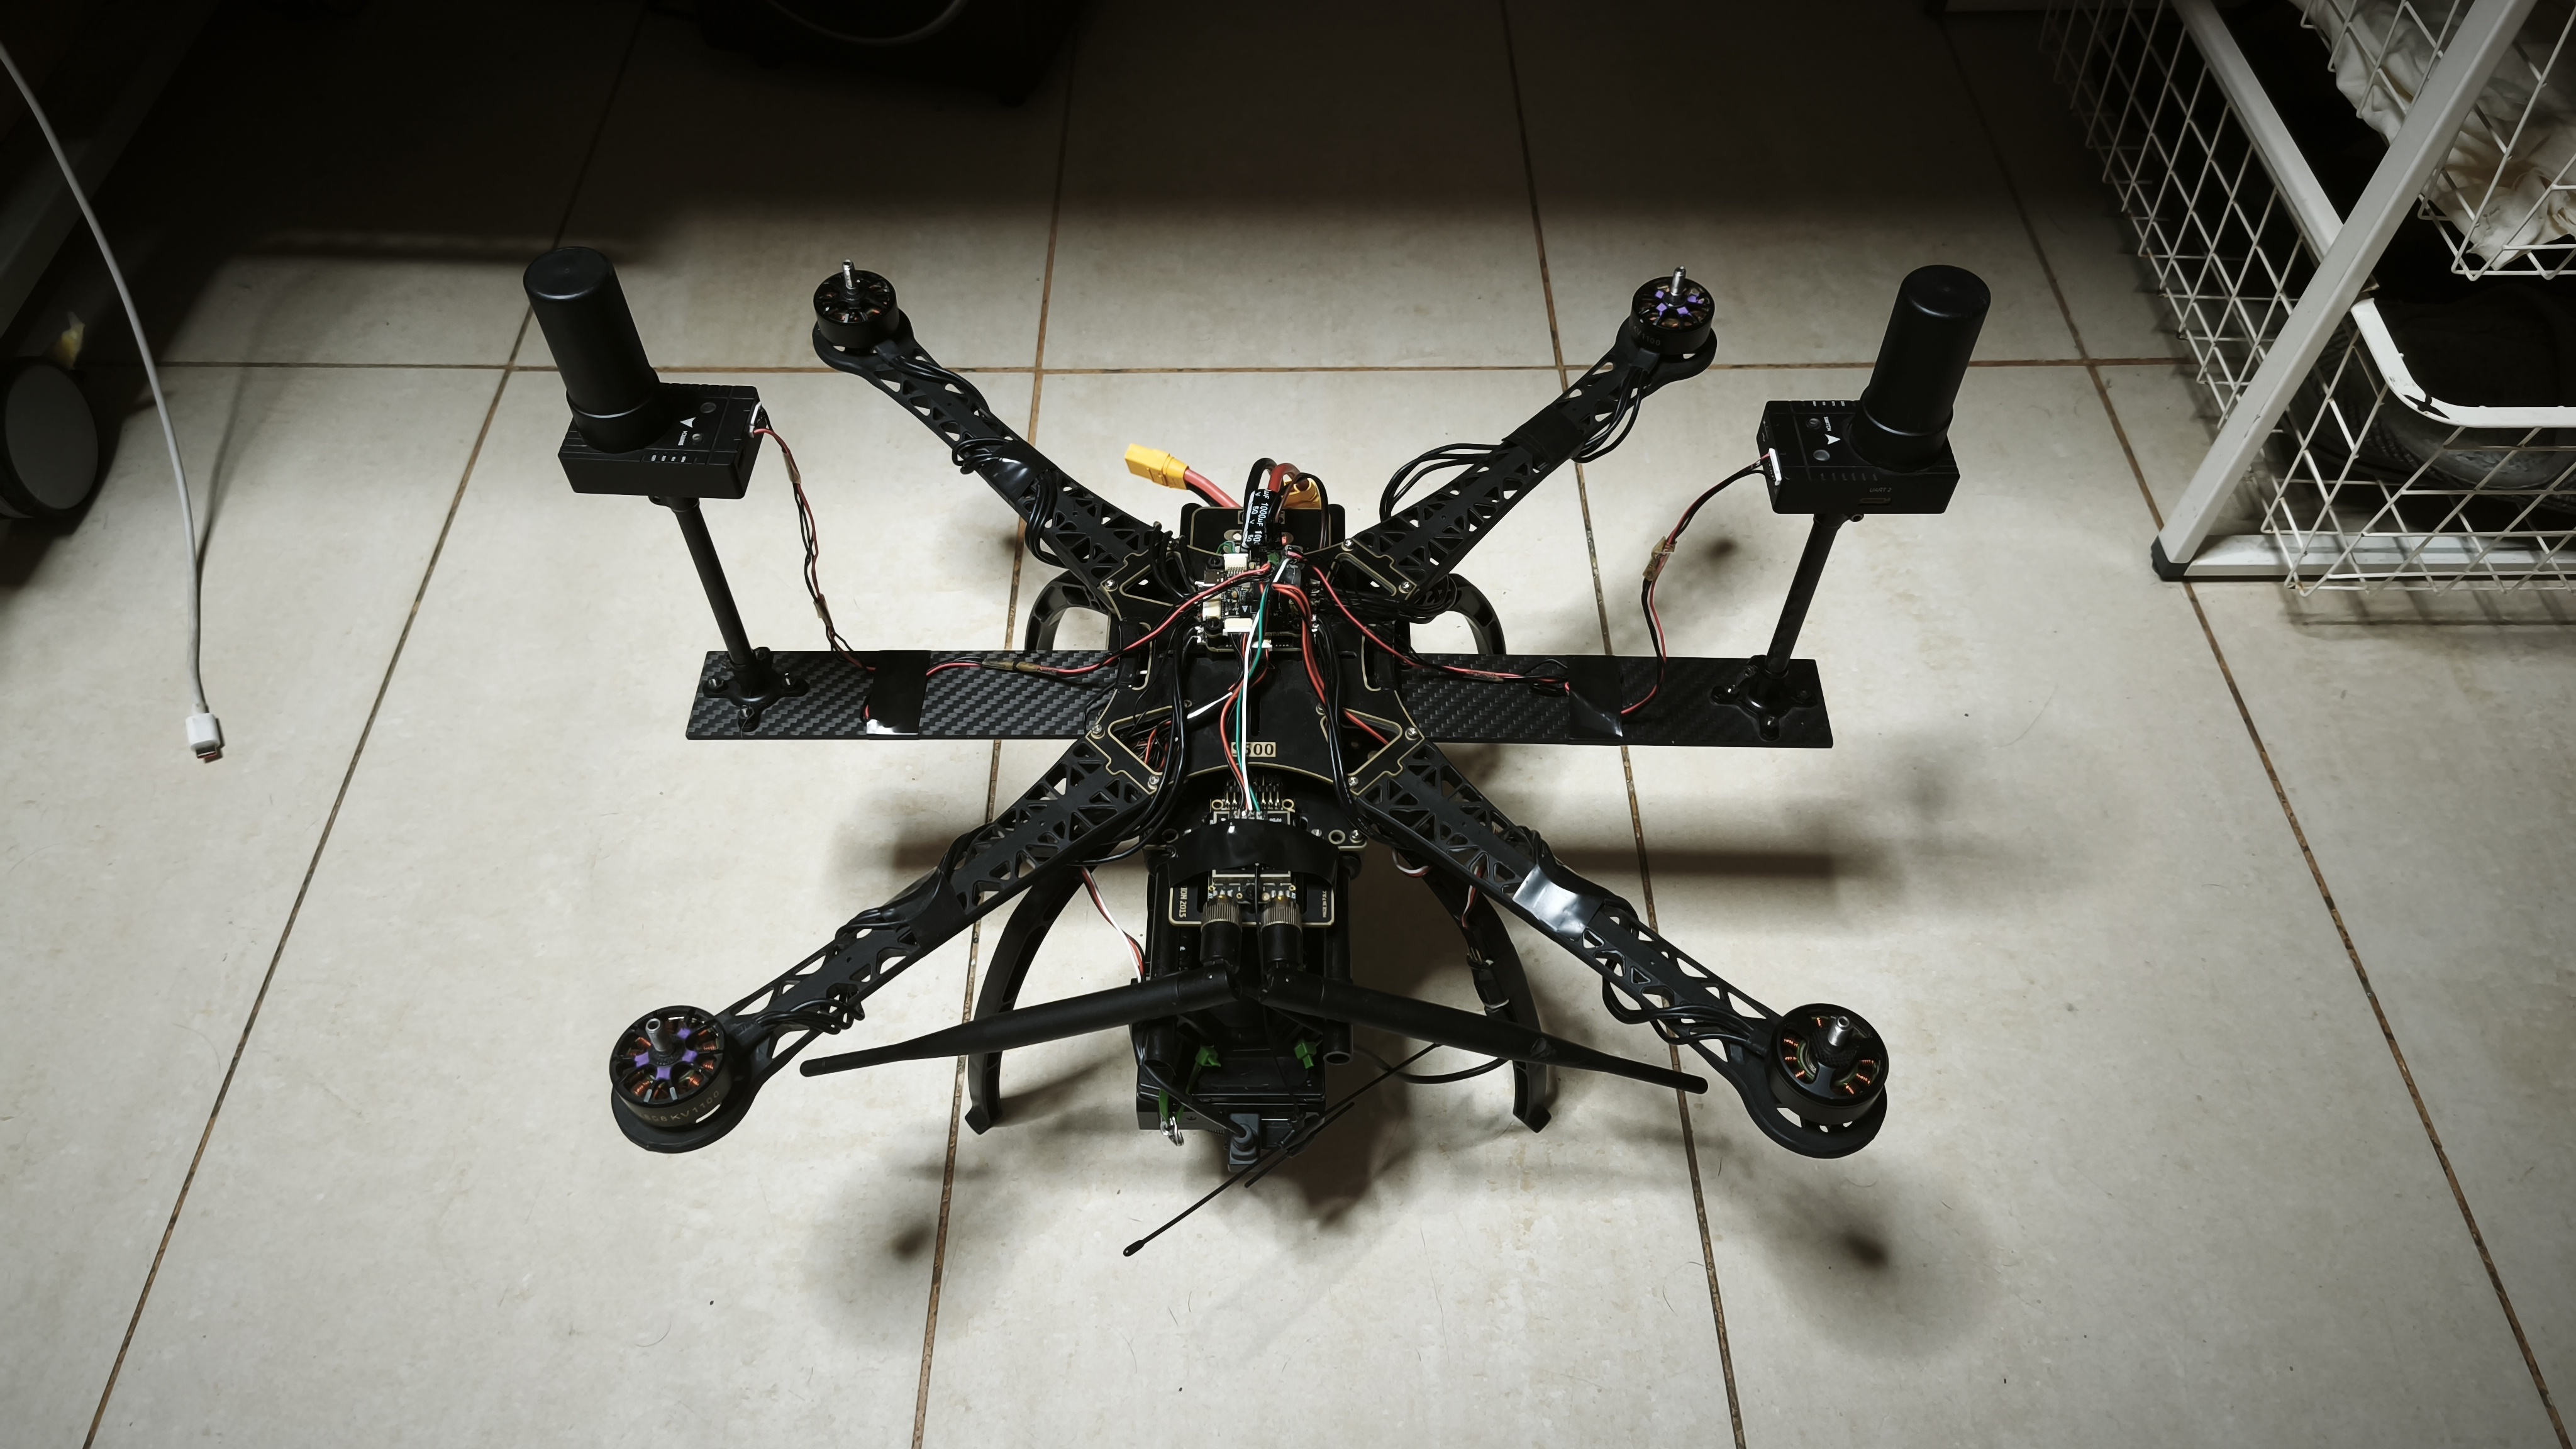
\includegraphics[width=0.75\textwidth]{img/xasis_sencer.jpg}
\end{titlepage}

\chapter*{Summary}
\addcontentsline{toc}{chapter}{Summary}

This document describes the design, construction and commissioning of a precision aerial photogrammetry system made of three subsystems: an RTK GNSS base of its own, a UAV with two GNSS receivers in \emph{moving baseline} and a camera with hot-shoe timing, and a ground station that links them. The goal is the centimetre-level geotagging of aerial photographs to produce orthomosaics and digital surface models, with a hardware cost of about €2,150 and full control over the firmware, the corrections and the data flow.

The main results are:
\begin{itemize}
    \item An architecture that serves RTCM3 corrections over local WiFi and forwards them to the drone over a long-range telemetry link, and that obtains RTK Fixed for 100~\% of the flight on both receivers, with GNSS-derived yaw and no magnetic compass.
    \item A flight-test campaign that, from log analysis, resolved control oscillations, a moving-baseline configuration failure, the collapse of a battery and the camera triggering problems (\cref{chap:proves-vol}).
    \item Two photogrammetry flights processed end to end: 118 photographs reconstructed at 30~m, with a GSD of 0.45~cm/px and a reprojection error of 0.90~px, and 110 at 50~m (\cref{chap:vols-prova}).
    \item The measurement, by two independent methods, of an effective shutter delay of 0.27--0.28~s ($\sim$1.3~m at 5~m/s), which justifies the hot-shoe feedback and is compensated in the geotagging.
    \item An analysis of the propulsion group that identifies the propeller diameter as the limiting factor for endurance and quantifies the room for improvement (\cref{sec:propulsor}).
\end{itemize}

The accuracy of the final product cannot yet be stated: it requires ground control and check points measured with the same base as the flight, planned in the precision test plan (\cref{sec:validacio}). Because the base runs a \emph{survey-in} in every session, the absolute position of the map has an offset of the order of metres that can only be corrected with the base log. The document marks with a \emph{Pending} box the documentation and tests that are still missing, and the consolidated task list is in \cref{sec:pendents-proves-vol}.

\tableofcontents

\mainmatter

% =====================================================
% PART I — DESIGN AND CONSTRUCTION
% =====================================================
\part{Design and construction}
\chapter{System design and construction}
\label{chap:construccio}

\section{Introduction}
\label{sec:introduccio}

This document describes the design, construction and in-flight validation of a complete precision aerial photogrammetry system (drone \emph{surveying}): an RTK GNSS base of its own, a UAV with two GNSS receivers and a camera with hot-shoe timing, and a ground station that links them.

The goal is centimetre-level geotagging of aerial photographs ($\leq 2$~cm horizontal, $\leq 3$~cm vertical) to produce survey-grade orthomosaics and digital surface models, with a total hardware cost of around €2,150 --~a fraction of the cost of a DJI P4 RTK or of an Emlid~+~UAV set~-- and with full control over the \emph{firmware}, the corrections and the data flow.

The system is divided into three subsystems:
\begin{itemize}
    \item \textbf{RTK GNSS base}: fixed station that generates RTCM3 corrections.
    \item \textbf{UAV (\emph{rover})}: drone with two GNSS receivers for RTK positioning and \emph{moving baseline} heading.
    \item \textbf{Ground station (GS)}: telemetry link and relay of the corrections to the drone.
\end{itemize}

The document is organised in four blocks: design and construction (this chapter), the operation manual and procedures (\cref{chap:manual}), the flight-test and tuning campaign (\cref{chap:proves-vol}) and the photogrammetry flights that result from it (\cref{chap:vols-prova}).

\section{Architecture and data flow}
\label{sec:arquitectura}

The chosen architecture uses the base to serve RTCM3 corrections over local WiFi (\emph{access point} mode) through a TCP server of its own, without NTRIP. A direct base~$\rightarrow$~drone radio link was discarded to simplify the system (a single radio channel to the drone) and to gain resilience in rural areas without mobile coverage.

\begin{figure}[H]
    \centering
    \resizebox{\linewidth}{!}{%
    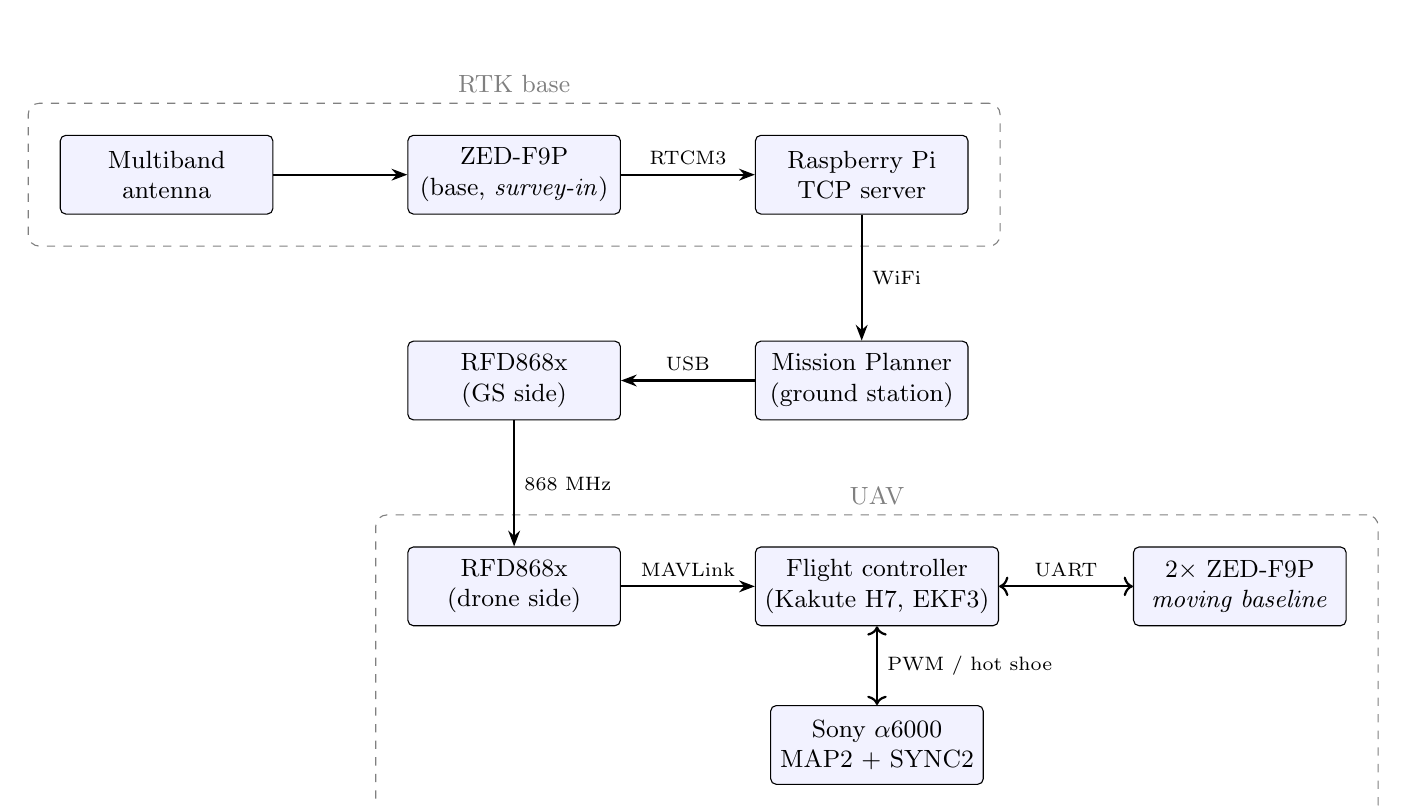
\begin{tikzpicture}[
        box/.style={draw, rounded corners=2pt, align=center, font=\small, minimum height=10mm, minimum width=27mm, fill=blue!5},
        arr/.style={-{Stealth[length=2mm]}, thick},
        grp/.style={draw, dashed, rounded corners=4pt, inner sep=4mm, gray},
        node distance=8mm and 17mm]
        \node[box] (ant) {Multiband\\antenna};
        \node[box, right=of ant] (f9b) {ZED-F9P\\(base, \emph{survey-in})};
        \node[box, right=of f9b] (pi) {Raspberry Pi\\TCP server};
        \node[box, below=16mm of pi] (gs) {Mission Planner\\(ground station)};
        \node[box, left=of gs] (rfdg) {RFD868x\\(GS side)};
        \node[box, below=16mm of rfdg] (rfdu) {RFD868x\\(drone side)};
        \node[box, right=of rfdu] (fc) {Flight controller\\(Kakute H7, EKF3)};
        \node[box, right=of fc] (gnss) {2$\times$ ZED-F9P\\\emph{moving baseline}};
        \node[box, below=10mm of fc] (cam) {Sony $\alpha$6000\\MAP2 + SYNC2};
        \draw[arr] (ant) -- (f9b);
        \draw[arr] (f9b) -- node[above, font=\scriptsize] {RTCM3} (pi);
        \draw[arr] (pi) -- node[right, font=\scriptsize] {WiFi} (gs);
        \draw[arr] (gs) -- node[above, font=\scriptsize] {USB} (rfdg);
        \draw[arr] (rfdg) -- node[right, font=\scriptsize] {868~MHz} (rfdu);
        \draw[arr] (rfdu) -- node[above, font=\scriptsize] {MAVLink} (fc);
        \draw[arr, <->] (fc) -- node[above, font=\scriptsize] {UART} (gnss);
        \draw[arr, <->] (fc) -- node[right, font=\scriptsize] {PWM / hot shoe} (cam);
        \begin{scope}[on background layer]
            \node[grp, fit=(ant)(f9b)(pi), label={[font=\small, gray]above:RTK base}] {};
            \node[grp, fit=(rfdu)(fc)(gnss)(cam), label={[font=\small, gray]above:UAV}] {};
        \end{scope}
    \end{tikzpicture}}
    \caption{Block diagram of the system and flow of the RTCM3 corrections.}
    \label{fig:diagrama-blocs}
\end{figure}

\subsection{Complete data flow}

\begin{enumerate}[label=\arabic*.]
    \item The multiband antenna receives L1/L2/L5 (GPS, GLONASS, Galileo, BeiDou).
    \item The base \textbf{ZED-F9P} (\emph{survey-in} mode in every session, \cref{sec:protocol-camp}) generates \textbf{RTCM3} messages (1005, 1074, 1084, 1094, 1124 and 1230) at 1~Hz. Message 1005, with the base position, is only emitted when the \emph{survey-in} is valid.
    \item The \textbf{Raspberry Pi} receives these messages over USB (serial port of the simpleRTK2B Pro receiver) and redistributes them as they arrive through the TCP server on port 5000, over WiFi AP.
    \item The \textbf{GS} (Mission Planner / QGroundControl at the pilot's side) connects to the TCP server and forwards the RTCM3 stream to the drone over MAVLink (\texttt{GPS\_RTCM\_DATA}) through the \textbf{RFD868x} pair.
    \item On the drone, the primary F9P receives the corrections, computes the RTK position and, in \emph{moving baseline} mode, generates RTCM 4072.x for the secondary to derive the \emph{heading}.
    \item The \textbf{FC} integrates the RTK position and the GNSS \emph{yaw} in the EKF3 for navigation and geotagging.
\end{enumerate}

\section{Design decisions}
\label{sec:decisions}

\begin{description}
    \item[Moving baseline with 2$\times$ ZED-F9P] instead of a UM982 with native \emph{heading}. The F9P is better documented, has more community support and is interchangeable between base and UAV. It provides GPS-for-yaw, which makes it possible to do without the magnetic compass --~an important advantage on \emph{frames} with a lot of current.
    \item[RFD868x for the GS$\leftrightarrow$UAV link] at 868~MHz (European band) it allows up to 500~mW EIRP and a range above 40~km. Always the European 868 version (never 915 or 433).
    \item[Local TCP server over WiFi] robust in the absence of mobile coverage; in practice it is almost always operated locally (park the vehicle, set up the tripod next to it and fly).
    \item[Hot-shoe feedback (Seagull SYNC2)] solves the variable shutter latency ($\sim$100~ms equals 1.5~m of error at 15~m/s). Without this \emph{feedback} there is no real centimetre-level precision in the geotagging; \cref{sec:retard-obturador} quantifies the effect.
    \item[Optional PPK post-processing] logging of raw \texttt{UBX} data at the base and on the drone, which gives a solution independent of the quality of the real-time RTK link.
\end{description}

\section{Bill of materials}
\label{sec:materials}

The hardware of the system has a total cost of €2,150.

\subsection{Drone}

\begin{table}[H]
    \centering
    \caption{Drone components (UAV/\emph{rover})}
    \label{tab:materials-dron}
    \begin{tabular}{lll}
        \toprule
        Component & Model & Approx. cost \\
        \midrule
        \emph{Frame} & S500 (Quad X, 500~mm between axes) & €35 \\
        Motors (4$\times$) & Pilotix 2808, 1100~KV & €60 \\
        ESC & Hobbywing XRotor 65A 4-in-1 (DShot) & €30 \\
        FC & Holybro Kakute H7 (STM32H7) & €55 \\
        GPS (2$\times$) & Holybro H-RTK F9P Helical & €510 (€255 each) \\
        Telemetry & RFD868x EU 500~mW (drone + GS pair) & €363 \\
        RC & Radiomaster XR1 Nano ELRS dual-band & €16 \\
        Battery & Gaoneng GNB 6S 4000~mAh 70C & €70 \\
        \bottomrule
    \end{tabular}
\end{table}

\begin{description}
    \item[Pilotix 2808 motors, 1100~KV] moderate KV for 6S, intended for 8-inch propellers (\cref{tab:kv-compatibilitat}) with the additional payload of the RTK~+~camera system, instead of the high KV typical of \emph{freestyle}, which sacrifice efficiency for speed. The 7-inch propellers of the initial build were used for availability, not by design (\cref{subsec:propulsor-inicial}).
    \item[Hobbywing XRotor 65A 4-in-1 ESC (DShot)] current margin for the additional weight; bidirectional DShot gives per-motor RPM telemetry, useful for vibration diagnosis; the 4-in-1 format simplifies the power wiring.
    \item[Holybro Kakute H7 FC (STM32H7)] enough UART ports for the whole architecture without any expansion (2$\times$F9P, RFD868x, ELRS RC, ESC telemetry, USB) and native ArduPilot support for \emph{moving baseline} GPS and DShot.
    \item[Holybro H-RTK F9P Helical GPS (2$\times$)] integrated module (helical antenna + F9P \emph{breakout}) already designed for \emph{moving baseline} with ArduPilot; avoids having to design and match antenna and \emph{breakout} separately.
    \item[RFD868x telemetry] full justification in \cref{sec:decisions}.
    \item[Radiomaster XR1 Nano ELRS RC] minimum size and weight so as not to penalise the payload; low-latency ELRS complements the RFD868x, which carries the MAVLink/RTCM data but not the flight control.
    \item[Gaoneng 6S 4000~mAh 70C battery] 6S for better voltage efficiency with the additional consumption (GPS, telemetry, camera); 70C gives enough peak-current margin with the 4 motors at full load.
\end{description}

\subsection{GNSS base}

\begin{table}[H]
    \centering
    \caption{RTK base components}
    \label{tab:materials-base}
    \begin{tabular}{lll}
        \toprule
        Component & Model & Approx. cost \\
        \midrule
        GNSS & ArduSimple simpleRTK2B Pro (ZED-F9P) & €126 \\
        Antenna & BD900 GNSS (multiband) & €43 \\
        SBC & Raspberry Pi Zero W & €35 \\
        Power & Waveshare UPS HAT + 2$\times$ 18650 3500~mAh & €47 \\
        \bottomrule
    \end{tabular}
\end{table}

\begin{description}
    \item[simpleRTK2B Pro GNSS (ZED-F9P)] development board with USB and an SMA antenna connector, with the same chip as the drone receivers, which gives interchangeability and a shared configuration and \emph{firmware} (\cref{sec:decisions}).
    \item[BD900 GNSS antenna (multiband)] necessary to receive the two bands and the multiple constellations used by the ZED-F9P, a requirement for the \emph{survey-in} to converge (\cref{sec:protocol-camp}).
    \item[Raspberry Pi Zero W] small size and low consumption for field use on battery, with enough capacity to distribute the corrections through the TCP server and act as a WiFi access point (NetworkManager).
    \item[UPS HAT + 2$\times$18650 power] base endurance independent of the mains in the field, with protection against cuts during logging.
\end{description}

\subsection{Ground station}

\begin{table}[H]
    \centering
    \caption{Ground station (GS) components}
    \label{tab:materials-gs}
    \begin{tabular}{lll}
        \toprule
        Component & Model & Approx. cost \\
        \midrule
        Transmitter & Radiomaster TX16S (or similar) ELRS & €167 \\
        Telemetry & RFD868x (GS side, included in the pair) & -- \\
        Laptop / tablet & Own, with Mission Planner & -- \\
        \bottomrule
    \end{tabular}
\end{table}

The transmitter and the RFD868x pair are standard items with no specific design decision. The only additional element of the GS is the laptop or tablet with Mission Planner or QGroundControl, which bridges the base TCP server and the MAVLink stream to the drone (\cref{sec:arquitectura}).

\subsection{Camera (mapping module)}

\begin{table}[H]
    \centering
    \caption{Camera module for photogrammetry}
    \label{tab:materials-camera}
    \begin{tabular}{lll}
        \toprule
        Component & Model & Approx. cost \\
        \midrule
        Body & Sony $\alpha$6000 (24~MP APS-C, second hand) & €200 \\
        Lens & TTArtisan 25~mm f/2 APS-C, manual focus & €71 \\
        \emph{Trigger} & Seagull MAP2 (fires by PWM) & €30 \\
        \emph{Feedback} & Seagull SYNC2 (hot shoe, X-sync $\rightarrow$ FC) & €30 \\
        SD card & 3$\times$ SanDisk Extreme 64~GB & €45 \\
        \bottomrule
    \end{tabular}
\end{table}

\begin{description}
    \item[Sony $\alpha$6000 body] large APS-C sensor (good signal-to-noise ratio) with 24~MP resolution, in a reasonable body size and weight for the drone; second hand to keep the cost down.
    \item[TTArtisan 25~mm f/2] short focal length for a wide field of view (more coverage per flight pass and fewer passes needed) and enough speed for short exposures. Manual focus allows fixing the focus at infinity and prevents the autofocus from hunting during flight, which matters for photogrammetry. Compact, light metal construction, at a much lower cost than a native lens.
    \item[\emph{Trigger} Seagull MAP2] remote PWM trigger from the FC without having to modify the camera electronically.
    \item[\emph{Feedback} Seagull SYNC2] mandatory for centimetre-level geotagging precision; justification in \cref{sec:decisions}.
\end{description}

\subsection{Extras and consumables}

JST-GH cables, XT60/XT90 connectors, M3 \emph{standoffs}, carbon \emph{bracket} for the helical antennas, 5/8-inch-thread survey tripod, LMR-240 coaxial cable, TNC/SMA connectors with IP54 protection, microSD cards and tools (soldering iron, JST-GH crimper, multimeter), at a total cost of about €218.

\section{Assembly}
\label{sec:muntatge}

\subsection{Drone (UAV)}
\label{subsec:muntatge-dron}

The drone is built on an S500 \emph{frame} in X configuration, 500~mm between axes. A side carbon plate is mounted on the central board and acts as the \emph{baseline} \emph{bracket}: at each end there is a vertical carbon post carrying a Holybro H-RTK F9P Helical module, so that the two antennas are parallel, pointing up, at the highest point of the aircraft (\cref{fig:xassis-base}). The separation between antennas is 0.38~m along the lateral axis of the drone (\cref{sec:antenes-gnss}). The RFD868x telemetry module, with its two antennas, is fixed on the top plate and connected to the flight controller by UART.

\begin{figure}[H]
    \centering
    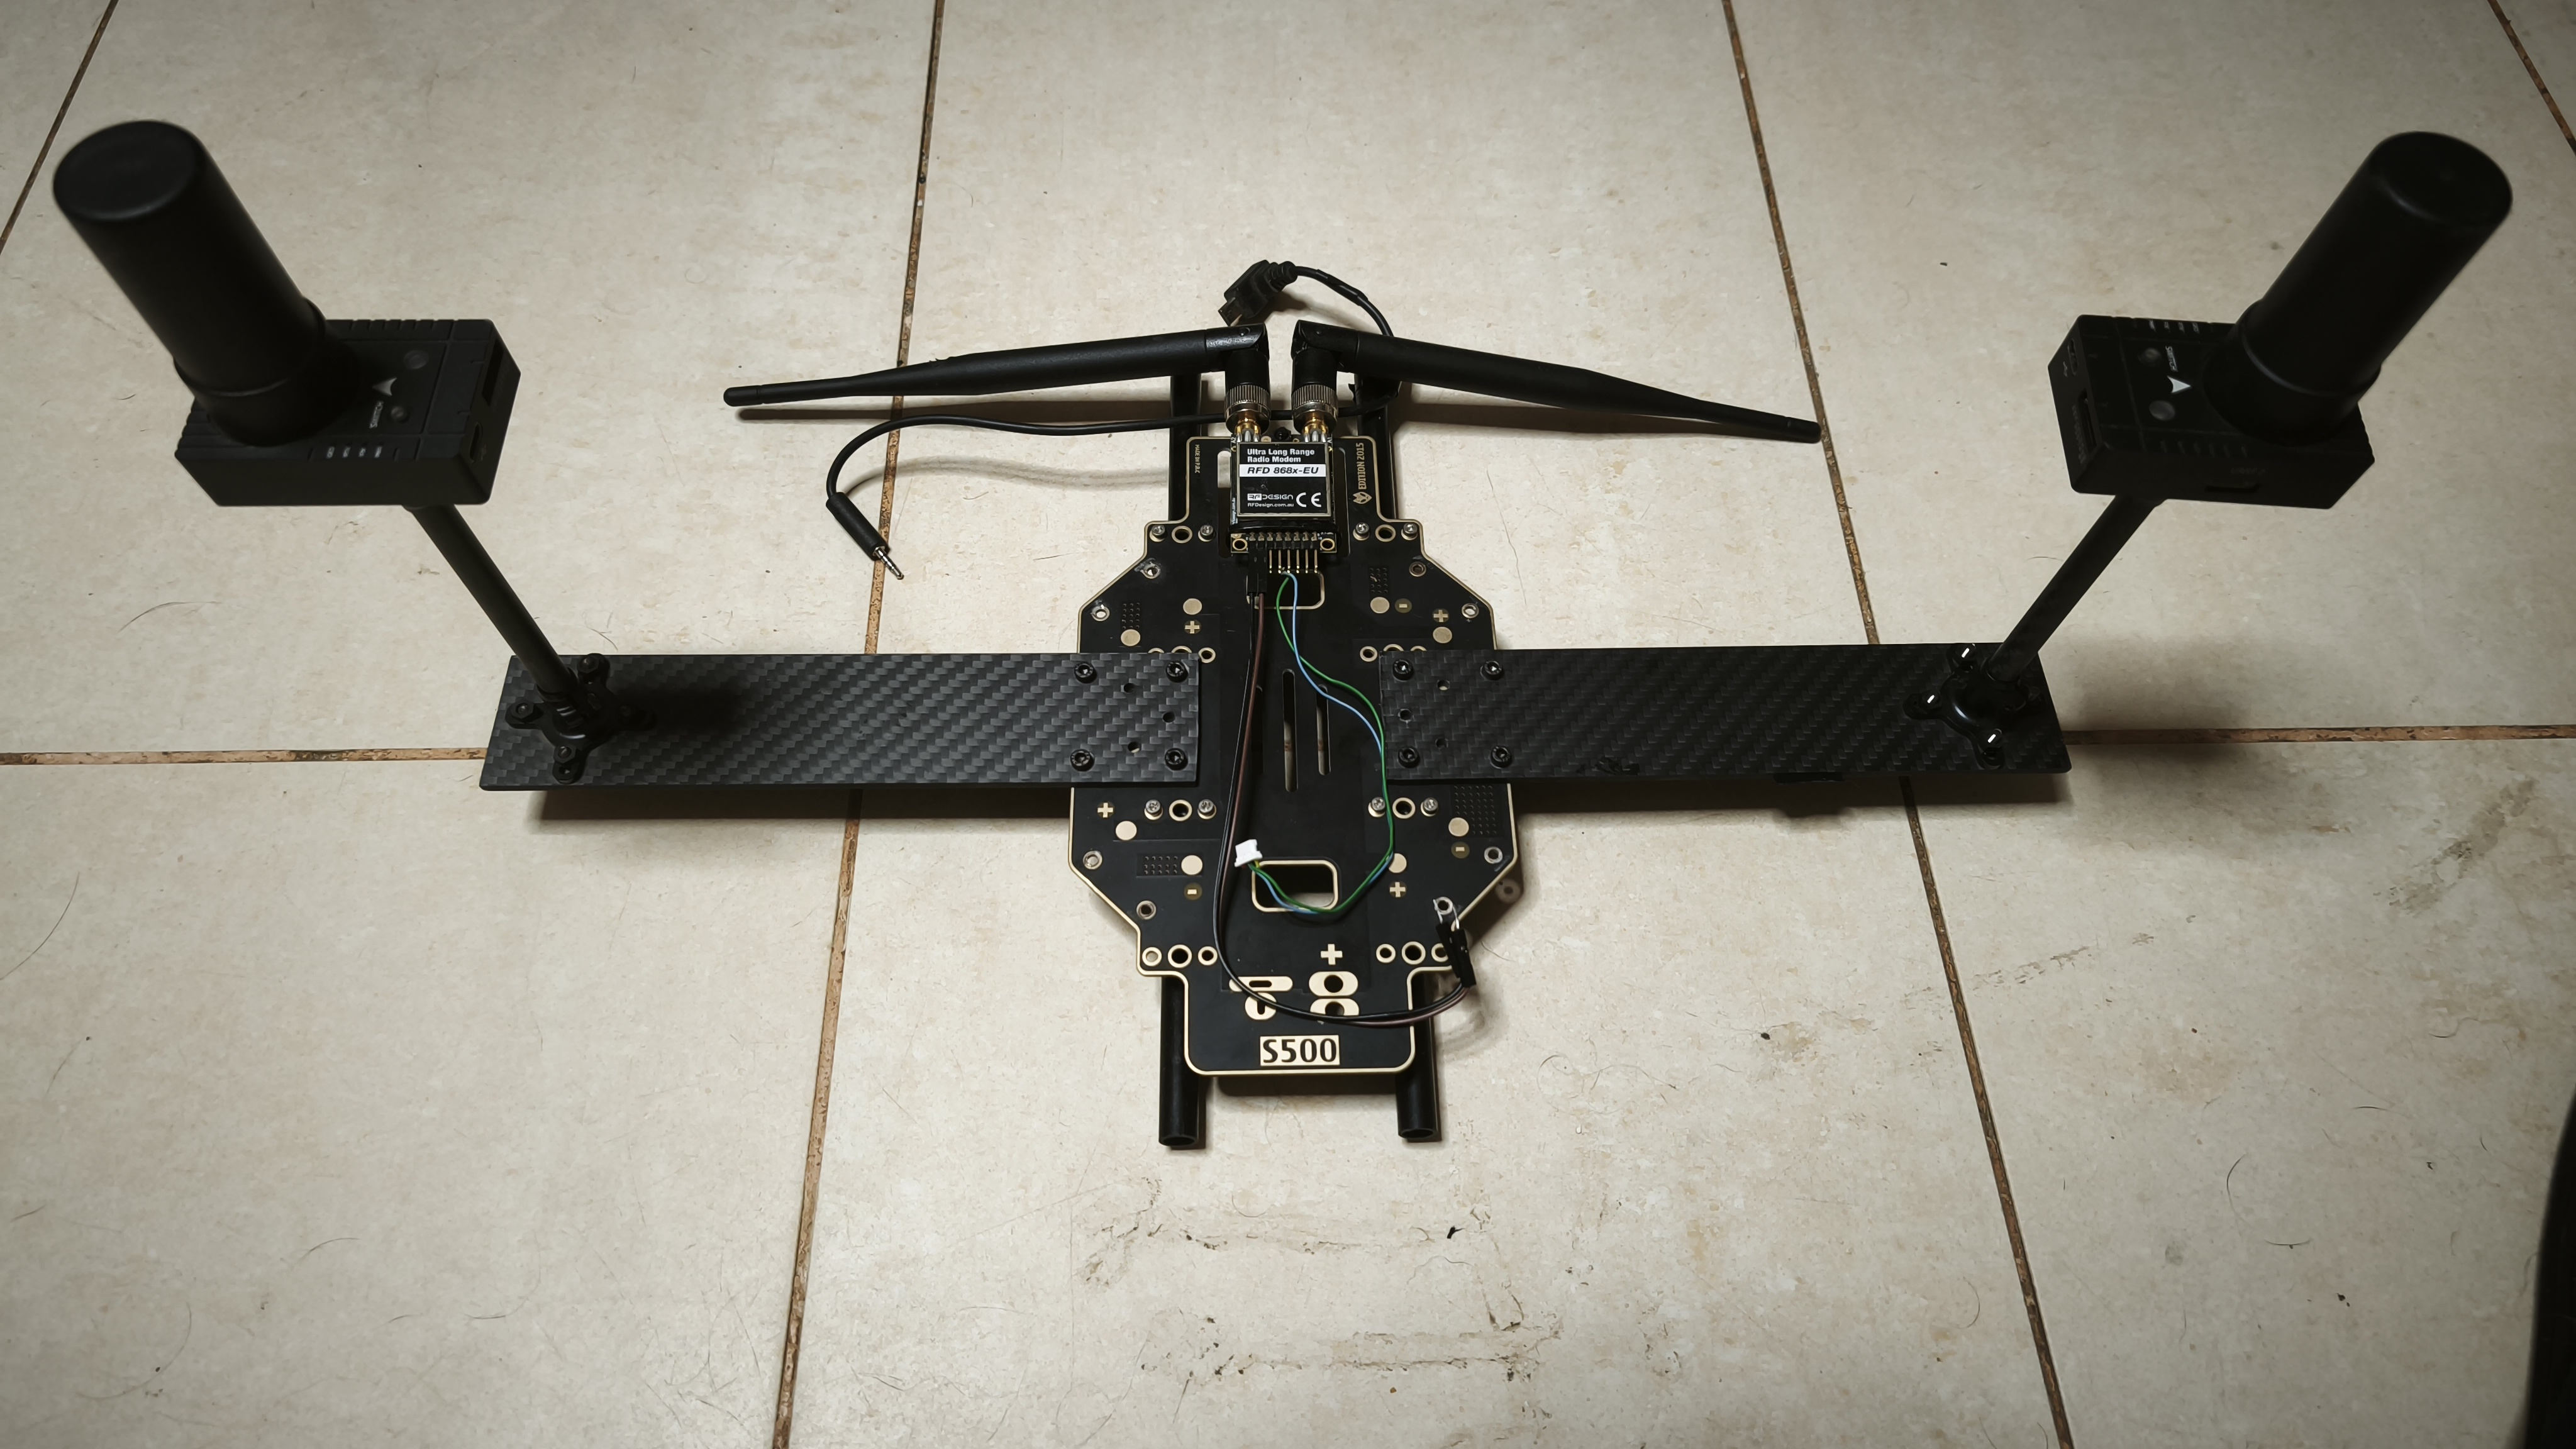
\includegraphics[width=\textwidth]{img/xasis_base.jpg}
    \caption{S500 central board with the carbon \emph{bracket}, the two H-RTK F9P Helical modules on vertical posts and the RFD868x module.}
    \label{fig:xassis-base}
\end{figure}

\begin{figure}[H]
    \centering
    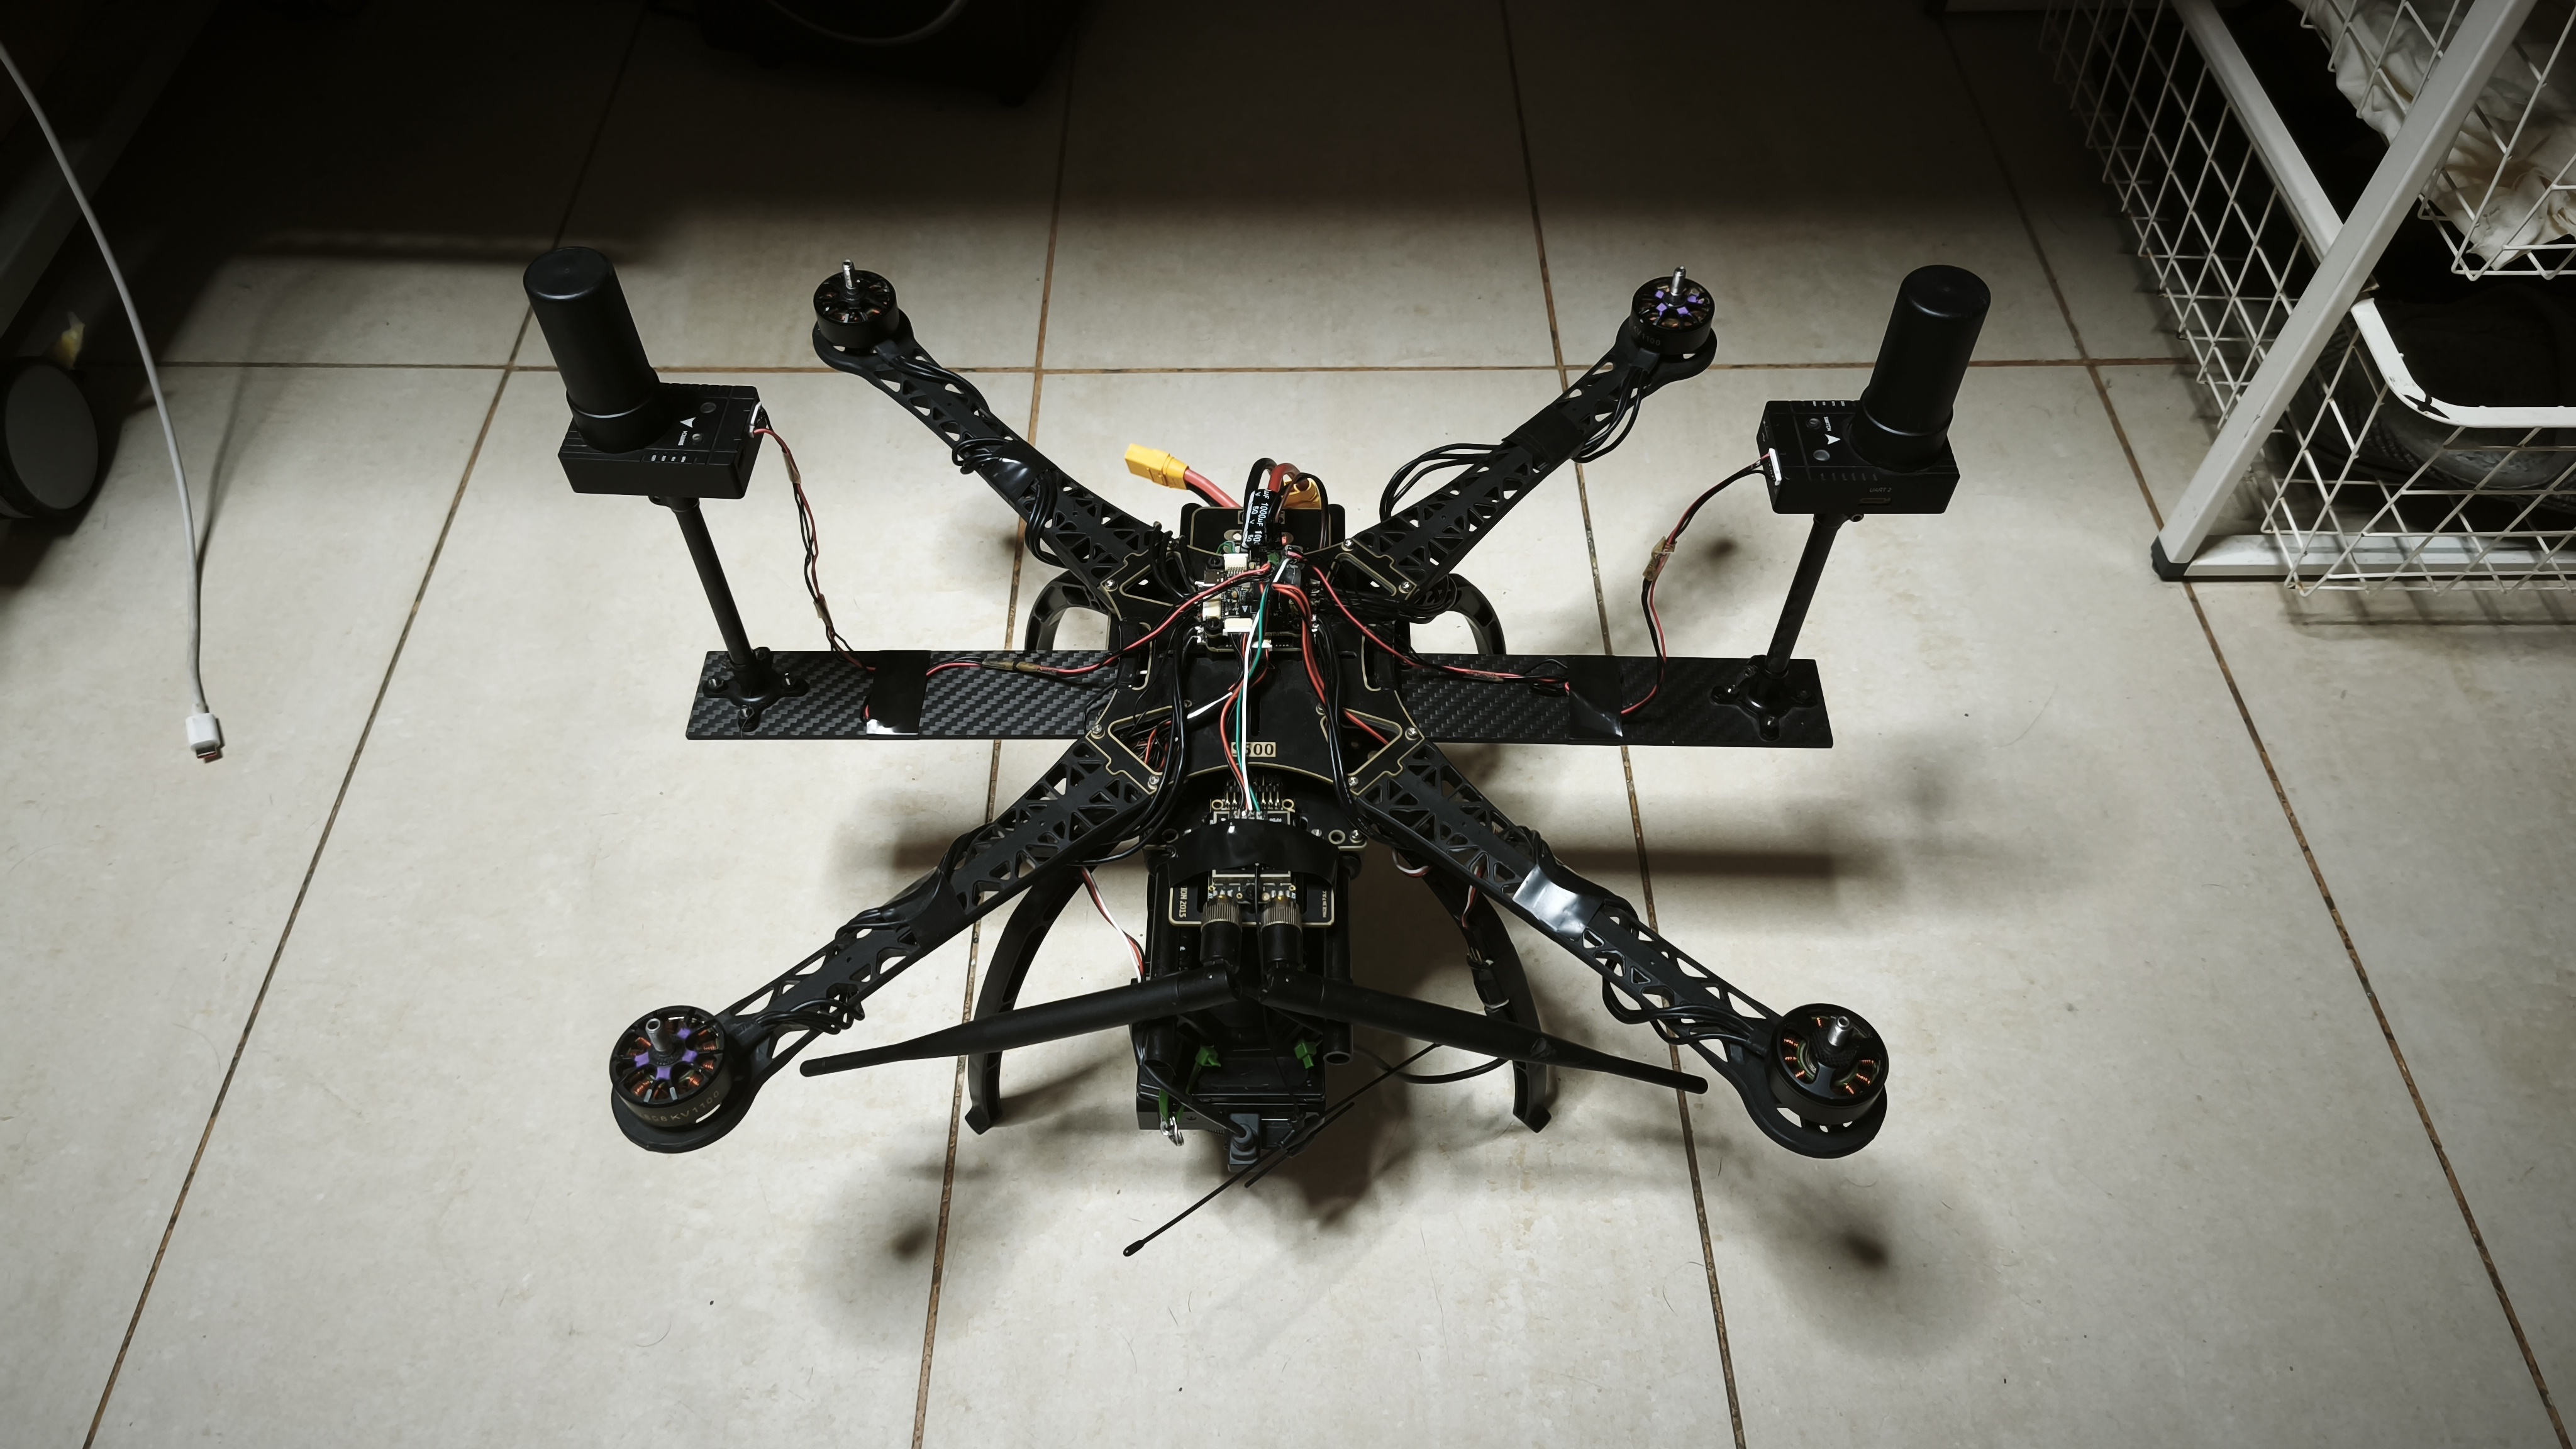
\includegraphics[width=\textwidth]{img/xasis_sencer.jpg}
    \caption{Finished drone seen from above: motors, lateral \emph{baseline} with the two GNSS antennas, telemetry module and landing gear.}
    \label{fig:xassis-sencer}
\end{figure}

Under the \emph{frame} there is a rail made of two parallel carbon bars with clamps (\cref{fig:xassis-abaix}), which supports both the camera and the battery. The camera (Sony $\alpha$6000 with the 25~mm lens) points at nadir, with the Seagull SYNC2 on the hot shoe; the 6S battery is fixed to the same rail, so that the centre of gravity is close to the vertical axis of the drone.

\begin{figure}[H]
    \centering
    \begin{subfigure}[b]{0.49\textwidth}
        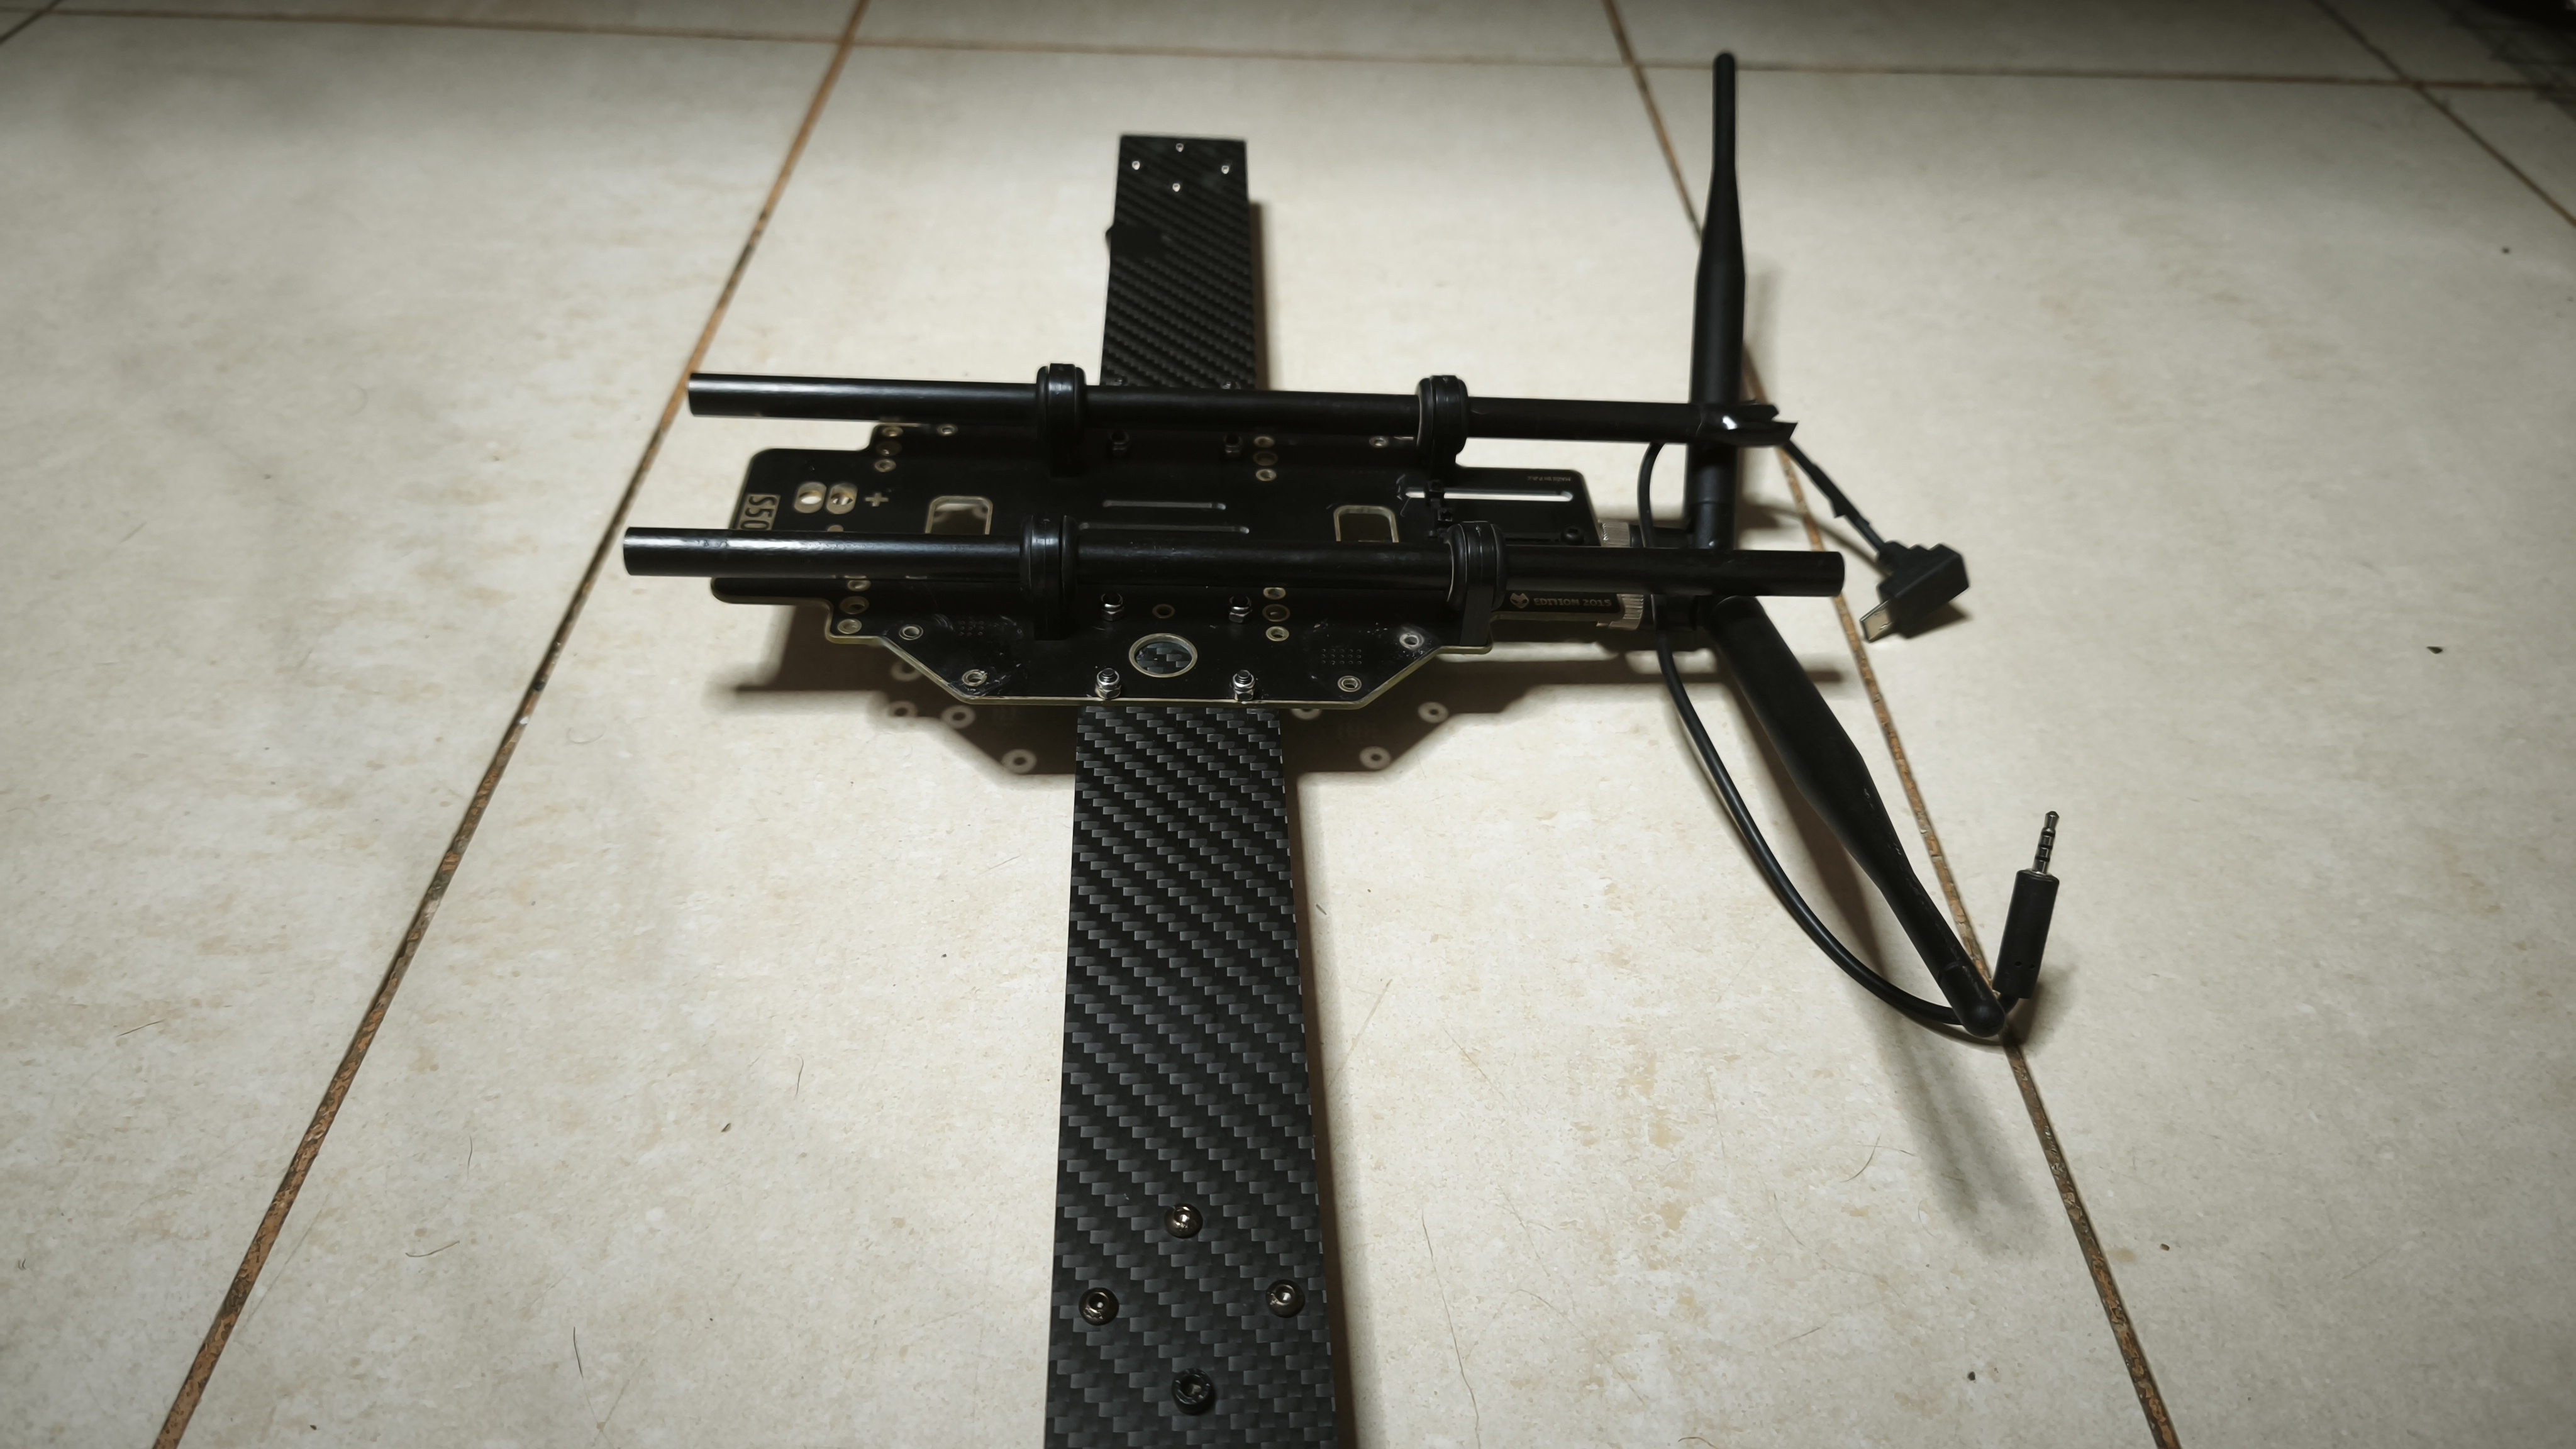
\includegraphics[width=\textwidth]{img/xasis_abaix_buit.jpg}
        \caption{Lower rail without load.}
    \end{subfigure}
    \hfill
    \begin{subfigure}[b]{0.49\textwidth}
        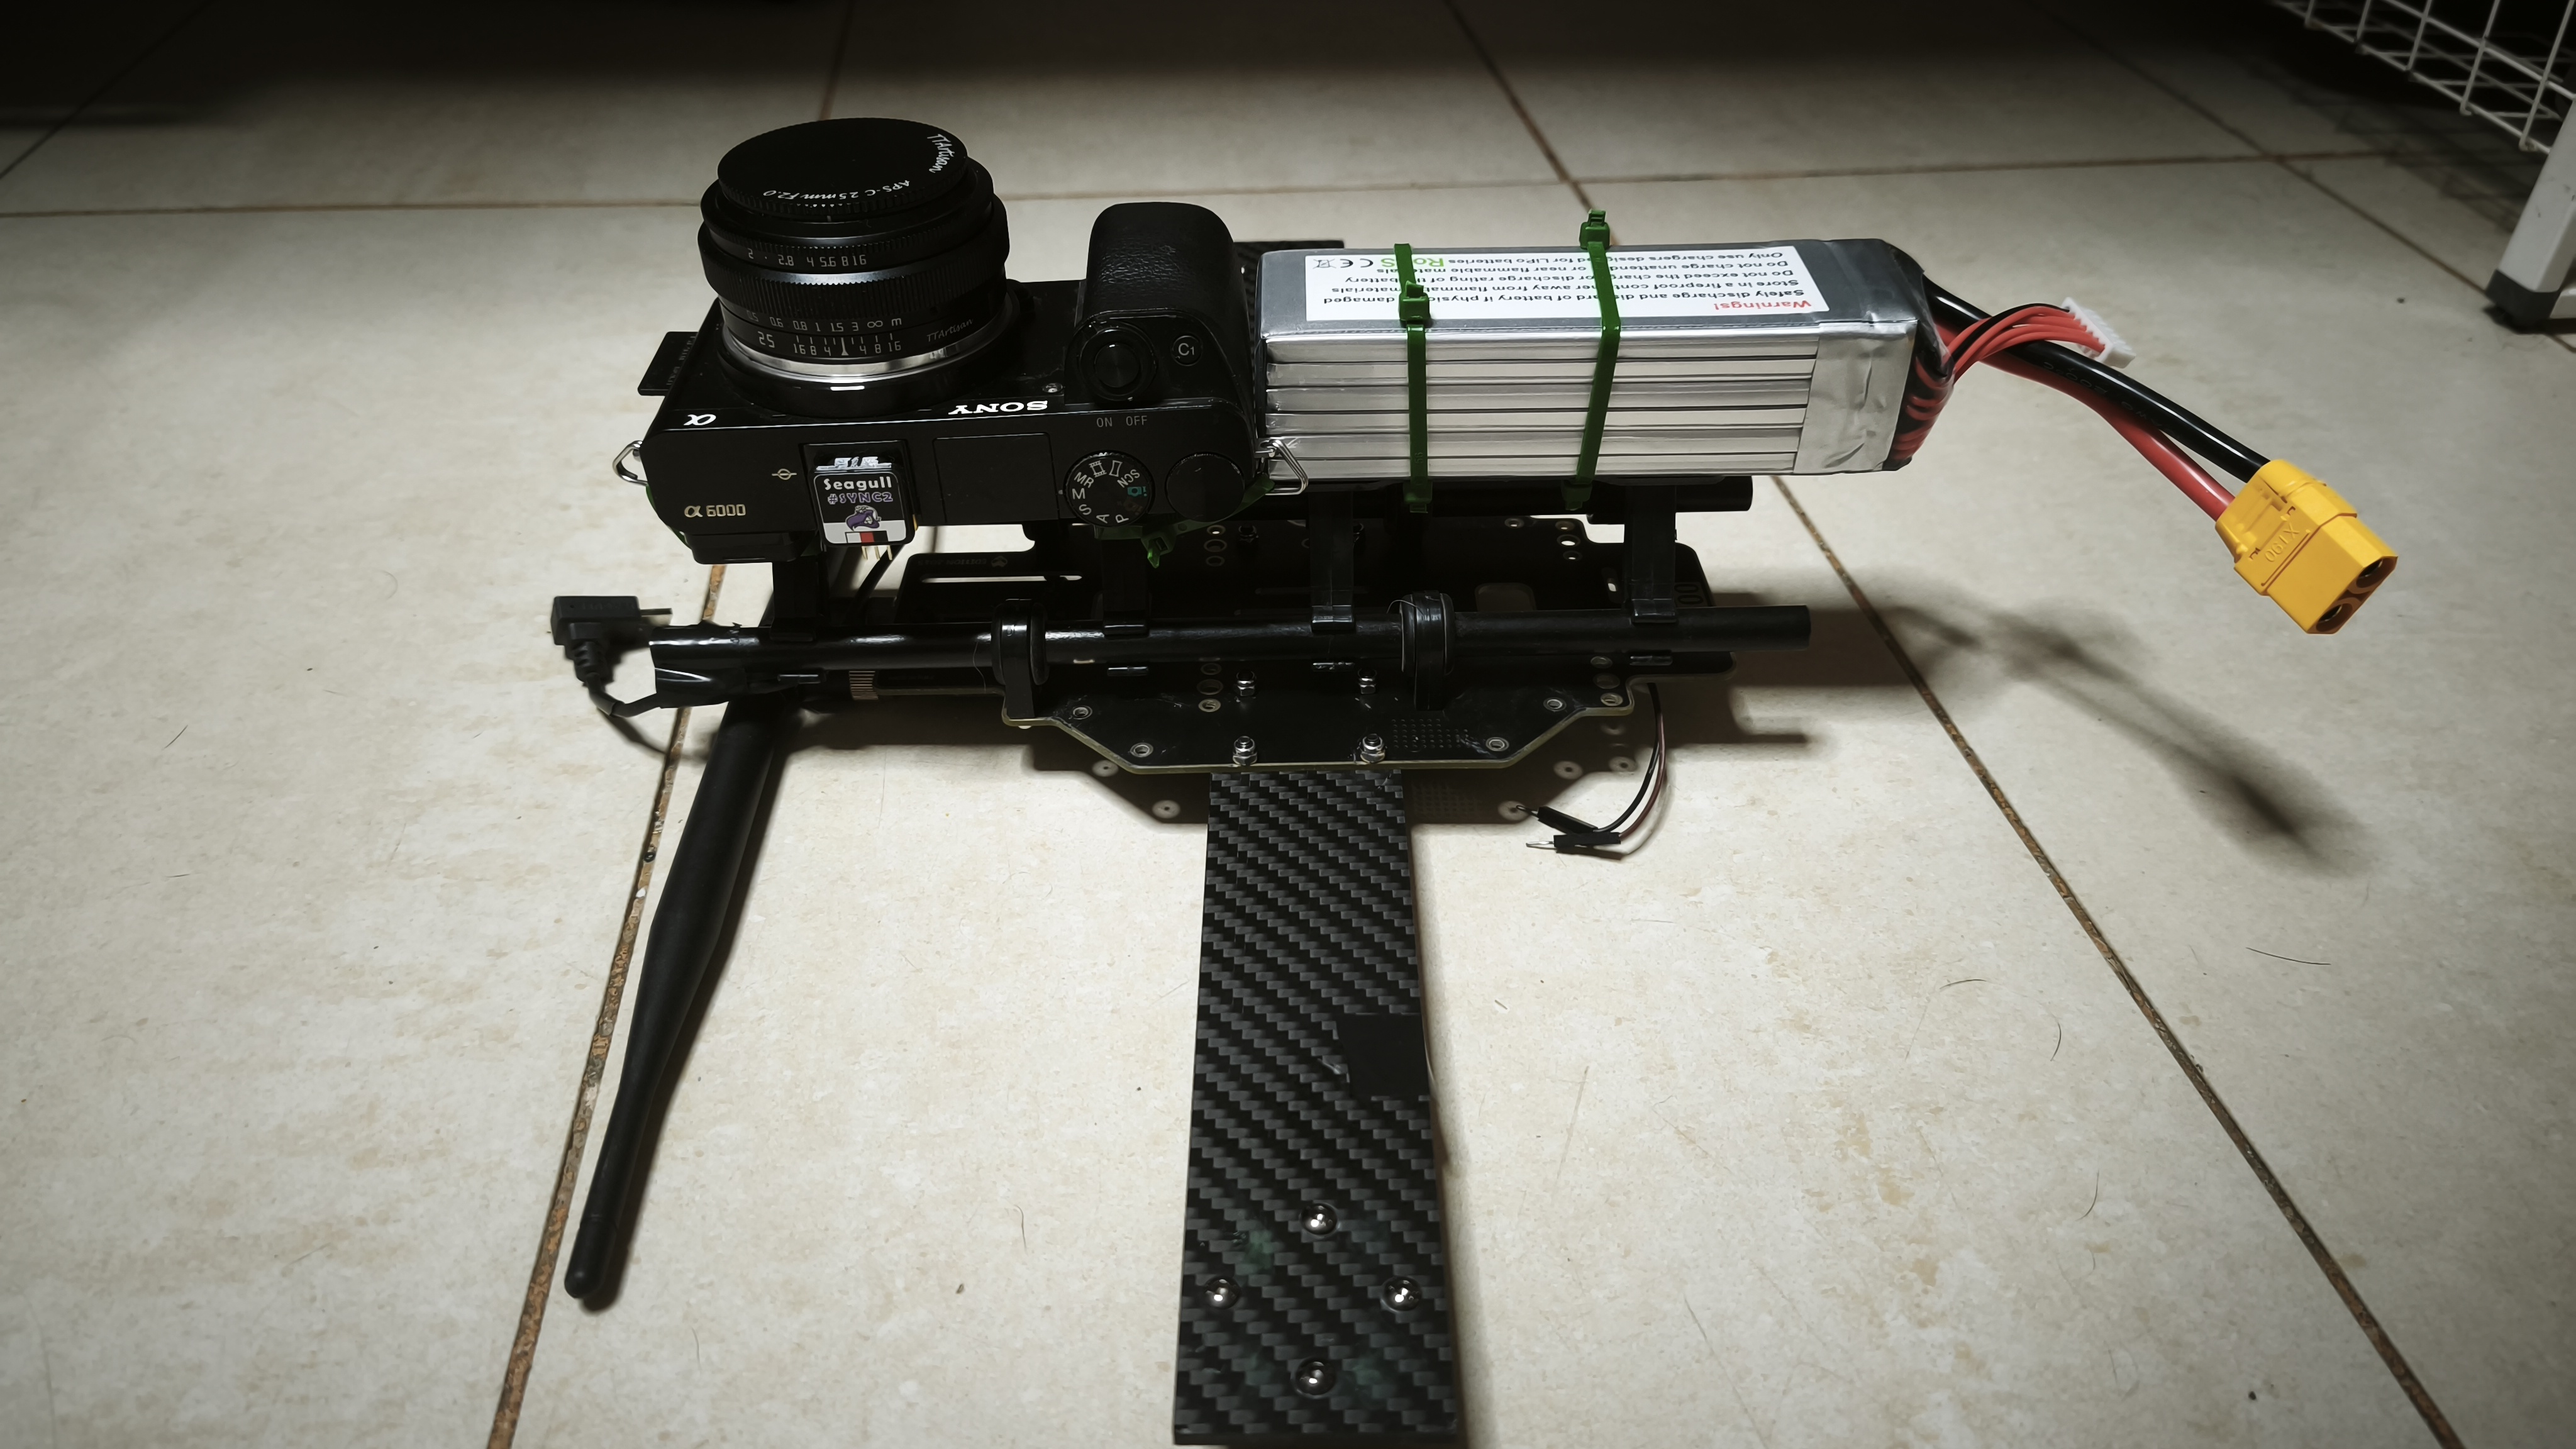
\includegraphics[width=\textwidth]{img/xasis_abaix_ple.jpg}
        \caption{With the camera, the SYNC2 and the battery.}
    \end{subfigure}
    \caption{Bottom view of the \emph{frame} (turned over): carbon rail and camera module.}
    \label{fig:xassis-abaix}
\end{figure}

The configuration of the FC serial ports and the \emph{firmware} parameters (camera, \emph{moving baseline} GPS) are described in the operation manual (\cref{chap:manual}).

\subsubsection*{Electrical connections}

\Cref{fig:connexions} shows the wiring of the drone and \cref{tab:connexions} summarises it pad by pad. All devices connect directly to pads of the flight controller; no GNSS receiver shares a cable with the other (the \emph{moving baseline} stream goes through the controller, \cref{subsec:gps-moving-baseline}).

\begin{figure}[p]
    \centering
    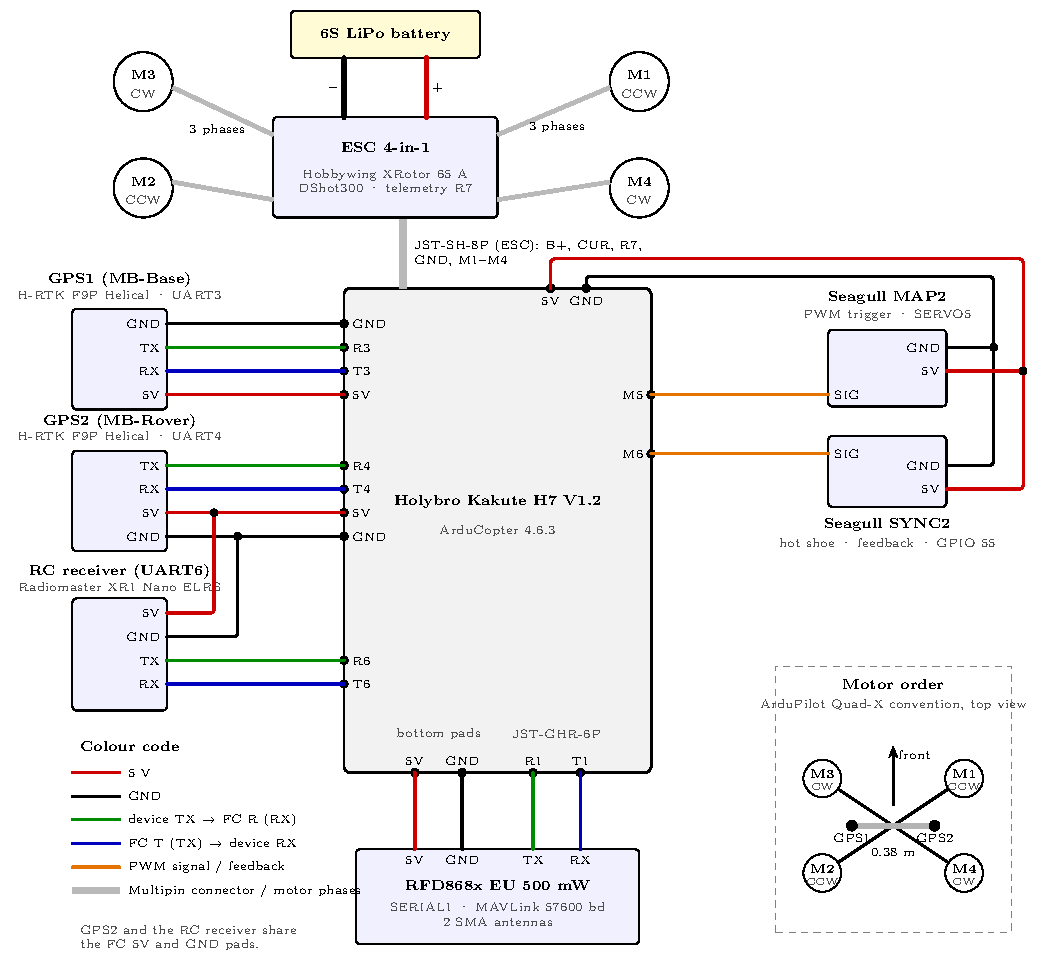
\includegraphics[width=\textwidth]{img/diagrama_connexions_en.pdf}
    \caption{Connection diagram of the drone. The colours follow the legend: green for the TX line of the device towards the RX of the FC and blue for the TX of the FC towards the RX of the device.}
    \label{fig:connexions}
\end{figure}

\begin{table}[H]
    \centering
    \caption{Flight controller connections (Kakute H7 V1.2)}
    \label{tab:connexions}
    \small
    \begin{tabular}{P{3.2cm}P{3.9cm}P{3.5cm}P{2.6cm}}
        \toprule
        Device & FC pads & Function & ArduPilot port \\
        \midrule
        GPS1 (MB-Base) & R3, T3, 5V, GND & UART & \texttt{SERIAL3} \\
        GPS2 (MB-Rover) & R4, T4, 5V, GND & UART & \texttt{SERIAL4} \\
        ELRS receiver & R6, T6, 5V, GND & UART (CRSF) & \texttt{SERIAL6} \\
        RFD868x & R1, T1 (JST-GHR-6P); 5V, GND & UART (MAVLink) & \texttt{SERIAL1} \\
        4-in-1 ESC & JST-SH-8P: B+, CUR, R7, GND, M1--M4 & DShot, voltage, current, telemetry & \texttt{SERIAL7} \\
        Seagull MAP2 & M5; 5V, GND & \emph{trigger} PWM & \texttt{SERVO5} \\
        Seagull SYNC2 & M6; 5V, GND & hot-shoe \emph{feedback} & \texttt{SERVO6} (GPIO 55) \\
        \bottomrule
    \end{tabular}
\end{table}

\subsection{GNSS base}
\label{subsec:muntatge-base}

The base is a compact stack of three boards fixed to one leg of the tripod with clamps (\cref{fig:base}): the ArduSimple simpleRTK2B Pro receiver (with the ZED-F9P), the Raspberry Pi Zero W and the Waveshare UPS HAT with the two 18650 batteries. The BD900 GNSS antenna is mounted levelled, with a ground plane, on the 5/8-inch thread of the survey tripod, at a height of 122~cm in the flight tests.

The connections are (\cref{fig:base-connexions}):
\begin{itemize}
    \item \textbf{Antenna $\rightarrow$ simpleRTK2B Pro:} coaxial cable with SMA connector.
    \item \textbf{simpleRTK2B Pro $\rightarrow$ Raspberry Pi:} one USB-C cable, which carries the data (RTCM3 corrections and receiver configuration) and powers the receiver from the Pi.
    \item \textbf{UPS HAT $\rightarrow$ Raspberry Pi:} only the power pins of the Pi header are connected to the UPS HAT, which powers it from the batteries; there is no communication line between the two.
\end{itemize}

\begin{figure}[H]
    \centering
    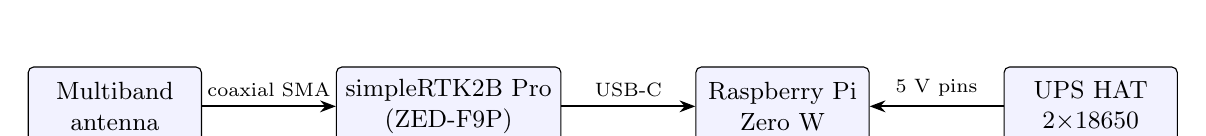
\begin{tikzpicture}[box/.style={draw, rounded corners=2pt, align=center, font=\small, minimum height=10mm, minimum width=22mm, fill=blue!5},
        arr/.style={-{Stealth[length=2mm]}, thick}, node distance=17mm]
        \node[box] (ant) {Multiband\\antenna};
        \node[box, right=of ant] (rtk) {simpleRTK2B Pro\\(ZED-F9P)};
        \node[box, right=of rtk] (pi) {Raspberry Pi\\Zero W};
        \node[box, right=of pi] (ups) {UPS HAT\\2$\times$18650};
        \draw[arr] (ant) -- node[above, font=\scriptsize] {coaxial SMA} (rtk);
        \draw[arr] (rtk) -- node[above, font=\scriptsize] {USB-C} (pi);
        \draw[arr] (ups) -- node[above, font=\scriptsize] {5~V pins} (pi);
    \end{tikzpicture}
    \caption{RTK base connections: antenna, receiver, SBC and power.}
    \label{fig:base-connexions}
\end{figure}

\begin{figure}[H]
    \centering
    \begin{subfigure}[b]{0.43\textwidth}
        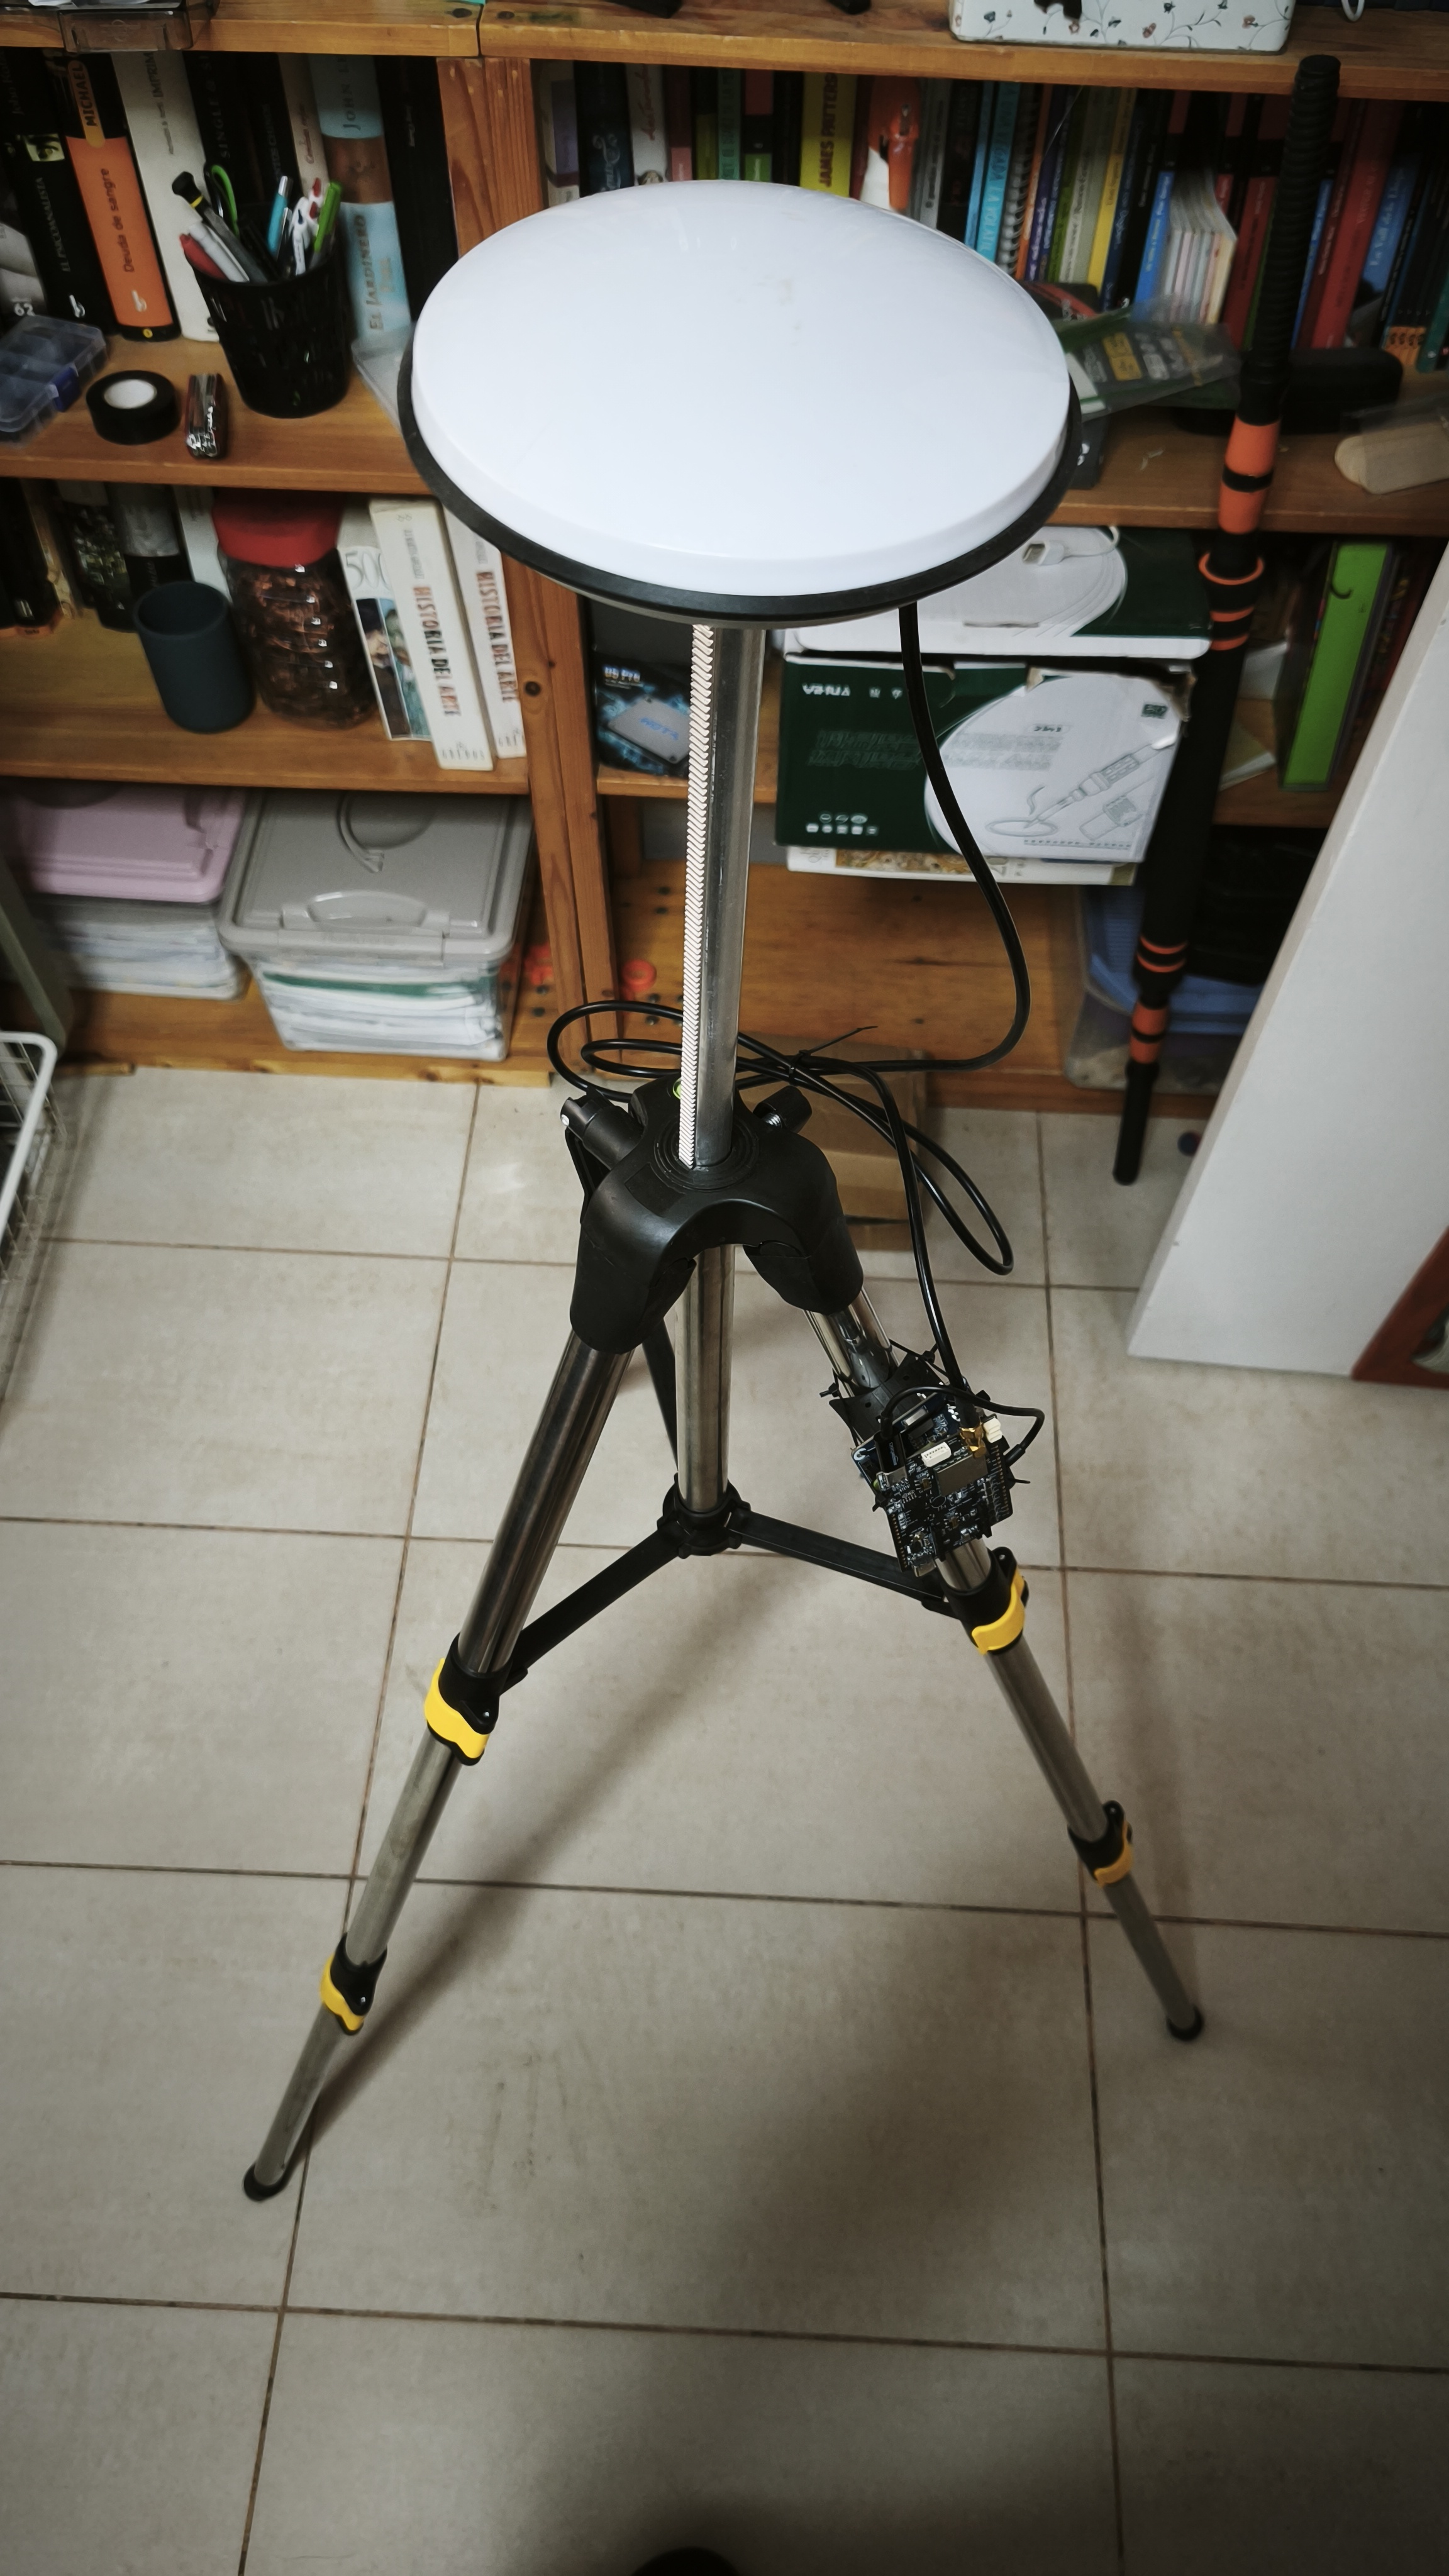
\includegraphics[width=\textwidth]{img/Base_sencera.jpg}
        \caption{Complete base on the tripod.}
    \end{subfigure}
    \hfill
    \begin{subfigure}[b]{0.43\textwidth}
        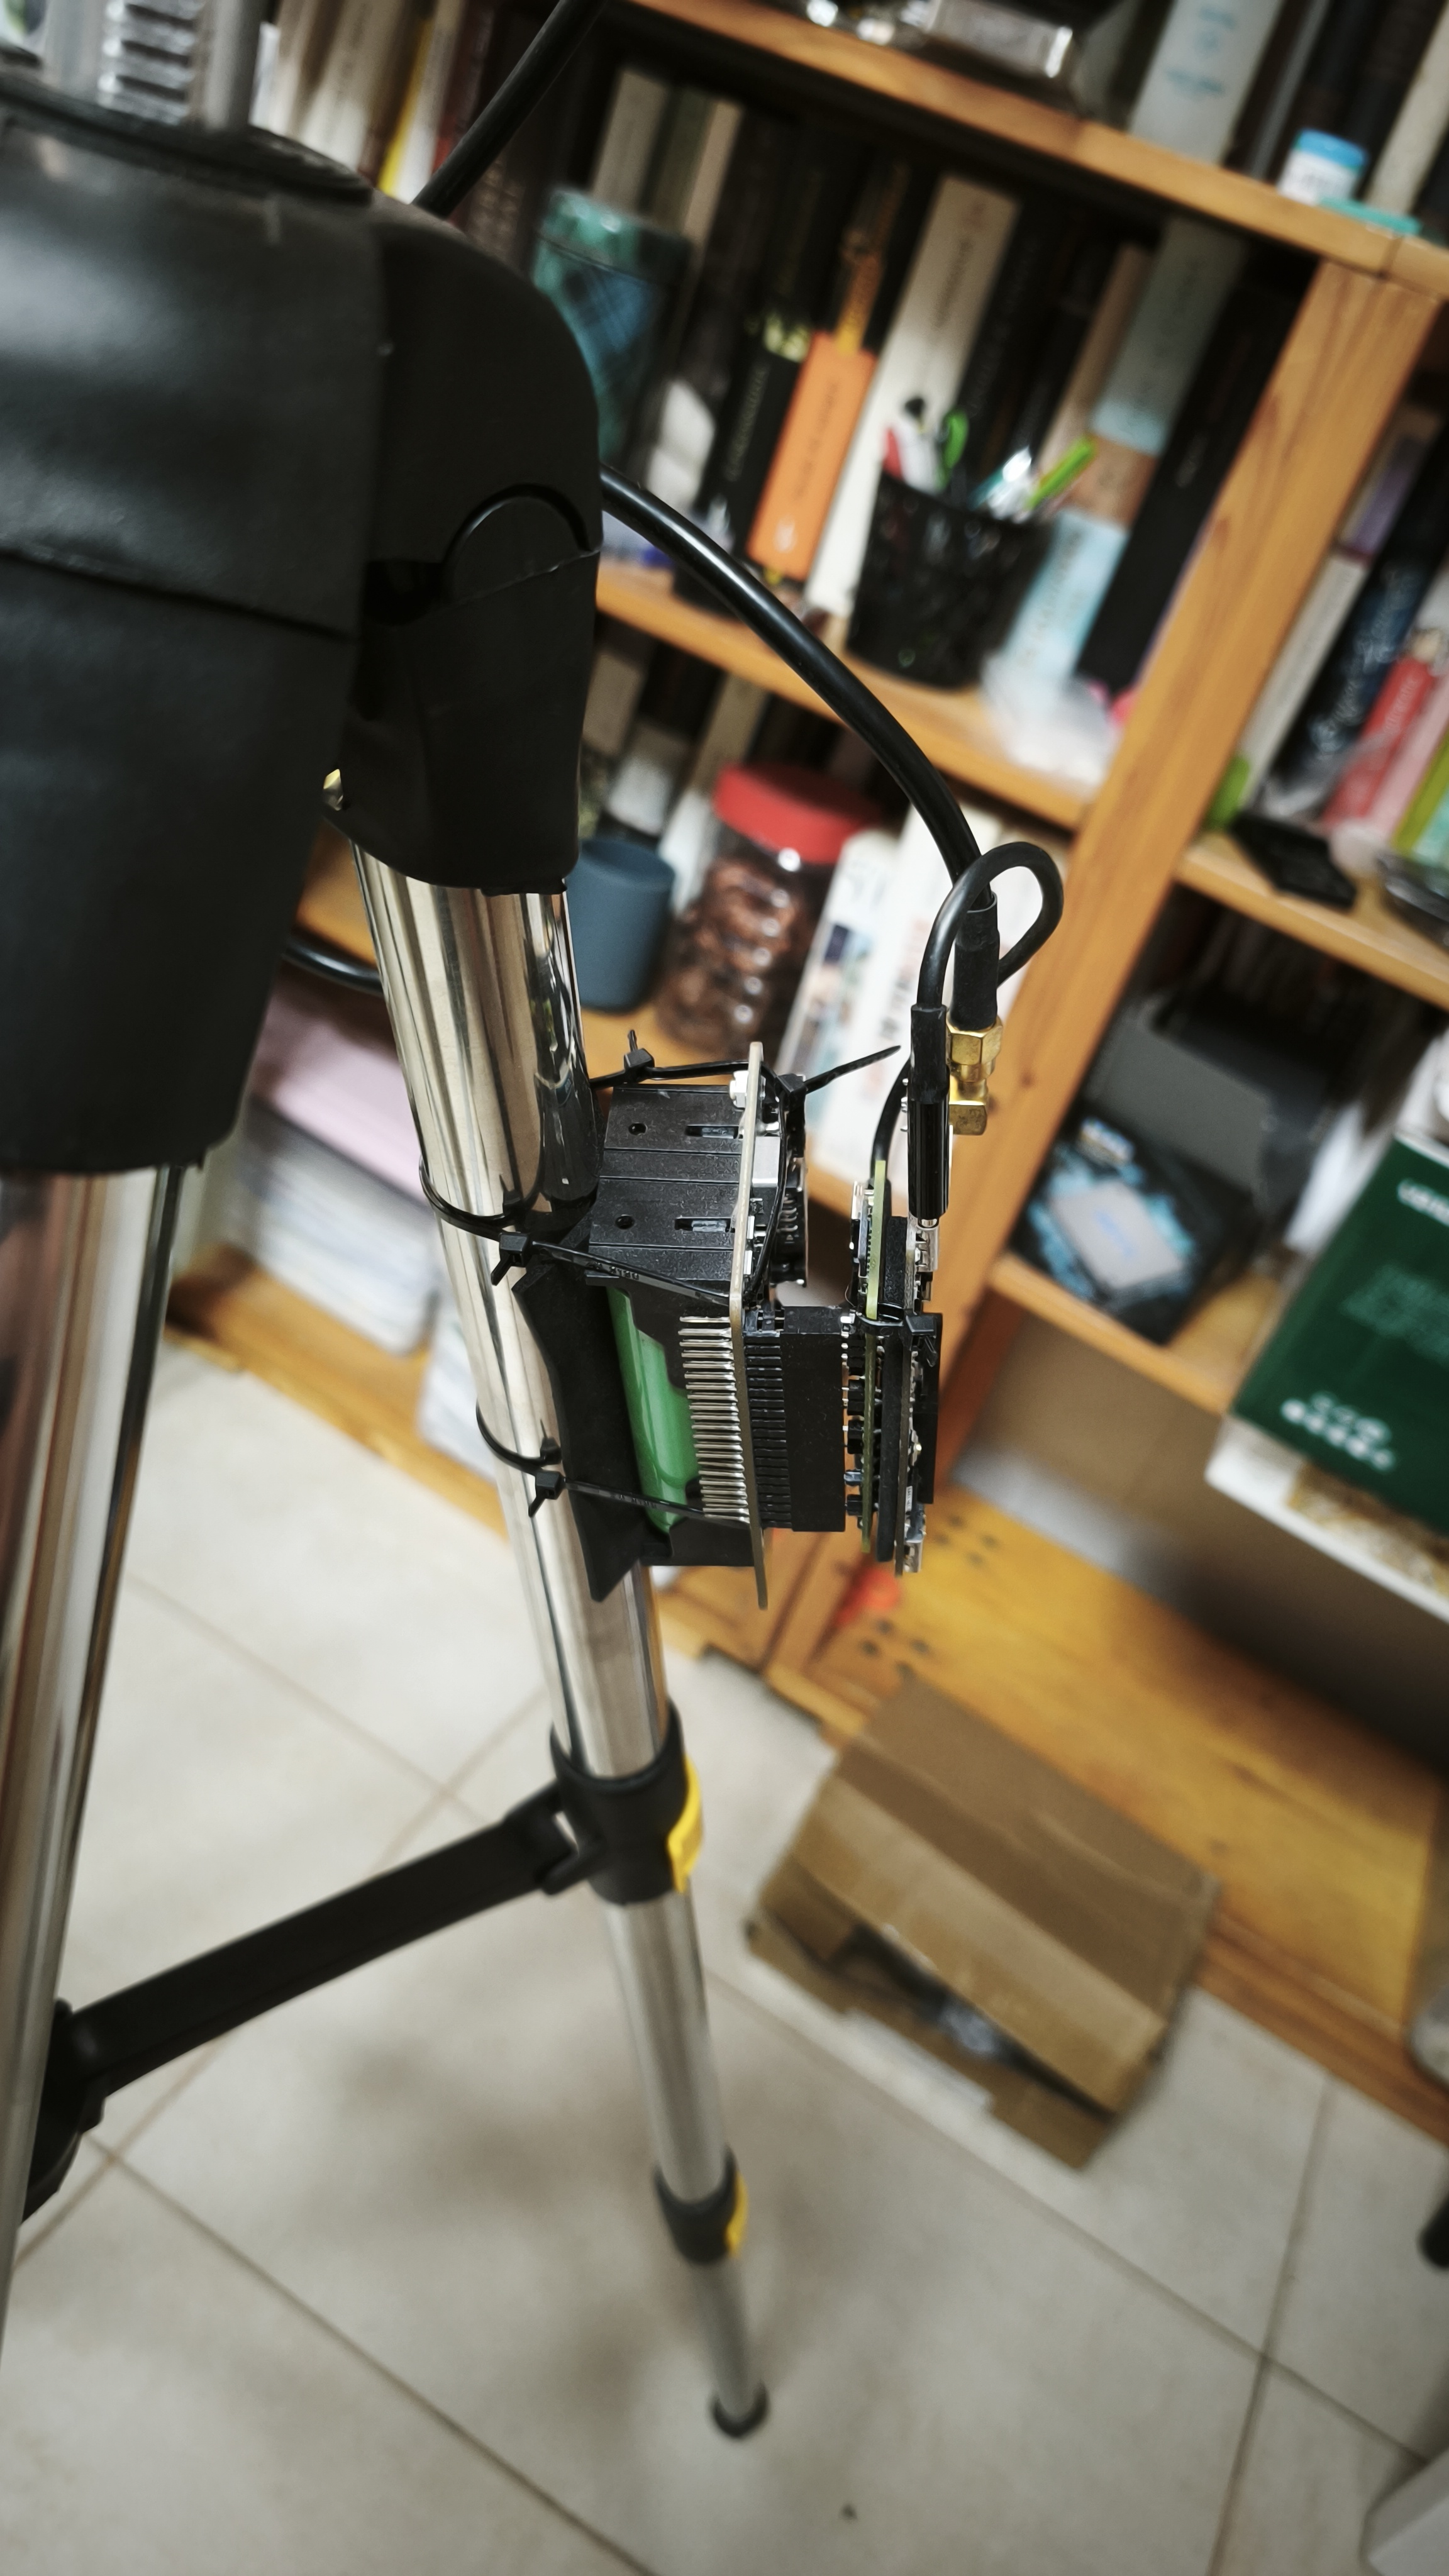
\includegraphics[width=\textwidth]{img/Stack_base.jpg}
        \caption{Base stack fixed to a leg.}
    \end{subfigure}
    \caption{RTK base: multiband antenna on the tripod and stack with the simpleRTK2B Pro, the Raspberry Pi and the UPS HAT.}
    \label{fig:base}
\end{figure}

The procedure for positioning the base and fixing its coordinates is described in \cref{sec:protocol-camp}.

\paragraph{Software and configuration.} The Raspberry Pi runs Raspberry Pi OS (Debian~13, 32-bit). The corrections are distributed by the RTKLIB \texttt{str2str} program (the \texttt{rtklibexplorer} fork, compiled on the Pi itself), run as a \texttt{systemd} service that starts with the board. The service is called \texttt{rtkbase}, but it has no relation to the \texttt{rtkbase} project in the bibliography: it reads the USB serial port of the receiver (115,200~bd) and opens a TCP server on port 5000 that forwards the receiver stream as it comes out (RTCM3 and the UBX navigation messages that it emits on the same port), without NTRIP. Besides forwarding it, the service saves it to a file for the whole session (\cref{sec:protocol-camp}). The GS connects to it with Mission Planner's \emph{RTK/GPS Inject} in \emph{TCP Client} mode, at \texttt{192.168.4.1:5000}.

The WiFi access point (\texttt{BaseRTK}) is managed by NetworkManager in \emph{shared} mode: 2.4~GHz band, channel~6, WPA-PSK, address \texttt{192.168.4.1/24} with DHCP, and it is activated at every boot. PMF (802.11w) must be disabled, because the \texttt{brcmfmac} driver of the Pi does not support it in AP mode.

The ZED-F9P (\emph{firmware} HPG~1.51, protocol~27.50) is configured with \texttt{ubxtool}: NMEA disabled on the USB port, RTCM3 enabled and messages 1005, 1074, 1084, 1094, 1124 and 1230 at 1~Hz. The total stream on port 5000, with the UBX navigation messages that the receiver also emits, was about 15~kbps. The base position is not fixed: the receiver runs a \emph{survey-in} in every session, with 300~s as a minimum and until the precision of the mean is 2~m or better, and the configuration is kept in the \emph{flash} memory of the receiver. Flight tests 5 and 6 used this base and this method, with the antenna at 122~cm.

\textbf{Limitation.} In flight tests 5 and 6 the service only forwarded the stream, without saving it, and the position resulting from the \emph{survey-in} was not noted down; therefore the absolute position of those flights cannot be recovered. Since every session performs a new one, the absolute position of the map has a common error of the order of metres; this shifts the whole map but does not change its relative geometry. Since 27 October 2026 the service saves the stream of every session, so the position can be computed afterwards (\cref{sec:protocol-camp}).

\section{System status}
\label{sec:estat-actual}

The hardware is complete and the system has accumulated about 30~minutes of flight according to the controller counter, spread between the tuning campaign (\cref{chap:proves-vol}) and two photogrammetry flights (\cref{chap:vols-prova}). With the current configuration the drone flies with RTK Fixed on both receivers and valid GNSS \emph{yaw}, and the photographic chain (distance-based triggering, hot-shoe \emph{feedback}, geotagging and processing) is operational end to end. The current limitations --~above all the endurance and the absolute validation with control points~-- are collected in \cref{sec:balanc-vols,sec:autonomia}, and the pending work is in \cref{sec:pendents-proves-vol}.

\chapter{Operation manual and procedures}
\label{chap:manual}

This chapter collects the reference configuration of the system and the working procedure, applicable to any photogrammetry flight. The results obtained with these procedures are presented in \cref{chap:vols-prova}.

\section{GNSS antennas}
\label{sec:antenes-gnss}

\subsection{Drone helical antennas}

The two helical antennas of the \emph{rover} are mounted:
\begin{itemize}
    \item Vertical, parallel to each other, pointing up.
    \item At the highest point of the drone.
    \item With a minimum separation of 10~cm from the VTx, the ESCs and the power cables, to avoid interference.
    \item Without tilt with respect to the vertical axis.
\end{itemize}

\subsection{\emph{Moving baseline} baseline}

The separation between the two helical antennas is \textbf{0.38~m}, on a rigid carbon \emph{bracket} aligned with the Y (lateral) axis of the drone. The \emph{offsets} with respect to the centre of gravity are $Y = \mp 0.19$~m and $Z = -0.10$~m (GPS1 on the left, GPS2 on the right), with $X = 0$ (\cref{tab:params-gps-mb}).

The \emph{heading} precision of a \emph{moving baseline} scales inversely with the baseline length: with 0.38~m a $\sigma$ of the order of $0.5^{\circ}$ is estimated, which must be validated empirically (\cref{sec:validacio}). Any change in the length of the \emph{bracket} requires recalibrating the GNSS \emph{heading}.

\subsection{Base antenna}

Horizontal \emph{patch} antenna with a ground plane, levelled on the survey tripod.

\subsection{Camera timing}

The central pin of the camera \emph{hot shoe} is the \textbf{X-sync} signal: the Seagull SYNC2 fits directly onto it, since the Sony $\alpha$6000 has a \emph{Multi Interface Shoe} compatible with the ISO~518 standard.

\section{FC serial port configuration (Kakute H7)}
\label{sec:ports-serie}

\begin{table}[H]
    \centering
    \caption{Serial port assignment of the Kakute H7}
    \label{tab:ports-serie}
    \begin{tabular}{lllc}
        \toprule
        Port & Function & Baud rate & Protocol \\
        \midrule
        SERIAL0 (USB) & MAVLink2 (configuration) & -- & -- \\
        SERIAL1 (UART1, VTX port) & RFD868x MAVLink & 57600 & 2 \\
        SERIAL2 (UART2) & Internal Bluetooth (occupied) & -- & Disabled \\
        SERIAL3 (UART3) & F9P \#1 -- GPS1 (MB-Base) & 230400 & 5 \\
        SERIAL4 (UART4) & F9P \#2 -- GPS2 (MB-Rover) & 230400 & 5 \\
        SERIAL6 (UART6) & RC ELRS (CRSF) & 420000 & 23 \\
        SERIAL7 (UART7, ESC port) & ESC telemetry & 115200 & 16 \\
        \bottomrule
    \end{tabular}
\end{table}

\section{Camera configuration}
\label{sec:config-camera}

\subsection{Controller parameters}

From ArduPilot 4.5 on, the camera parameters have the prefix \texttt{CAM1\_*} to support multiple cameras; the old documentation and forums still use \texttt{CAM\_*} names.

\begin{table}[H]
    \centering
    \caption{Camera parameters (ArduPilot 4.5 or later)}
    \label{tab:params-camera}
    \begin{tabular}{lP{9.5cm}}
        \toprule
        Parameter & Value / Function \\
        \midrule
        \texttt{SERVO5\_FUNCTION} & 10 (\emph{CameraTrigger}, MAP2 on pad M5) \\
        \texttt{CAM1\_TYPE} & 1 (Servo) \\
        \texttt{CAM1\_DURATION} & 1.0 (in \textbf{seconds}, not ms): the MAP2 in IS-T mode needs commands of 1~s \\
        \texttt{CAM1\_SERVO\_ON} & 1700 (IS-T mode) \\
        \texttt{CAM1\_SERVO\_OFF} & 1500 (inside the MAP2 rest range, 1400--1600) \\
        \texttt{SERVO5\_TRIM} & 1500 \\
        \texttt{CAM1\_TRIGG\_DIST} & 0 in the base configuration; set for each mission (\cref{sec:planificacio-vol}) \\
        \texttt{SERVO6\_FUNCTION} & $-1$ (GPIO for the SYNC2 \emph{feedback}, pad M6) \\
        \texttt{CAM1\_FEEDBAK\_PIN} & 55 \\
        \texttt{CAM1\_FEEDBAK\_POL} & 1 \\
        \bottomrule
    \end{tabular}
\end{table}

The parameter name is \texttt{CAM1\_FEEDBAK\_PIN}, spelled \textbf{without the ``C''} of \emph{feedback} (historical ArduPilot naming). Pin 55 corresponds to the \texttt{SERVO6} pad reassigned as GPIO.

With a manual lens without electronic contacts, the MAP2 must not work in AF-T mode (useless 1~s pre-focus, which adds a constant delay). The diagnosis is detailed in \cref{subsec:problemes-camera}.

\subsection{Camera settings}
\label{subsec:ajust-camera}

\begin{table}[H]
    \centering
    \caption{Sony $\alpha$6000 settings for photogrammetry}
    \label{tab:ajust-camera}
    \begin{tabular}{ll}
        \toprule
        Setting & Value \\
        \midrule
        Exposure mode & M (manual) \\
        Shutter speed & 1/1600~s \\
        Aperture & f/5.6 (ring fixed with tape) \\
        Focus & Manual at infinity (both rings fixed with tape) \\
        ISO & Auto, with a ceiling at 1600 \\
        Drive mode & \emph{Single shot}, JPEG Fine \\
        Shutter & Electronic front curtain enabled \\
        \emph{Release w/o Lens} & Enabled (needed with a lens without contacts) \\
        \bottomrule
    \end{tabular}
\end{table}

The manual lens does not send data to the camera: the EXIF records \texttt{FocalLength=0} and an empty \texttt{LensModel}, and the orientation would depend on the heading (\cref{sec:processament-fotos}). This metadata is rewritten in post-processing.

The camera has no dynamic range to compensate for low light: photographs must be taken with the sun more than 10--15$^{\circ}$ above the horizon (\cref{sec:vol6}).

\subsection{Shutter delay}

The controller trigger command (\texttt{TRIG}) and the actual exposure are separated by $\approx 0.28$~s (\cref{sec:retard-obturador}); at 5~m/s that is $\approx 1.4$~m. For this reason the geotagging uses the position of the \texttt{CAM} message (instant of the hot-shoe \emph{feedback}) when it is available, and compensates with $v\cdot\tau$ when it is not.

\section{\emph{Moving baseline} GPS and \emph{yaw} configuration}
\label{subsec:gps-moving-baseline}

\begin{table}[H]
    \centering
    \caption{\emph{Moving baseline} and GPS-for-yaw parameters}
    \label{tab:params-gps-mb}
    \begin{tabular}{ll}
        \toprule
        Parameter & Value \\
        \midrule
        \texttt{GPS1\_TYPE} & 17 (MB-Base) \\
        \texttt{GPS2\_TYPE} & 18 (MB-Rover) \\
        \texttt{GPS\_AUTO\_CONFIG} & 1 \\
        \texttt{GPS\_DRV\_OPTIONS} & 0 \\
        \texttt{GPS\_INJECT\_TO} & 127 \\
        \texttt{EK3\_SRC1\_POSXY} / \texttt{VELXY} & 3 (GPS) \\
        \texttt{EK3\_SRC1\_YAW} & 2 (GPS yaw) \\
        \texttt{COMPASS\_ENABLE} & 0 (no compass) \\
        \texttt{GPS1\_POS\_X/Y/Z} & $0$ / $-0.19$ / $-0.10$~m \\
        \texttt{GPS2\_POS\_X/Y/Z} & $0$ / $+0.19$ / $-0.10$~m \\
        \texttt{GPS1\_MB\_OFS\_Y} & $-0.38$~m \\
        \bottomrule
    \end{tabular}
\end{table}

\texttt{GPS\_DRV\_OPTIONS} must be 0: the value 1 (use of UART2 for the \emph{moving baseline}) assumes a direct cable between the UART2 ports of the two F9Ps to carry the RTCM stream, which does not exist in this build; with the bit set, the \emph{rover} never reaches RTK Fixed (\texttt{PreArm: GPS[2] yaw not available}). The stream between receivers goes through the flight controller.

\section{Control, battery and safety}
\label{sec:params-control}

\begin{table}[H]
    \centering
    \caption{Control, battery and safety parameters of the reference configuration}
    \label{tab:params-control}
    \small
    \begin{tabular}{ll}
        \toprule
        Parameter & Value \\
        \midrule
        \texttt{FRAME\_CLASS} & 1 (Quad) \\
        \texttt{FRAME\_TYPE} & 1 (X) \\
        \texttt{MOT\_PWM\_TYPE} & 5 (DShot300)~\cite{ardupilot_dshot} \\
        \texttt{ATC\_RAT\_RLL\_P} / \texttt{ATC\_RAT\_PIT\_P} & 0.07 \\
        \texttt{ATC\_RAT\_RLL\_I} / \texttt{ATC\_RAT\_PIT\_I} & 0.07 \\
        \texttt{ATC\_RAT\_RLL\_D} / \texttt{ATC\_RAT\_PIT\_D} & 0.002 \\
        \texttt{ATC\_RAT\_YAW\_P} & 0.10 \\
        \texttt{ATC\_RAT\_YAW\_I} & 0.01 \\
        \texttt{MOT\_THST\_EXPO} & 0.65 \\
        \texttt{MOT\_SPIN\_ARM} & 0.04 \\
        \texttt{MOT\_SPIN\_MIN} & 0.06 \\
        \texttt{MOT\_THST\_HOVER} & 0.225 (learned in flight, \texttt{MOT\_HOVER\_LEARN=2}) \\
        \texttt{BATT\_MONITOR} & 4 (analogue voltage and current) \\
        \texttt{BATT\_VOLT\_MULT} & 10.82 (calibrated) \\
        \texttt{BATT\_AMP\_PERVLT} & 87.73 (calibrated) \\
        \texttt{BATT\_LOW\_VOLT} / \texttt{BATT\_FS\_LOW\_ACT} & 21.6~V / 2 (RTL) \\
        \texttt{BATT\_CRT\_VOLT} / \texttt{BATT\_FS\_CRT\_ACT} & 20.4~V / 1 (Land) \\
        \texttt{BATT\_FS\_VOLTSRC} & 0 (instantaneous voltage) \\
        \texttt{FENCE\_ENABLE} / \texttt{FENCE\_TYPE} & 1 / 7 (altitude, circle and polygon) \\
        \texttt{FENCE\_RADIUS} & 700~m \\
        \texttt{FENCE\_ALT\_MAX} & 120~m \\
        \texttt{WPNAV\_SPEED} & 500~cm/s (5~m/s) in automatic missions \\
        \texttt{FLTMODE1} to \texttt{FLTMODE6} & Stabilize, AltHold, Loiter, Auto, Guided, RTL \\
        \texttt{LOG\_BITMASK} & 196607 \\
        \bottomrule
    \end{tabular}
\end{table}

\section{Pre-flight checklist}
\label{sec:checklist-prevol}

\begin{enumerate}[label=\arabic*.]
    \item Verify that both F9Ps (base and drone) report \texttt{RTK Fixed} before arming, with the correct \emph{fix} type on both receivers (not \texttt{RTK Float} or \texttt{3D Fix}).
    \item Verify that the GNSS \emph{yaw} (\emph{moving baseline}) is valid and consistent with the real \emph{heading} (margin $< 1^{\circ}$).
    \item Check the RFD868x GS$\leftrightarrow$drone link and the reception of RTCM corrections on the drone.
    \item Check the battery level of the drone (voltage per cell) and of the base (UPS).
    \item Check the SD card and the camera battery, and that the settings are those of \cref{tab:ajust-camera}.
    \item Test the trigger with \emph{Trigger Camera Now} and confirm that \texttt{CAM} messages appear (SYNC2 \emph{feedback} active).
    \item Review the assigned flight modes and that the \emph{geofence} is active (\cref{tab:params-control}).
    \item Check in Mission Planner that the EKF3 is healthy (no position or velocity variance warnings), that the HDOP is low (recommended $< 1$ with RTK Fixed) and that there is no pending \emph{prearm} message.
    \item Verify that \texttt{COMPASS\_ENABLE=0} and that there is no compass \emph{prearm error}.
    \item Check the \emph{failsafes}: loss of RC, loss of telemetry, low and critical battery.
    \item Check that the sun is more than 10--15$^{\circ}$ above the horizon and that the flight area and the airspace allow the flight (\cref{sec:normativa}).
\end{enumerate}

\section{Flight planning}
\label{sec:planificacio-vol}

\subsection{GSD calculation}

The \emph{Ground Sample Distance} depends only on the flight height $H$, the sensor size, the focal length $f$ and the image resolution:
\[
\mathrm{GSD}\,\text{(cm/px)} = \frac{H\,\text{(m)} \times \text{sensor width (mm)} \times 100}{f\,\text{(mm)} \times \text{image width (px)}}
\]

With the Sony $\alpha$6000 (APS-C sensor of 23.5~$\times$~15.6~mm, 6000~$\times$~4000~px, pixel size $\approx 3.92$~\textmu m) and the 25~mm TTArtisan lens:
\[
\mathrm{GSD}\,\text{(cm/px)} \approx 0.0157 \times H\,\text{(m)}
\]

\begin{table}[H]
    \centering
    \caption{GSD and coverage per image as a function of height (Sony $\alpha$6000 + TTArtisan 25~mm)}
    \label{tab:gsd-altura}
    \begin{tabular}{ccc}
        \toprule
        Height (m) & GSD (cm/px) & Footprint (m, width $\times$ height) \\
        \midrule
        30 & 0.47 & 28.2 $\times$ 18.7 \\
        50 & 0.78 & 47.0 $\times$ 31.2 \\
        60 & 0.94 & 56.4 $\times$ 37.4 \\
        80 & 1.25 & 75.2 $\times$ 49.9 \\
        100 & 1.57 & 94.0 $\times$ 62.4 \\
        120 & 1.88 & 112.8 $\times$ 74.9 \\
        \bottomrule
    \end{tabular}
\end{table}

The values measured in the flight tests agree with this relation: taking into account the focal length calibrated by the processing (25.72~mm), a GSD of 0.451~cm/px corresponds to a height of 29.6~m (flight planned at 30~m), and a GSD of 0.743~cm/px to 48.9~m (flight planned at $\sim$50~m).

\subsection{Flight parameters}

\begin{table}[H]
    \centering
    \caption{Adopted and recommended flight parameters}
    \label{tab:parametres-vol}
    \begin{tabular}{lP{9cm}}
        \toprule
        Parameter & Value \\
        \midrule
        Flight height & According to the target GSD (\cref{tab:gsd-altura}); 30~m and 50~m in the flight tests \\
        Front / side overlap & 75--77~\% / 65--69~\% in flight 5; 80~\% / 70~\% recommended with complex relief \\
        Speed & 5~m/s (\texttt{WPNAV\_SPEED=500}); limited by \emph{motion blur}: $v_{\max} = \mathrm{GSD}/t_{\text{exposure}}$ \\
        Triggering & By distance (\texttt{CAM1\_TRIGG\_DIST}), with the interval between photos greater than the 1~s of \texttt{CAM1\_DURATION} \\
        Camera orientation & Long side of the sensor along the flight direction \\
        Lighting & Sun more than 10--15$^{\circ}$ above the horizon \\
        \bottomrule
    \end{tabular}
\end{table}

The 80/70~\% overlap percentages are the usual default value in photogrammetry software for precision projects with well-textured terrain; they can be reduced with caution thanks to RTK geotagging, but insufficient overlap still limits the quality of the SfM \emph{matching}. Since \texttt{CAM1\_DURATION=1.0} sets a minimum interval of about 1~s between triggers, at 5~m/s the distance between photos must be at least 5~m (\cref{subsec:autonomia-altura}).

\section{Field protocol}
\label{sec:protocol-camp}

\subsection{Positioning the base}
\begin{enumerate}[label=\alph*)]
    \item Tripod on a stable point with a clear 360$^{\circ}$ sky, away from walls, metal roofs and vehicles; measure the antenna height (122~cm in the flight tests).
    \item Switch on the Pi and wait about 30~s for the \texttt{BaseRTK} network to appear; connect the GS to it.
    \item Restart the \emph{survey-in} to erase the mean of the previous session and wait until it is valid, from the PC connected to \texttt{BaseRTK} and inside the \texttt{base\_rtk} folder: \texttt{python base\_rtk.py survey}. The command shows the duration, the observations and the mean error as it goes, and ends when the \emph{survey-in} is valid (minimum 300~s and mean error, \texttt{meanAcc}, of 2~m or better) or after 20~min (\texttt{--minuts N} changes the limit). While it lasts, the \texttt{rtkbase} service is stopped and port 5000 does not serve; it restarts by itself at the end, also if the SSH connection drops or Ctrl-C is pressed.
    \item If it does not become valid, the mean stalls because of \emph{multipath} or sky obstruction: improve the antenna location, do not extend the wait. The receiver keeps the \emph{survey-in} running, and \texttt{python base\_rtk.py survey --estat} queries it without restarting it.
    \item When the \emph{survey-in} is valid, the command automatically saves the ECEF position (\texttt{meanX/Y/Z}) and the final \texttt{meanAcc} to \texttt{survey.txt}, inside the active session on the Pi. It is the only record of the base position for that session, and it is downloaded with the log (see ``Session log'' below).
\end{enumerate}

While the \emph{survey-in} is not valid, the stream does not carry message 1005 (base position) and the drone cannot reach RTK Fixed. The base position is therefore that of the \emph{survey-in}, with an error of the order of metres that shifts the whole session (\cref{subsec:efecte-surveyin}). To state absolute positions it will be necessary to reuse a fixed position recorded at the same point, or to correct the offset of each session with a PPP solution from its observation log.

\paragraph{Session log.} The \texttt{rtkbase} service saves the receiver stream to files while forwarding it on port 5000, for the whole session: \texttt{str2str} has two outputs, \texttt{tcpsvr://:5000} and \texttt{file:///home/arnau/logs/actual/base\_\%Y\%m\%d\_\%h\%M.rtcm3::S=1}. Each start of the service opens a new \emph{session}, a folder \texttt{/home/arnau/logs/sNNNN/} (\texttt{actual} points to the one in progress), and a file is created inside it every hour (\texttt{::S=1}). The file names carry the UTC time of the Pi, and the date is unreliable, because the Pi has no real-time clock or internet: the valid time is the GNSS time inside the data. A service restart or a power cut opens a new session, except for what \texttt{survey} does, which continues in the same one. The log is the same stream as the port, about 7~MB per hour, with the RTCM3 observations (pseudorange, phase and C/N0 of the four systems), message 1005 once the \emph{survey-in} is valid and the UBX navigation messages that the receiver emits on the same port. It carries no ephemerides, which must be taken from a nearby reference station, nor Doppler.

At the end of the session the log is downloaded before switching off the base, from the PC connected to \texttt{BaseRTK}, with \texttt{python base\_rtk.py baixa} (the last session) or \texttt{python base\_rtk.py baixa N} (session \texttt{N}; \texttt{python base\_rtk.py llista} shows the existing ones, with size and hours). The command joins the hourly files of the session into a single one, \texttt{base\_sNNNN.rtcm3}, checks its size and, if there are \emph{survey-in} notes, also downloads \texttt{base\_sNNNN\_survey.txt}. \texttt{-o folder} says where they are left, and nothing is deleted from the Pi. The file can be converted to RINEX with \texttt{convbin -r rtcm3} to compute afterwards the session position with a PPP solution or relative to a reference station. This computation has not yet been done with any log.

The Pi disk holds about 3,500~h of log and there is no automatic deletion: sessions that are no longer needed are deleted by hand with \texttt{python base\_rtk.py esborra N} or \texttt{esborra --abans N}. The command asks for confirmation and never deletes the active session. The tools and their installation are in the \texttt{base\_rtk} folder, with its \texttt{README.md}.

\subsection{Verifying the \emph{moving baseline}}
\begin{enumerate}[label=\alph*)]
    \item Measure the real vector between the two antennas.
    \item Check the GNSS \emph{yaw} against the real \emph{heading} (margin $< 1^{\circ}$).
\end{enumerate}

\subsection{Flight}
\begin{enumerate}[label=\alph*)]
    \item Base in \texttt{Fixed} $\rightarrow$ the GS injects RTCM into the drone.
    \item Arm \textbf{only} with RTK Fixed on both F9Ps and valid \emph{yaw}.
    \item Fly the planned \emph{grid} in Auto mode.
    \item Download the FC \emph{logs} (\texttt{.bin}) and the photographs from the SD card.
\end{enumerate}

\subsection{Post-processing}
\begin{enumerate}[label=\alph*)]
    \item Pair each photograph with its \texttt{CAM} (or \texttt{TRIG}) message from the \emph{log} and rewrite the EXIF (\cref{sec:processament-fotos}).
    \item Generate the geotag file with the per-photo precision.
    \item Process with ODX/WebODM (\cref{sec:processament}) and generate orthomosaic, DSM and point cloud.
\end{enumerate}

\section{Ground control points (GCP)}
\label{sec:gcp}

The precision of the final product can only be stated with independently measured points. Since the base runs a \emph{survey-in} in every session, the \textbf{coordinate frame} of the points is as important as their precision. The planned protocol is:
\begin{itemize}
    \item Targets well distributed over the whole area, including the corners and the centre, marked with a high-contrast pattern recognisable in the photograph: at least five control points and, separately, ten check points (\cref{subsec:pla-precisio}).
    \item Position of each target measured with RTK against \textbf{the same base and the same session} as the flight, with an expected precision of 1--2~cm. This way the points and the \emph{geotags} share the \emph{survey-in} offset and it cancels in the comparison. If they are measured with a total station or another base, a transformation must be fitted before comparing; otherwise the RMSE is dominated by the metre-level base error.
    \item Separate control points (used in the adjustment) from check points (which do not take part in it), and compute the H/V RMSE of the latter.
\end{itemize}

\pendent{No target has yet been deployed and no control point measured: this is the planned protocol, not a result. It is the task that unlocks absolute precision.}

\section{Processing (\emph{Structure from Motion} and PPK)}
\label{sec:processament}

Photogrammetric processing is done with the ODX 3.8.3 engine (WebODM 3.3.0, NodeODX 2.3.1) on a PC with an i5-10400F, 32~GB of RAM and an RTX~2060. A flight of 118 photographs takes about 42~minutes. The options that depart from the defaults are: orthophoto resolution of 1~cm/px, DEM resolution of 2~cm/px, high point-cloud quality, DSM generation, \emph{auto-boundary}, COG, glTF and EPT \emph{point cloud}. The detail of each processing run is in \cref{chap:vols-prova}.

As an alternative or complement to real-time RTK, \textbf{PPK} post-processing with RTKLIB is contemplated, from the raw \texttt{UBX} recordings of the base and the drone, which gives a positioning solution independent of the quality of the RTK link during the flight.

\pendent{PPK has not yet been applied to any flight: the current processing runs use the real-time RTK positions of the controller.}

\section{Quality control and validation criteria}
\label{sec:validacio}

\subsection{Effect of the \emph{survey-in} on validation}
\label{subsec:efecte-surveyin}

With the \emph{survey-in} the base computes its position as the mean of autonomous positions, without corrections, and broadcasts it in message 1005. The error of this position is transmitted entirely to the \emph{rover}~\cite{ublox_f9p_im}: the whole session is shifted by the same vector, which is of the order of metres (the acceptance criterion of the protocol is a \texttt{meanAcc} of $\leq 2$~m). In contrast, the \emph{relative} position with respect to the base is barely affected: the baseline-length error is that of the base multiplied by the baseline and divided by the distance to the satellites ($\sim 2\cdot 10^{7}$~m), about 0.02~mm with a base shifted by 2~m and a 200~m baseline.

\begin{itemize}
    \item \textbf{Not affected} (can be validated without an absolute reference): the accuracy of the RTK baseline, the repeatability of the \emph{rover}, the \emph{heading} and the internal geometry of the product (shape and scale).
    \item \textbf{Affected:} the absolute position of the map, the comparability between sessions and any comparison with an external reference. Since every session performs a new \emph{survey-in}, two maps of the same place are shifted from each other by the order of metres. The base antenna height (122~cm) enters the elevation with weight 1:1.
\end{itemize}

There are three ways, not mutually exclusive, to recover the absolute position: reuse a fixed position recorded at the same point; measure a known point with the same base and correct its offset; or compute the session position by PPP from the base log and apply the correction vector to the whole product. The latter is feasible in principle with the RTCM stream already generated, which contains MSM observations (1074, 1084, 1094, 1124) convertible to RINEX with RTKLIB (\texttt{convbin}); this must be verified, as well as that the session lasts enough hours for a centimetre-level PPP.

\subsection{Precision test plan}
\label{subsec:pla-precisio}

\begin{table}[H]
    \centering
    \caption{Precision test plan with \emph{survey-in} and current status}
    \label{tab:validacio}
    \footnotesize
    \begin{tabular}{P{0.8cm}P{4.9cm}P{2.8cm}P{2.6cm}P{2.4cm}}
        \toprule
        Test & Procedure & Reference frame & Criterion & Status \\
        \midrule
        T1 & Record \texttt{NAV-SVIN} (\texttt{meanX/Y/Z}, \texttt{meanAcc}) in every session and, in samples, compare it with the PPP solution of the same place & --- & Informative: documents the offset & \textbf{Pending}; not recorded in flights 5 and 6 \\
        T2 & Static \emph{rover} at three distances (e.g.\ 10, 50 and 100~m): RTK base$\rightarrow$\emph{rover} vector against an independent measurement (total station or distance meter and level) & Relative to the base (independent of the \emph{survey-in}) & $< 2$~cm H, $< 3$~cm V & \textbf{Pending} \\
        T3 & Static repeatability: 10--15~min on a point; standard deviation H/V and percentage of RTK Fixed & Relative & Consistent with 0.01~m + 1~ppm & \textbf{Pending} \\
        T4 & \emph{Heading}: GNSS \emph{yaw} against a bearing measured with a total station, in several orientations & Independent of the base & $\sigma < 0.5^{\circ}$ & \textbf{Pending}; \emph{yaw} valid in all flights \\
        T5 & Photogrammetric product: RMSE of the check points, with and without control points, reporting the number of points & Same frame as the \emph{geotags} (same base and session) & $< 3$~cm H, $< 5$~cm V & \textbf{Pending}; internal consistency: reprojection 0.90~px, model--GPS CE90 0.59~m \\
        T6 & Absolute precision: apply the base PPP vector and check against a known geodetic mark & External frame (EPSG:32631) & To be defined (limited by the PPP) & \textbf{Pending}; requires the base log \\
        \bottomrule
    \end{tabular}
\end{table}

The comparison with a DJI P4 RTK reference \emph{dataset} only makes sense after T6, because it needs an absolutely georeferenced map.

On the number of points: with only five, the uncertainty of the RMSE is large. Edition 2 of the ASPRS standard asks for a minimum of 30 check points to state a product precision, and admits a smaller number in small UAS projects if the report declares it~\cite{asprs2023}. For that reason a minimum of ten check points is recommended, in addition to the control points, always reporting the number.

The internal-consistency indicators (reprojection error, difference between the model and the GPS positions of the photos) measure the coherence of the processing, \textbf{not the precision}: they do not replace T2--T6. Until these are done, no absolute or centimetre-level precision is claimed.

\section{Export of results}
\label{sec:exportacio}

Each processing run delivers, in the EPSG:32631 coordinate system (UTM 31N), the following products: GeoTIFF orthophoto (1~cm/px at 30~m), GeoTIFF DSM (2~cm/px), dense point cloud (LAZ and EPT), textured models (OBJ and GLB) and a PDF report with the processing statistics.

\section{Drone maintenance}
\label{sec:manteniment}

\subsection{Before each flight}
\begin{itemize}
    \item Visual inspection of the \emph{frame}, the arms and the \emph{standoffs}: cracks or mechanical play.
    \item Propellers without cracks or deformation, balanced and with the collars well tightened.
    \item XT60/XT90 and JST-GH connectors without play or signs of heating.
    \item Helical antennas well fixed, vertical and without damage to the \emph{baseline} \emph{bracket}.
    \item Battery condition (swelling, voltage per cell) and enough charge for the flight plan.
    \item Camera SD card with enough free space and correctly formatted.
\end{itemize}

\subsection{Periodic maintenance}
\begin{itemize}
    \item Check the tightening torque of motors and arms every few outings.
    \item Check the condition of the motor bearings (noise, play on the shaft).
    \item Update the ArduPilot \emph{firmware} and the F9P receivers only in a controlled way, verifying parameter compatibility before and after.
    \item Periodic verification of the GNSS \emph{heading} against a known reference, to detect mechanical drift of the \emph{bracket}.
    \item Cleaning of contacts and connectors, especially after flying in humid or dusty environments.
    \item LiPo battery maintenance cycles: storage at resting voltage, no discharge below the manufacturer's threshold, and withdrawal of any \emph{pack} that has suffered a \emph{crash}.
\end{itemize}

\section{Regulations and safety}
\label{sec:normativa}

This section is informative and does not constitute legal advice. The EASA regulatory framework for self-built drones is in transition; the current status must be verified before each flight campaign~\cite{easa_open_category}.

\subsection{Drone classification}

This UAV is \textbf{self-built} (\emph{privately built}): it does not come from a ready-to-assemble \emph{kit} sold as a single product, but from individual components. According to EASA, a self-built drone \textbf{cannot carry a class C0--C4 mark}, and therefore is limited, within the \emph{Open} category, to subcategory \textbf{A3} (far from people and built-up areas), with a maximum weight of 25~kg~\cite{easa_open_category}.

Derived practical requirements:
\begin{itemize}
    \item Registration as a drone operator with the competent aeronautical authority (in Spain, AESA) and visible identification of the registration number on the aircraft.
    \item A1/A3 pilot certificate (online training and exam) as a minimum; the operator holds it.
    \item Flight exclusively in subcategory A3: minimum horizontal distance of 150~m from residential, commercial, industrial or recreational areas, and away from people not involved in the operation.
    \item Check of the airspace and local restrictions (\emph{geo-awareness} zones, NOTAM, proximity to airports) before each flight.
    \item Third-party liability insurance, recommended (mandatory in many cases depending on weight and use).
\end{itemize}

Under the transitional rules, self-built drones without a class mark may operate under the inherited regime (by weight) until 1 January 2027. EASA is developing a permanent regime for self-built drones, roughly equivalent to class C4 (subcategory A3, $<25$~kg, pilot with an A1/A3 certificate)~\cite{easa_open_category}.

\subsection{Operational safety}

\begin{itemize}
    \item Do not fly with RTK Float or without a valid GNSS \emph{fix} if the mission depends on centimetre-level precision (it also reduces the quality of the EKF3 position estimate).
    \item Always define a \emph{geofence} and \emph{failsafe} actions for low battery and link loss.
    \item Maintain visual contact (VLOS) unless the corresponding authorisation for BVLOS is held.
    \item Basic risk assessment of the flight area: obstacles, power lines, third parties and weather (wind, rain).
\end{itemize}

\section{Lines of continuation}
\label{sec:treball-futur}

\begin{itemize}
    \item Absolute validation with control and check points (\cref{sec:gcp}).
    \item Endurance improvement: change of the propulsion group and Li-ion battery (\cref{sec:autonomia,sec:propulsor}).
    \item Configuration of the harmonic \emph{notch} filter and Autotune.
    \item Migration to UM982: a single module with native \emph{heading}, less wiring and less consumption.
    \item LiDAR integration (Livox Mid-360) for dense vegetation.
    \item Multispectral camera for precision agriculture.
    \item Own carrier PCB (F9P + SBC + UPS integrated).
    \item Publishing corrections to a community NTRIP network (Centipède~\cite{centipede} or rtk2go).
\end{itemize}

\section{Reference projects}
\label{sec:referencies}

\begin{itemize}
    \item \texttt{rtkbase} (Stefal) -- base software~\cite{rtkbase}.
    \item SparkFun RTK Express -- KiCad design and \emph{firmware}~\cite{sparkfun_rtk_express}.
    \item \texttt{jacobjhansen/RTCM-Pi} -- PPP workflow~\cite{rtcm_pi}.
    \item Centipède -- community NTRIP network in Europe~\cite{centipede}.
    \item ArduPilot -- \emph{moving baseline} and GPS-for-yaw~\cite{ardupilot_moving_baseline}.
\end{itemize}


% =====================================================
% PART II — FLIGHT TESTS
% =====================================================
\part{Flight tests and tuning}
\chapter{Flight tests and tuning}
\label{chap:proves-vol}

This chapter collects the flight-test and tuning campaign carried out between August and October 2026, before operating in \emph{surveys} (\cref{chap:vols-prova}). It records the incidents found in the flight control, the RTK GPS, the camera module and the propulsion group, the causes identified and the changes applied to solve them.

\begin{table}[H]
    \centering
    \caption{Flight sessions of the campaign}
    \label{tab:sessions-vol}
    \small
    \begin{tabular}{llP{8.3cm}}
        \toprule
        Date & Session & Result \\
        \midrule
        6 August & Control tuning & Severe oscillation; \emph{crash} \\
        8 August & Control tuning & Two correct flights; \emph{crash} when changing the orientation \\
        10 August & GPS test & Motor failure in flight; \emph{crash}; \emph{moving baseline} error \\
        27 August & Four flights & Four clean flights, RTK Fixed 100~\% \\
        4 September & \emph{Grid} mission & Cut by the \emph{geofence}; battery collapse \\
        8 October & Flight test 5 & 118 photos; orthomosaic and DSM (\cref{sec:vol5}) \\
        13 October & Flight test 6 & Two flights at dawn; one usable batch (\cref{sec:vol6}) \\
        20 October & 8-inch propellers & Two aborted arms (\cref{subsec:propulsor-8in}) \\
        \bottomrule
    \end{tabular}
\end{table}

\section{Initial controller configuration}
\label{sec:config-inicial}

The first review of the controller parameter file detected and corrected the following problems:

\begin{itemize}
    \item \texttt{FRAME\_CLASS} unassigned (now Quad, X).
    \item GPS position \emph{offsets} (\texttt{GPS1\_POS\_*} / \texttt{GPS2\_POS\_*}) at zero; measured with respect to the centre of gravity (\cref{tab:params-gps-mb}).
    \item \texttt{EK3\_SRC1\_YAW} pointing to the compass: changed to GPS \emph{yaw}.
    \item Compass enabled with no sensor connected: disabled.
    \item \texttt{BATT\_MONITOR} at 0: changed to analogue voltage and current.
    \item \texttt{MOT\_PWM\_TYPE} at PWM: changed to DShot300.
    \item All flight modes at Stabilize: assigned Stabilize, AltHold, Loiter, Auto, Guided and RTL.
    \item \texttt{SERVO9} assigned to \emph{Scripting1} with no real use: disabled.
\end{itemize}

\section{Chronology of incidents}
\label{sec:cronologia-incidents}

\subsection{6 August -- Severe oscillation and \emph{crash}}

\emph{Wobbling} in the arms when raising throttle, with repeatable lateral drift. In the \emph{log}, the \emph{rate} loop changed sign in 65~\% of the samples, with errors of up to $301^{\circ}$/s. It ended with \texttt{Crash: Disarming: AngErr=51>30}.

Causes identified:
\begin{itemize}
    \item Drone heavily overpowered (\texttt{MOT\_THST\_HOVER=0.20}, \emph{hover} at 20~\%) with default PIDs designed for a \emph{hover} of 35--50~\%.
    \item Motors saturating at the minimum because of a too high \texttt{MOT\_SPIN\_MIN}.
    \item \texttt{MOT\_THST\_EXPO=0.8}.
    \item No \emph{notch} filter, with vibrations of 44~m/s\textsuperscript{2} and 42 \emph{clips}.
    \item A \texttt{SAVE\_TRIM} done in flight had contaminated \texttt{AHRS\_TRIM\_X}.
\end{itemize}

\subsection{8 August -- \emph{Crash} due to an orientation change}

The first two flights of the day went well (oscillation down from 65~\% to 3--6~\%, zero \emph{clips}). On the third, when setting \texttt{AHRS\_ORIENTATION} from 4 to 0, the drone flipped in 0.4~s with the controller saturated opposite to the rotation: pure positive feedback.

The real problem was not the orientation but the polarity of channel 2: \emph{roll} responded correctly, only \emph{pitch} was inverted. It was solved by inverting the \emph{elevator} on the Radiomaster.

\subsection{10 August -- \emph{Crash} due to motor failure}

Stable \emph{hover} for 10~s, then sudden loss. Motor M3 was commanded to 2000 with no effect; the current dropped from 16~A to 8.9~A, the voltage recovered and the vibrations fell just before the exit: unmistakable signature of a motor stopped in flight.

The same day it was identified that \texttt{GPS\_DRV\_OPTIONS=1} prevented the \emph{moving baseline}: this value assumes a direct cable between the UART2 ports of the two F9Ps, which does not exist in this build. The \emph{rover} never reached RTK Fixed, hence the \texttt{PreArm: GPS[2] yaw not available} (\cref{subsec:gps-moving-baseline}).

\subsection{27 August -- Four clean flights}

First session without incidents. GPS[0] and GPS[1] at 100~\% RTK Fixed, GPS \emph{yaw} available in all samples, vibrations of 11--16~m/s\textsuperscript{2} and zero \emph{clips} in the four flights.

\subsection{4 September -- Mission cut and \emph{crash} due to battery}

\textbf{Flight 1:} the mission was aborted at \emph{waypoint} 25 of 87 by a \emph{geofence} \emph{breach}. The initial radius of 300~m was insufficient for the new field (farthest \emph{waypoint} at 566~m; 41 of the 87 outside the radius). The photos came out blurred.

\textbf{Flight 2:} battery collapse. From 22.4~V to 8~V in 25~seconds with only 5~A of load. The counter showed 213~mAh consumed from a 4000 \emph{pack}, impossible: the current sensor was badly calibrated. The \emph{sag} went from 0.63~V to 1.79~V in 18~seconds: internal resistance tripled, a cell dying. The \emph{failsafes} acted correctly (RTL at 758~s, Land at 763~s), but there was no energy left to land.

\subsection{4--13 September -- Camera problems}
\label{subsec:problemes-camera}

In flight 1: 121 trigger commands, only 33 confirmed exposures, all with a constant delay of 1.16~s. In flight 2: 50 commands, zero photos.

A first diagnosis attributed the EXIF readings \texttt{FNumber=0}, \texttt{FocalLength=0} and \texttt{LensModel} set to \texttt{"----"} to a failure of the electrical contacts. In fact it is the normal behaviour of a manual TTArtisan 25~mm f/2, which has no electronic contacts.

Real causes:
\begin{itemize}
    \item The MAP2 was in AF-T mode (\texttt{CAM1\_SERVO\_ON=1300}), which does a useless 1~s pre-focus with a manual lens: hence the constant delay.
    \item \texttt{CAM1\_SERVO\_OFF=1100} outside the rest range expected by the MAP2 (1400--1600).
    \item \texttt{CAM1\_DURATION=0.1} too short for the MAP2 to read the command (IS-T mode wants 1.0~s).
    \item \emph{Release w/o Lens} possibly disabled, which blocks the shutter with a lens without contacts.
    \item Slow shutter and active autofocus in flight 1 (cause of the blurred photos).
    \item The \emph{grid} configuration assumed 20~mm when the real lens is 25~mm: all the computed overlap was wrong.
\end{itemize}

Once the changes were applied, flight 2 of test 6 gave 110 trigger commands, 110 \emph{feedback} confirmations and 110 photographs (\cref{sec:vol6}).

\section{Parameter changes applied}
\label{sec:canvis-aplicats}

\subsection{Control (6 August)}

\begin{table}[H]
    \centering
    \caption{Control tuning after the oscillation of 6 August}
    \label{tab:canvis-control}
    \begin{tabular}{lll}
        \toprule
        Parameter & From & To \\
        \midrule
        \texttt{ATC\_RAT\_RLL\_P} / \texttt{PIT\_P} & 0.135 & 0.070 \\
        \texttt{ATC\_RAT\_RLL\_I} / \texttt{PIT\_I} & 0.135 & 0.070 \\
        \texttt{ATC\_RAT\_RLL\_D} / \texttt{PIT\_D} & 0.0036 & 0.0020 \\
        \texttt{ATC\_RAT\_YAW\_P} & 0.18 & 0.100 \\
        \texttt{MOT\_THST\_EXPO} & 0.8 & 0.65 \\
        \texttt{MOT\_SPIN\_ARM} & 0.10 & 0.04 \\
        \texttt{MOT\_SPIN\_MIN} & 0.15 & 0.06 \\
        \texttt{ATC\_RAT\_*\_FLTD} / \texttt{FLTT} & 20 & 10 \\
        \texttt{AHRS\_TRIM\_X} / \texttt{Y} & contaminated & recalibrated ($\approx 0$) \\
        \texttt{LOG\_BITMASK} & 180222 & 196607 \\
        \bottomrule
    \end{tabular}
\end{table}

\subsection{GPS}

\begin{table}[H]
    \centering
    \caption{GPS configuration changes after the incident of 10 August}
    \label{tab:canvis-gps}
    \begin{tabular}{lll}
        \toprule
        Parameter & From & To \\
        \midrule
        \texttt{GPS\_DRV\_OPTIONS} & 1 & 0 \\
        \texttt{GPS1\_POS\_Y} / \texttt{GPS2\_POS\_Y} & 0 & $-0.19$ / $+0.19$ \\
        \texttt{GPS1\_POS\_Z} / \texttt{GPS2\_POS\_Z} & 0 & $-0.10$ / $-0.10$ \\
        \bottomrule
    \end{tabular}
\end{table}

\subsection{Safety and battery}

\begin{table}[H]
    \centering
    \caption{Safety (\emph{failsafes}, \emph{geofence}) and battery changes after 4 September}
    \label{tab:canvis-seguretat}
    \begin{tabular}{lll}
        \toprule
        Parameter & From & To \\
        \midrule
        \texttt{BATT\_FS\_LOW\_ACT} & 0 & 2 (RTL) \\
        \texttt{BATT\_FS\_CRT\_ACT} & 0 & 1 (Land) \\
        \texttt{BATT\_LOW\_VOLT} / \texttt{CRT\_VOLT} & -- & 21.6 / 20.4 \\
        \texttt{BATT\_AMP\_PERVLT} & uncalibrated & 87.73 \\
        \texttt{BATT\_VOLT\_MULT} & uncalibrated & 10.82 \\
        \texttt{FENCE\_ENABLE} & 0 & 1 \\
        \texttt{FENCE\_RADIUS} & 300 & 700 \\
        \texttt{WPNAV\_SPEED} & 1000 & 500 \\
        \texttt{SR1\_*} (RFD telemetry) & 0 & active \\
        \bottomrule
    \end{tabular}
\end{table}

\subsection{Camera}
\label{subsec:canvis-camera-pendents}

\begin{table}[H]
    \centering
    \caption{Camera changes derived from the diagnosis of \cref{subsec:problemes-camera}}
    \label{tab:canvis-camera}
    \begin{tabular}{lll}
        \toprule
        Parameter & Before & Now \\
        \midrule
        \texttt{CAM1\_SERVO\_ON} & 1300 (AF-T) & 1700 (IS-T) \\
        \texttt{CAM1\_SERVO\_OFF} & 1100 & 1500 \\
        \texttt{CAM1\_DURATION} & 0.1 & 1.0 \\
        \texttt{SERVO5\_TRIM} & 1100 & 1500 \\
        \bottomrule
    \end{tabular}
\end{table}

The physical camera setup is in \cref{tab:ajust-camera}. The Mission Planner \emph{grid} is planned with the real 25~mm focal length.

\section{Measured progression}
\label{sec:progressio-mesurada}

\begin{table}[H]
    \centering
    \caption{Progression of the flight metrics over the campaign}
    \label{tab:progressio}
    \begin{tabular}{lcccccc}
        \toprule
        Metric & 6 Aug & 8 Aug & 27 Aug & 4 Sep & 8 Oct & 13 Oct \\
        \midrule
        \emph{Roll rate} sign changes & 65~\% & 3--6~\% & 8--9~\% & stable & -- & -- \\
        VibeZ max.\ (m/s\textsuperscript{2}) & 44 & 40 & 11--16 & 14--18 & 10.8 & 14.1--15.7 \\
        \emph{Clips} & 42 & 0--29 & 0 & 0 & 0 & 0 \\
        GPS[0] RTK Fixed & -- & -- & 100~\% & 100~\% & 100~\% & -- \\
        GPS[1] RTK Fixed & -- & 0~\% & 100~\% & 100~\% & 100~\% & -- \\
        \emph{Hover throttle} & 20~\% & 20~\% & 45~\% & 45~\% & -- & -- \\
        \bottomrule
    \end{tabular}
\end{table}

The 8 and 13 October columns correspond to flight tests 5 and 6 (for 6, the range covers both flights). Vibration was computed from the \texttt{VIBE} messages of the \emph{logs}, only with the motors running; the median VibeZ is 3.9~m/s\textsuperscript{2} in flight 5 and 5.0--5.3~m/s\textsuperscript{2} in flight 6. Dashes are metrics that have not been computed for these flights.

\section{Endurance and performance improvement}
\label{sec:autonomia}

Endurance is the biggest limitation of the current platform. \emph{Hover} at 45~\% \emph{throttle} (\cref{tab:progressio}) is stable, but the system carries 520~g of APS-C camera with a propulsion group that was not chosen for efficiency (\cref{sec:propulsor}): it works, but the price is flight time. This section compares the improvement options by cost and expected gain; the propulsion group is detailed in the next section.

\begin{table}[H]
    \centering
    \caption{Options to improve endurance and performance per battery}
    \label{tab:opcions-autonomia}
    \small
    \begin{tabular}{P{3.4cm}P{1.7cm}P{2.5cm}P{5.9cm}}
        \toprule
        Option & Cost & Gain & Comment \\
        \midrule
        Fly at 45--50~m & €0 & $+60$~\% area per battery & The \emph{grid} must be recomputed with the 25~mm focal length; it also relaxes the trigger rate (\cref{subsec:autonomia-altura}). \\
        \emph{Notch} + Autotune & €0 & 5--10~\% & See \cref{subsec:autonomia-notch}. \\
        6S2P Li-ion battery & $\sim$€120 & $\times 1.7$ flight time & Molicel P42A or P45B. Avoid Samsung 50E: 10~A per cell is little for a \emph{hover} of $\sim$17~A (\cref{subsec:autonomia-liion}). \\
        8-inch propellers (current motors) & $\sim$€15 & $+12$--$18$~\% endurance & Uses the margin of the 1100~KV motors (\cref{sec:propulsor}). \\
        400--500~KV motors + 12--13-inch propellers & $\sim$€140 & $\sim\times 1.8$--$2$ flight time & The current 500~mm \emph{frame} already allows it; FC, F9P, radio and camera stay (\cref{subsec:autonomia-frame}). \\
        Li-ion + new motors and propellers & $\sim$€260 & 30+~min & The real jump to a \emph{survey} platform. \\
        \bottomrule
    \end{tabular}
\end{table}

\subsection{Raising the flight height (zero cost)}
\label{subsec:autonomia-altura}

The width of the strip photographed in each pass is proportional to the height ($H \cdot 23.5/25$~m with the current sensor and optics, \cref{tab:gsd-altura}). Flying higher covers the same area with fewer passes and therefore less flight time: the gain is directly the ratio of heights. Flight test 5 was flown at 30~m, so going up to 48~m gives $+60$~\% of area per battery (45~m: $+50$~\%; 50~m: $+67$~\%), as is already done in flight test 6 (50~m).

The cost is GSD: at 50~m it is still $\approx 0.8$~cm/px, below the 1--2~cm/px range considered sufficient for precision surveying, so there is room to go up without losing quality.

Going up also relaxes the trigger rate. With 80~\% front overlap and 70~\% side overlap, the distance between photos and between lines grows with height (assuming the short side of the sensor along the route); at the current speed of 5~m/s (\texttt{WPNAV\_SPEED=500}, \cref{tab:canvis-seguretat}), the interval between triggers is that of \cref{tab:ritme-dispar}.

\begin{table}[H]
    \centering
    \caption{\emph{Grid} spacing and trigger interval as a function of height (25~mm, 80/70~\%, 5~m/s)}
    \label{tab:ritme-dispar}
    \small
    \begin{tabular}{ccccc}
        \toprule
        $H$ (m) & GSD (cm/px) & Between photos (m) & Between lines (m) & Interval (s) \\
        \midrule
        30 & 0.47 & 3.7 & 8.5 & 0.75 \\
        40 & 0.63 & 5.0 & 11.3 & 1.00 \\
        45 & 0.71 & 5.6 & 12.7 & 1.12 \\
        50 & 0.78 & 6.2 & 14.1 & 1.25 \\
        \bottomrule
    \end{tabular}
\end{table}

The new \texttt{CAM1\_DURATION=1.0} (\cref{tab:canvis-camera}) forces a minimum interval of about 1~s between commands, so at 40~m and 5~m/s it is already at the limit, and at 30~m (0.75~s between photos) it would not be viable with these overlaps. At 45--50~m there is a small margin, and in addition fewer photos are fired in total (less data to process).

\subsection{\emph{Notch} and Autotune}
\label{subsec:autonomia-notch}

The harmonic \emph{notch} filter (configured from the frequency measured with FFT in \emph{hover} and from the ESC RPM) removes the vibration noise from the control loop. With less noise, the controller does not have to spend authority correcting it and the motors run cleaner. Autotune, once the \emph{notch} is well set, allows raising gains without reintroducing oscillation. The estimated gain is modest (5--10~\%), but it costs nothing.

\subsection{6S2P Li-ion battery}
\label{subsec:autonomia-liion}

A 6S2P \emph{pack} of 21700 cells of 4200~mAh (Molicel P42A) has $\approx 8.4$~Ah at $\approx 21.6$~V nominal, about 181~Wh, compared with the $\approx 89$~Wh of the current 6S 4000~mAh LiPo: more than double the energy. Since the \emph{pack} also weighs more, the net flight-time gain is estimated at $\times 1.7$ and not $\times 2$.

The choice of cell is critical for current. According to most distributors (figures that must be checked against the manufacturer's \emph{datasheet} before buying), the P42A (and the P45B) supports 45~A continuous per cell, while the Samsung 50E only 9.8~A. With a \emph{hover} of $\sim$17~A shared between two cells in parallel, each cell carries $\sim$8.5~A: the 50E would already be at 87~\% of its limit just hovering, with no margin for manoeuvres or for a large \emph{sag}, while the P42A works at 19~\%.

\subsection{Large propellers and low-KV motors}
\label{subsec:autonomia-frame}

This is the dominant factor: the efficiency of a multirotor depends on the disc loading (thrust per unit of swept area), so larger propellers directly reduce the power needed in \emph{hover}. The current 500~mm-between-axes \emph{frame} already admits propellers of up to 13~inches, but the 1100~KV motors are not compatible with them: the change has two levels (8-inch propellers with the current motors, or 12--13~inches with 400--500~KV motors). The derivation, the KV--propeller compatibilities and the measurement protocol are developed in \cref{sec:propulsor}. The electronics (FC, the two F9Ps, the radio and the camera) stay unchanged.

\section{Propulsion group optimisation}
\label{sec:propulsor}

\subsection{Starting point and initial constraint}
\label{subsec:propulsor-inicial}

The initial propulsion configuration of the prototype was:

\begin{table}[H]
    \centering
    \caption{Initial propulsion configuration}
    \label{tab:propulsor-inicial}
    \begin{tabular}{ll}
        \toprule
        Element & Specification \\
        \midrule
        \emph{Frame} & Quad X, 500~mm between axes \\
        Motors & Pilotix 2808, 1100~KV \\
        Propellers & HQProp 7 $\times$ 4 $\times$ 3 (three-blade) \\
        Battery & LiPo 6S 4000~mAh \\
        AUW & 2.2~kg (including the photographic payload) \\
        \bottomrule
    \end{tabular}
\end{table}

The choice of the 7-inch propellers \textbf{did not respond to a design criterion but to availability}: they were propellers from a previous build and were reused to put the prototype in the air at no additional cost. This decision was reasonable in the commissioning phase --~what had to be validated then was the RTK architecture, the \emph{moving baseline} and the camera triggering chain, not efficiency~-- but it remained as technical debt once the system was operational. The later review of the propulsion group is the subject of this section.

\subsection{Diagnosis}
\label{subsec:propulsor-diagnostic}

The analysis of the flight logs and the \emph{frame} geometry revealed two inconsistencies.

\textbf{The \emph{frame} is underused.} In an X configuration, the distance between adjacent motors is the diagonal divided by $\sqrt{2}$:
\[
d_{\text{adjacent}} = \frac{500}{\sqrt{2}} \approx 354~\text{mm}
\]
This allows propellers of up to $\sim$330~mm (13~inches) with no overlap between discs. With 7-inch propellers (178~mm), \textbf{only 30~\% of the available disc area} was being used.

\textbf{The thrust-to-weight ratio is excessive for a mapping platform.} The \texttt{MOT\_THST\_HOVER} parameter, learned in flight, is 0.23: \emph{hover} is held with a low fraction of the available thrust. The resulting thrust-to-weight ratio is $\sim$3.1:1 when 2:1 is enough for a mapping platform. A propulsion group oversized in thrust and undersized in disc area works far from its point of maximum efficiency.

Both symptoms point to the same thing: \textbf{the propeller diameter is the limiting factor}.

\subsection{Theoretical basis}
\label{subsec:propulsor-teoria}

The induced power that a rotor needs to sustain a thrust $T$ in hover is given by momentum theory:
\[
P_i = T \sqrt{\frac{T}{2\rho A}}, \qquad A = \frac{\pi D^2}{4}
\]
where $\rho$ is the air density and $A$ the disc area. Since $P_i \propto 1/\sqrt{A} \propto 1/D$, \textbf{increasing the diameter directly reduces the power needed}. The relevant quantity is the disc loading $T/A$: the lower, the more efficient the rotor.

Applied to the case ($T = 550$~g per motor, $\rho = 1.225$~kg/m\textsuperscript{3}):

\begin{table}[H]
    \centering
    \caption{Ideal induced power in \emph{hover} as a function of propeller diameter}
    \label{tab:potencia-induida}
    \small
    \begin{tabular}{lcccc}
        \toprule
        Propeller & Disc area & Disc loading & $P_i$ per motor & $P_i$ total \\
        \midrule
        7 inches & 248~cm\textsuperscript{2} & 22.2~kg/m\textsuperscript{2} & 50.8~W & 203~W \\
        \textbf{8 inches} & \textbf{324~cm\textsuperscript{2}} & \textbf{17.0~kg/m\textsuperscript{2}} & \textbf{44.5~W} & \textbf{178~W} \\
        13 inches & 857~cm\textsuperscript{2} & 6.4~kg/m\textsuperscript{2} & 27.4~W & 109~W \\
        \bottomrule
    \end{tabular}
\end{table}

The step from 7 to 8~inches reduces the ideal induced power by \textbf{12.4~\%}; the step to 13~inches, by \textbf{46~\%}.

These values are the theoretical limit: the real power includes the profile drag of the blades (typical figure of merit 0.65--0.75) and the efficiency of the motor-ESC assembly. In practice the total gain approaches that of the induced component, which is dominant in hover.

\subsection{Motor--propeller compatibility constraint}
\label{subsec:propulsor-kv}

The disc area cannot be increased freely: the KV of the motor must correspond to the diameter of the propeller. A motor with too high a KV for its propeller works at high torque and few revolutions, far from its point of maximum efficiency, and the aerodynamic gain is lost in electrical and thermal losses.

\begin{table}[H]
    \centering
    \caption{Suitable KV as a function of propeller diameter (6S voltage)}
    \label{tab:kv-compatibilitat}
    \begin{tabular}{lcc}
        \toprule
        Propeller & Suitable KV & Current motor (1100~KV) \\
        \midrule
        7 inches & 1200--1400 & slightly low \\
        \textbf{8 inches} & \textbf{950--1100} & \textbf{optimal match} \\
        9 inches & 800--900 & $\sim$25~\% above \\
        12--13 inches & 400--500 & incompatible \\
        \bottomrule
    \end{tabular}
\end{table}

This constraint explains a counter-intuitive result: \textbf{9-inch propellers would perform worse than 8-inch ones} despite having more disc area, because the KV mismatch penalises the motor more than the disc contributes. The 8-inch propellers are therefore the optimum attainable \textbf{without replacing the motors}.

\subsection{Propeller selection}
\label{subsec:propulsor-seleccio}

Once the diameter was fixed, the available options were evaluated.

\textbf{Number of blades.} At equal diameter and thrust, a two-blade propeller is aerodynamically more efficient than a three-blade one. However, the 8-inch offer for multirotors is mostly three-blade, and the available two-blade ones (APC 8$\times$4.5MR and MRP) have a \textbf{speed limit of $\sim$13,100~min\textsuperscript{$-1$}}. With 1100~KV on 6S (24,400~min\textsuperscript{$-1$} unloaded) this limit could be exceeded in full-throttle manoeuvres --~gusts, recoveries, \emph{failsafe} climbs~--, with a risk of blade breakage. With a photographic payload underneath, the reliability criterion prevails over the marginal efficiency gain.

\textbf{Decision:} the three-blade configuration is kept and a \textbf{glass-fibre-reinforced nylon} propeller is adopted, sized for the speeds usual in high-speed multirotors.

\begin{table}[H]
    \centering
    \caption{8-inch candidate propellers}
    \label{tab:helix-candidates}
    \small
    \begin{tabular}{llcP{6.4cm}}
        \toprule
        Candidate & Pitch & Mass & Notes \\
        \midrule
        \textbf{HQProp LR8X4.2X3} & 4.2 in. & -- & \emph{Long Range} range, designed for efficient cruise with a payload \\
        HQProp MacroQuad 8$\times$4$\times$3 & 4.0 in. & 12.8~g & Bore 15.7~mm, hole 9.5/5~mm (rings not included) \\
        Gemfan 8040-3 & 4.0 in. & -- & Equivalent, wide availability in Europe \\
        \bottomrule
    \end{tabular}
\end{table}

The \textbf{HQProp LR8X4.2X3} is chosen. The pitch/diameter ratio (0.53) is lower than that of the initial configuration (0.57), which favours performance in hover and slow cruise, which is the working regime of a mapping mission.

\subsection{Checks before mounting}
\label{subsec:propulsor-verificacions}

\begin{itemize}
    \item \textbf{Shaft diameter:} 5~mm, or adapter rings.
    \item \textbf{Camera field of view:} going from 7 to 8~inches adds 12.7~mm of radius per propeller. It must be confirmed that the blades do not enter the frame with the 25~mm lens in a nadir mount.
    \item \textbf{Ground clearance} with the current landing gear.
    \item \textbf{ESC current margin:} the current per motor decreases as the diameter increases, so no review of the sizing is needed.
\end{itemize}

\subsection{First test with 8-inch propellers (20 October)}
\label{subsec:propulsor-8in}

The first test with the 8-inch propellers ended in two aborted arms. In both, the pattern was the same: Loiter mode, take-off ramp with motor output of 43--55~\%, 25--31~A, voltage above 23.85~V, and the \emph{log} ends between 0.1 and 0.5~s later, with no \emph{failsafe} or error recorded.

The controller stays calm and the four motors are symmetric (within $\pm 2$~\%). The vibration, however, is much higher than in the previous flights: 15--35~m/s\textsuperscript{2} in the first arm and 32--92~m/s\textsuperscript{2} (with \emph{clipping}) in the second, against a median of 3--5~m/s\textsuperscript{2} and a maximum of $\sim$16~m/s\textsuperscript{2} in the previous flights. The raw IMU shows a tonal vibration --~narrow peaks at the rotation frequency, which grow with acceleration (127--134~Hz $\rightarrow$ 159--173~Hz)~-- and not a broadband one, which points to propeller imbalance (1$\times$ component) rather than rubbing. The parameters and filters were not touched for the propeller change. The exact cause of the \emph{log} cut has not been determined; the working hypothesis is propeller imbalance, which must be ruled out by balancing them before repeating the test.

\subsection{Control retuning}
\label{subsec:propulsor-control}

The change of diameter modifies the rotational inertia and the control authority, so the angular-rate loop gains stop being valid. After mounting it is necessary to:

\begin{enumerate}[label=\arabic*.]
    \item \textbf{Redo the harmonic \emph{notch} filter.} The fundamental frequency of the motors drops as the diameter increases. Procedure: \texttt{INS\_RAW\_LOG\_OPT = 9}, a 60--90~s flight with varied manoeuvres, analysis with ArduPilot's \emph{Filter Review} tool.
    \item \textbf{Reduce the P and D gains} of the \emph{roll} and \emph{pitch} axes as a conservative starting point, and run \textbf{Autotune} axis by axis once the flight is verified to be stable.
\end{enumerate}

\subsection{Measurement protocol}
\label{subsec:propulsor-mesura}

To quantify the real gain, a controlled comparison protocol is established. \textbf{Prerequisite: calibration of the current and voltage sensor} (\texttt{BATT\_AMP\_PERVLT}, \texttt{BATT\_VOLT\_MULT}), without which the energy measurements are not valid. This requirement is already met (\cref{tab:canvis-seguretat}).

\textbf{Identical conditions between tests:} same grid, height, cruise speed, payload, battery mass and wind conditions ($< 3$~m/s).

\textbf{Variables to record in each test:}

\begin{table}[H]
    \centering
    \caption{Variables to record per test}
    \label{tab:variables-mesura}
    \begin{tabular}{ll}
        \toprule
        Variable & Source \\
        \midrule
        Energy consumed (mAh) & \texttt{BAT.CurrTot} in the log \\
        Armed time (s) & \texttt{ARMED} / \texttt{DISARMED} marks \\
        Average consumption (A) & \texttt{BAT.Curr} \\
        Average power (W) & \texttt{BAT.Curr} $\times$ \texttt{BAT.Volt} \\
        Efficiency (g/W) & AUW $\div$ average power \\
        \texttt{MOT\_THST\_HOVER} & parameter learned in flight \\
        Area covered (ha) & mission planning \\
        \bottomrule
    \end{tabular}
\end{table}

\textbf{Derived metrics:} mAh per minute, \textbf{hectares per battery} (the relevant quantity for the operator) and g/W (the relevant quantity for engineering).

\begin{table}[H]
    \centering
    \caption{Propulsion group comparison: initial configuration (measured in flight test 6, flight 2) and 8-inch propellers (pending)}
    \label{tab:resultats-propulsor}
    \begin{tabular}{lccc}
        \toprule
        Metric & 7 $\times$ 4 $\times$ 3 (initial) & 8 $\times$ 4.2 $\times$ 3 & Change \\
        \midrule
        Energy until \emph{failsafe} (mAh) & 2,012 & pending & \\
        Time until \emph{failsafe} (min) & 10.6 & pending & \\
        Average consumption (A) & 22 & pending & \\
        Average power (W) & $\approx 500$ & pending & \\
        Efficiency (g/W) & $\approx 4.4$ & pending & \\
        \texttt{MOT\_THST\_HOVER} & 0.23 & pending & \\
        Hectares per battery at 50~m & 3.1 & pending & \\
        \bottomrule
    \end{tabular}
\end{table}

\noindent\textit{Prior estimate: $+12$--$18$~\% endurance.}

\smallskip
\noindent The values in the initial column come from flight 2 of flight test 6 (\cref{sec:vol6}), measured with the current sensor already calibrated. The power is the product of the average current and an average voltage of $\sim$22.5~V. Both flights of test 6 end by low-battery \emph{failsafe} when only 47--50~\% of the nominal capacity has been used, because of the voltage drop under load (\cref{sec:vol6}): the usable endurance is limited by voltage, not by energy.

\subsection{Line of continuity}
\label{subsec:propulsor-continuitat}

The 8-inch configuration exhausts the margin available with the current motors. Making full use of the 500~mm \emph{frame} requires replacing the motor group:

\begin{table}[H]
    \centering
    \caption{Propulsion group configurations and estimated endurance}
    \label{tab:continuitat-propulsor}
    \small
    \begin{tabular}{lccc}
        \toprule
        Configuration & Disc loading & Theoretical $P_i$ & Estimated endurance \\
        \midrule
        7 inches (initial) & 22.2~kg/m\textsuperscript{2} & 203~W & 10--11~min \\
        8 inches & 17.0~kg/m\textsuperscript{2} & 178~W & 12--13~min \\
        \textbf{12--13 inches, 450--500~KV motors} & \textbf{6.4~kg/m\textsuperscript{2}} & \textbf{109~W} & \textbf{18--22~min} \\
        \bottomrule
    \end{tabular}
\end{table}

Candidates: Sunnysky X3108 480~KV or T-Motor MN3110 470~KV with 12 $\times$ 4 or 13 $\times$ 4.4 propellers. The resulting thrust-to-weight ratio ($\sim$2.6:1) remains adequate for mapping operation. The arm mounting pattern must be verified: 28xx-series motors usually mount with a 16 $\times$ 16~mm pattern and 31xx with 19 $\times$ 19 or 25 $\times$ 25~mm.

Combined with a \textbf{6S2P Li-ion} \emph{pack} of high-discharge cells (Molicel P42A or P45B, 206~Wh/kg versus the 143~Wh/kg of the current LiPo; \cref{subsec:autonomia-liion}), the projected endurance exceeds 30~minutes.

\subsection{Conclusion}

The initial 7-inch configuration was a decision to make use of material at hand, adequate for the commissioning phase but suboptimal once the system became operational. The later analysis identifies the propeller diameter as the limiting factor of efficiency and establishes two improvements of very different cost:

\begin{itemize}
    \item \textbf{Change to 8-inch propellers} ($\sim$€15): uses the margin that the current motors allow.
    \item \textbf{Change of motor group to 12--13~inches} ($\sim$€140): uses the existing \emph{frame} and almost doubles the endurance.
\end{itemize}

Neither requires modifying the RTK architecture, the photographic chain or the flight software, which remain intact.


\section{Status and pending work}
\label{sec:pendents-proves-vol}

\subsection{Resolved during the campaign}
\begin{itemize}
    \item Stable control and \emph{moving baseline} with RTK Fixed at 100~\% on both receivers. Vibration, measured in the log (\texttt{VIBE} message) with the motors running, has a median of 2--5~m/s\textsuperscript{2} and a maximum of 10.8~m/s\textsuperscript{2} in flight test 5 and 18.7~m/s\textsuperscript{2} in 6, with no \emph{clipping} (\cref{tab:progressio}).
    \item Current and voltage sensor calibrated (\texttt{BATT\_AMP\_PERVLT}, \texttt{BATT\_VOLT\_MULT}); the current sensor read below the real value, which hid the real consumption until the battery collapse of 4 September.
    \item Camera trigger chain operational: IS-T trigger, hot-shoe \emph{feedback} on pin 55 (110 of 110 exposures confirmed in flight 2 of test 6) and \emph{grid} planned with the real 25~mm focal length.
    \item Lateral \emph{baseline} with GPS1 on the left (\texttt{GPS1\_POS\_Y=$-0.19$}), with valid GNSS \emph{yaw}.
\end{itemize}

\subsection{Pending: tests and improvements}
\begin{itemize}
    \item Harmonic \emph{notch}: measure the frequency with FFT in \emph{hover} and configure it in mode 3 (ESC RPM); the \emph{IMU batch sampler} is already active (\texttt{INS\_LOG\_BAT\_MASK=1}). Verify \texttt{SERVO\_BLH\_POLES=14} against the real RPM, because the \emph{notch} depends on it. Autotune afterwards.
    \item 6S2P Li-ion battery and, if more endurance is needed, change of motor group (\cref{sec:autonomia}).
    \item Ground control and check points, measured with the same base and session as the flight, to state a precision (\cref{sec:gcp}).
    \item Compute by PPP the offset of the first session with a base log (the service already saves the stream and the \emph{survey-in} position of every session, \cref{sec:protocol-camp}) and check that the conversion to RINEX works (\cref{subsec:efecte-surveyin}).
    \item Repeat the field flight (flight test 6) with the sun more than 10--15$^{\circ}$ above the horizon (\cref{sec:vol6}).
    \item Precision test plan T1--T6 (\cref{tab:validacio}), with the GNSS \emph{heading} and the accuracy of the RTK baseline; application of PPK (\cref{sec:processament}).
\end{itemize}


% =====================================================
% PART III — PHOTOGRAMMETRY FLIGHTS
% =====================================================
\part{Photogrammetric results}
\chapter{Photogrammetry test flights}
\label{chap:vols-prova}

This chapter presents the two photogrammetry flights made with the complete system once the control and the GPS were stabilised (\cref{chap:proves-vol}): flight test 5, at 30~m over a park, and flight test 6, at 50~m over a field. Both ran the whole chain --~planning, automatic flight with RTK, geotagging, processing and export~-- and serve to quantify its behaviour, in particular the shutter delay (\cref{sec:retard-obturador}).

\section{Processing chain}
\label{sec:cadena-processat}

\subsection{Capture}

The mission is a \emph{grid} in Auto mode at 5~m/s with distance-based triggering. The MAP2 fires the camera by PWM and the SYNC2, on the hot shoe, returns the real instant of the exposure to the controller, which records it as a \texttt{CAM} message in the \emph{log} (the trigger command is recorded as \texttt{TRIG}). The position of each message is that of the EKF3, with RTK Fixed and GNSS \emph{yaw}.

\subsection{Photograph post-processing}
\label{sec:processament-fotos}

The photographs from the camera cannot be processed as they come out:
\begin{itemize}
    \item \textbf{Orientation.} The EXIF orientation tag of the Sony $\alpha$6000 depends on the heading (the camera points at nadir), while the pixels are always 6000~$\times$~4000. It is normalised to \emph{Orientation}=1 in a copy: only the tag changes, the pixels are not touched.
    \item \textbf{Optics.} The manual lens does not record focal length, model or aperture: they are rewritten (TTArtisan 25~mm, equivalent to 38~mm, f/5.6).
    \item \textbf{Position.} Each photograph is paired with its \emph{log} message (\texttt{CAM} or \texttt{TRIG}), the GPS tags are written into it and a geotag file is generated with the per-photo precision: 0.5~m on straight flight, 1.5~m in turns and 0.3~m vertically.
    \item \textbf{Clock.} The camera clock is off by about 9~h with respect to UTC: pairing is done by order (flight 5) or by instant (flight 6), not by the EXIF time.
\end{itemize}

The scripts that perform these steps, the flight \emph{logs}, the corrected photographs, the geotag files and the results of each processing run are archived with SHA-256 checksums, so that each result can be regenerated from the source data.

\subsection{Reconstruction}

Reconstruction is done with ODX 3.8.3 (\cref{sec:processament}). Orthophoto, DSM, point cloud and textured models are generated in EPSG:32631.

\section{Flight test 5 -- park (8 October 2026)}
\label{sec:vol5}

\subsection{Equipment and flight}

\begin{table}[H]
    \centering
    \caption{Equipment and parameters of flight test 5}
    \label{tab:vol5-equip}
    \small
    \begin{tabular}{lP{9.6cm}}
        \toprule
        Item & Value \\
        \midrule
        Controller & ArduCopter 4.6.3, Kakute H7, RC CRSF, ESC DShot300 \\
        Camera / optics & Sony $\alpha$6000 + TTArtisan 25~mm f/2, manual focus and aperture; 1/1600~s, f/5.6 \\
        Navigation & RTK Fixed for 100~\% of the flight on both receivers (GPS[0] and GPS[1]), with corrections from the own RTK base \\
        Grid & 8 passes 6.5~m apart, 7.1~m between photos (distance triggering), $\sim$30~m above the take-off point, $\sim$5~m/s \\
        Photographs & 118, between 12:26 and 12:30 (local time) \\
        Computed overlap & 75--77~\% front, 65--69~\% side; $\sim$11 images per point \\
        Camera with respect to the drone & Rotated 90$^{\circ}$ (long side along the flight direction) \\
        Hot-shoe \emph{feedback} & Not available in this flight (inverted wiring, corrected and verified afterwards on the bench) \\
        \bottomrule
    \end{tabular}
\end{table}

\subsection{Results}

Two processing runs were made with the same 118 photographs: the first with the GPS positions as they come out of the \emph{log} and the second with the positions corrected for the shutter delay (\cref{sec:retard-obturador}). The model geometry is the same; the georeferencing changes.

\begin{table}[H]
    \centering
    \caption{Processing results of flight test 5}
    \label{tab:vol5-resultats}
    \small
    \begin{tabular}{lcc}
        \toprule
        & Without correction & With delay correction \\
        \midrule
        Photos reconstructed & 118 of 118 & 118 of 118 \\
        Reprojection error & 0.90~px & 0.90~px \\
        Sparse model points & 173,084 & 173,401 \\
        Effective focal length (calibrated) & 25.72~mm & 25.74~mm \\
        Mean GSD & 0.451~cm/px & 0.452~cm/px \\
        Reconstructed area & 6,633~m\textsuperscript{2} & 6,714~m\textsuperscript{2} \\
        Dense point cloud & 38,547,923 & 38,727,582 \\
        Model--GPS difference, E / N / vert.\ (std.\ dev.) & 1.30 / 0.37 / 0.12~m & \textbf{0.40 / 0.14 / 0.11~m} \\
        CE90 / LE90 model--GPS & 1.80 / 0.19~m & \textbf{0.59 / 0.18~m} \\
        Processing time & 43~min 24~s & 41~min 34~s \\
        \bottomrule
    \end{tabular}
\end{table}

The model--GPS errors compare the model with the photo positions: they measure internal coherence, \textbf{not absolute precision}, which requires independent check points (\cref{sec:gcp}). The delay correction reduces the horizontal difference from the order of 1.3~m to $\sim$0.4~m, and the georeferenced camera positions move at most 0.31~m between the two runs, with a model rotation of $0.2^{\circ}$.

\begin{figure}[H]
    \centering
    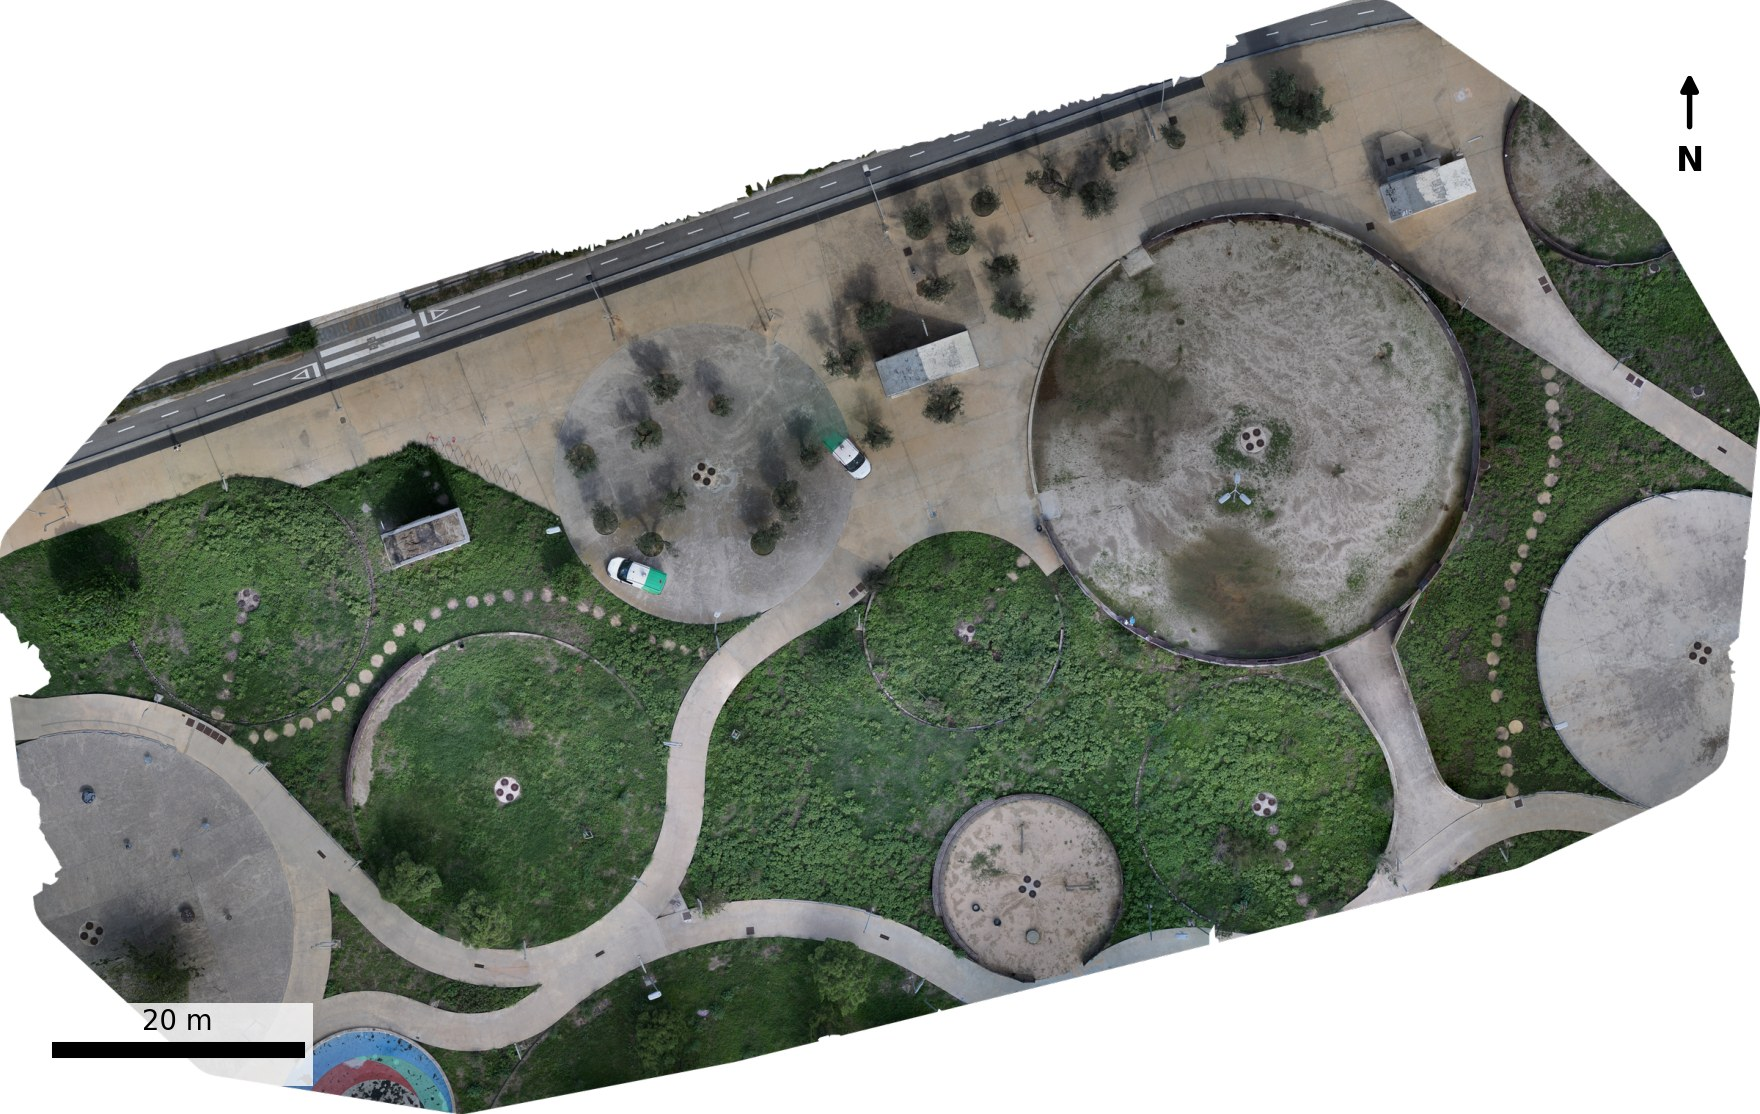
\includegraphics[width=\textwidth]{img/vol5_ortofoto.jpg}
    \caption{Orthophoto of flight test 5 (1~cm/px, EPSG:32631), processed with positions corrected for the shutter delay.}
    \label{fig:vol5-ortofoto}
\end{figure}

The orthophoto (14,084~$\times$~8,918~px at 1~cm/px) is coherent: no seams or bowl-shaped deformation, with consistent paths and roundabouts and sharp at 1:1 scale (concrete joints, individual leaves). The DSM (7,041~$\times$~4,458~px at 2~cm/px) is clean in the interior (flat buildings, trees as relief); the first and last pass and the edges show streaks because of few views, so it is advisable to crop the DSM to the polygon of interest or to extend the flight plan one \emph{footprint} beyond the area.

\begin{figure}[H]
    \centering
    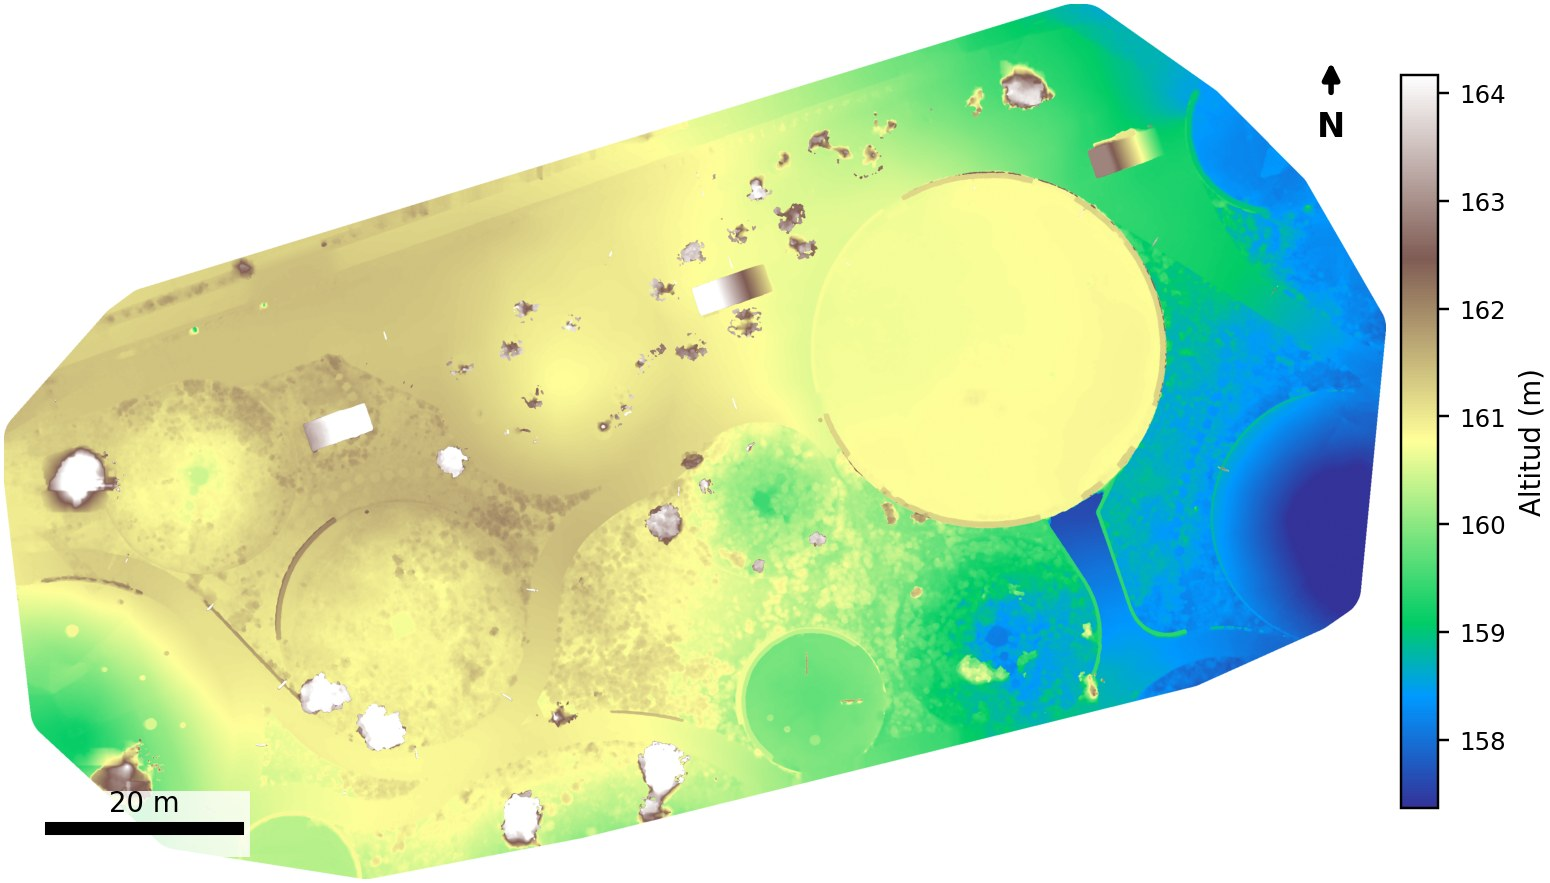
\includegraphics[width=\textwidth]{img/vol5_dsm.jpg}
    \caption{Digital surface model of flight test 5 (2~cm/px). The white gaps are treetops above the palette range.}
    \label{fig:vol5-dsm}
\end{figure}

\section{Flight test 6 -- field (13 October 2026)}
\label{sec:vol6}

\subsection{Equipment and flights}

Flight test 6 consists of two flights at $\sim$50~m (area of $\sim$180~$\times$~150~m) with the same drone and camera as 5 and with the battery parameters already calibrated. The hot-shoe \emph{feedback} (\texttt{CAM}) and the planning at 50~m were validated. They were made at dawn, with the sun between $-3^{\circ}$ and $+1^{\circ}$ above the horizon, so the photographs came out very dark.

\begin{table}[H]
    \centering
    \caption{Log of the two flights of flight test 6}
    \label{tab:vol6-logs}
    \small
    \begin{tabular}{lcc}
        \toprule
        & Flight 1 (07:46) & Flight 2 (07:57) \\
        \midrule
        mAh consumed (\texttt{CurrTot} / integral) & 2,326 / 2,306 & 2,434 / 2,426 \\
        Motors running & 5.5~min & 11.3~min (two arms) \\
        Voltage initial / minimum / final & 24.65 / 21.25 / 21.95~V & 24.73 / 21.13 / 21.95~V \\
        Current average / maximum & 25 / 56~A & 22 / 58~A \\
        Low-battery \emph{failsafe} & 268~s, 21.52~V, 1,887~mAh & 635~s, 21.48~V, 2,012~mAh \\
        Triggers \texttt{TRIG} / \texttt{CAM} / photos & 94 / 93 / 94 & 110 / 110 / 110 \\
        \bottomrule
    \end{tabular}
\end{table}

\begin{itemize}
    \item \textbf{Battery.} Both flights end by low-battery \emph{failsafe} when only 47--50~\% of the 4,000~mAh has been used: the instantaneous voltage drops below 21.6~V under load (\texttt{BATT\_FS\_VOLTSRC=0}). The mAh must be compared with what the charger returns.
    \item \textbf{Exposure.} 1/1600~s, f/5.6, ISO 1600 (ceiling of the automatic ISO): the photographs are about 6~\emph{stops} underexposed, and the scene light is 8.5--11.9~\emph{stops} below that of flight 5 (sun at 40$^{\circ}$). The maximum margin of the camera is 5.7~\emph{stops}. It is not a fault: it is a light limitation.
    \item \textbf{Feedback.} With \texttt{TRIG}, \texttt{CAM} and photographs in a 1:1 ratio (110 of 110 in flight 2), pairing is done by instant. There is one manual photo without \texttt{TRIG} and one \texttt{TRIG} without a photo.
\end{itemize}

\pendent{Repeat this flight with the sun more than 10--15$^{\circ}$ high, which is the condition that makes it usable (the current batch only serves as a test).}

\subsection{Processing of flight 2}

Flight 1 is not usable (the digital gain $\times 551$ does not recover signal: 2 matches between consecutive photos, the same as the noise). From flight 2 the 110 photographs were processed with a linear gain of $\times 2$ to $\times 97$ (median $\times 49$); \textbf{the geometry is valid, but the colours and radiometric values are not} (blue-green tint, high noise), so this batch is not suitable for colour or vegetation indices.

\begin{table}[H]
    \centering
    \caption{Processing results of flight 2 of flight test 6}
    \label{tab:vol6-resultats}
    \begin{tabular}{ll}
        \toprule
        Item & Value \\
        \midrule
        Photos reconstructed & 110 of 110 (1 component) \\
        Sparse model points / observations & 101,094 / 354,361 \\
        Reprojection error & 1.82~px \\
        Mean GSD / reconstructed area & 0.743~cm/px / 30,626~m\textsuperscript{2} \\
        Dense point cloud & 27,207,845 points \\
        Camera calibration & focal length 25.79~mm \\
        Model--GPS difference (E / N / vert.) & 0.30 / 0.32 / 0.30~m; CE90 0.57~m, LE90 0.27~m \\
        Orthophoto / DSM resolution & 3~cm/px / 5~cm/px \\
        Processing time & 29~min 42~s \\
        \bottomrule
    \end{tabular}
\end{table}

The quality is lower than in flight 5 (reprojection of 1.82~px versus 0.90~px): this is consistent with the noise of the images, which makes a larger working resolution (3~cm/px) preferable. The orthophoto (7,799~$\times$~7,071~px) shows the field, the paths, the bend of the path and a white vehicle recognisably, with a blue-green tint and noise visible and an irregular western edge. The DSM (4,679~$\times$~4,242~px) is detailed in the interior (furrows, ruts) and has streaks and an interpolation grid at the western and north-western edge.

\begin{figure}[H]
    \centering
    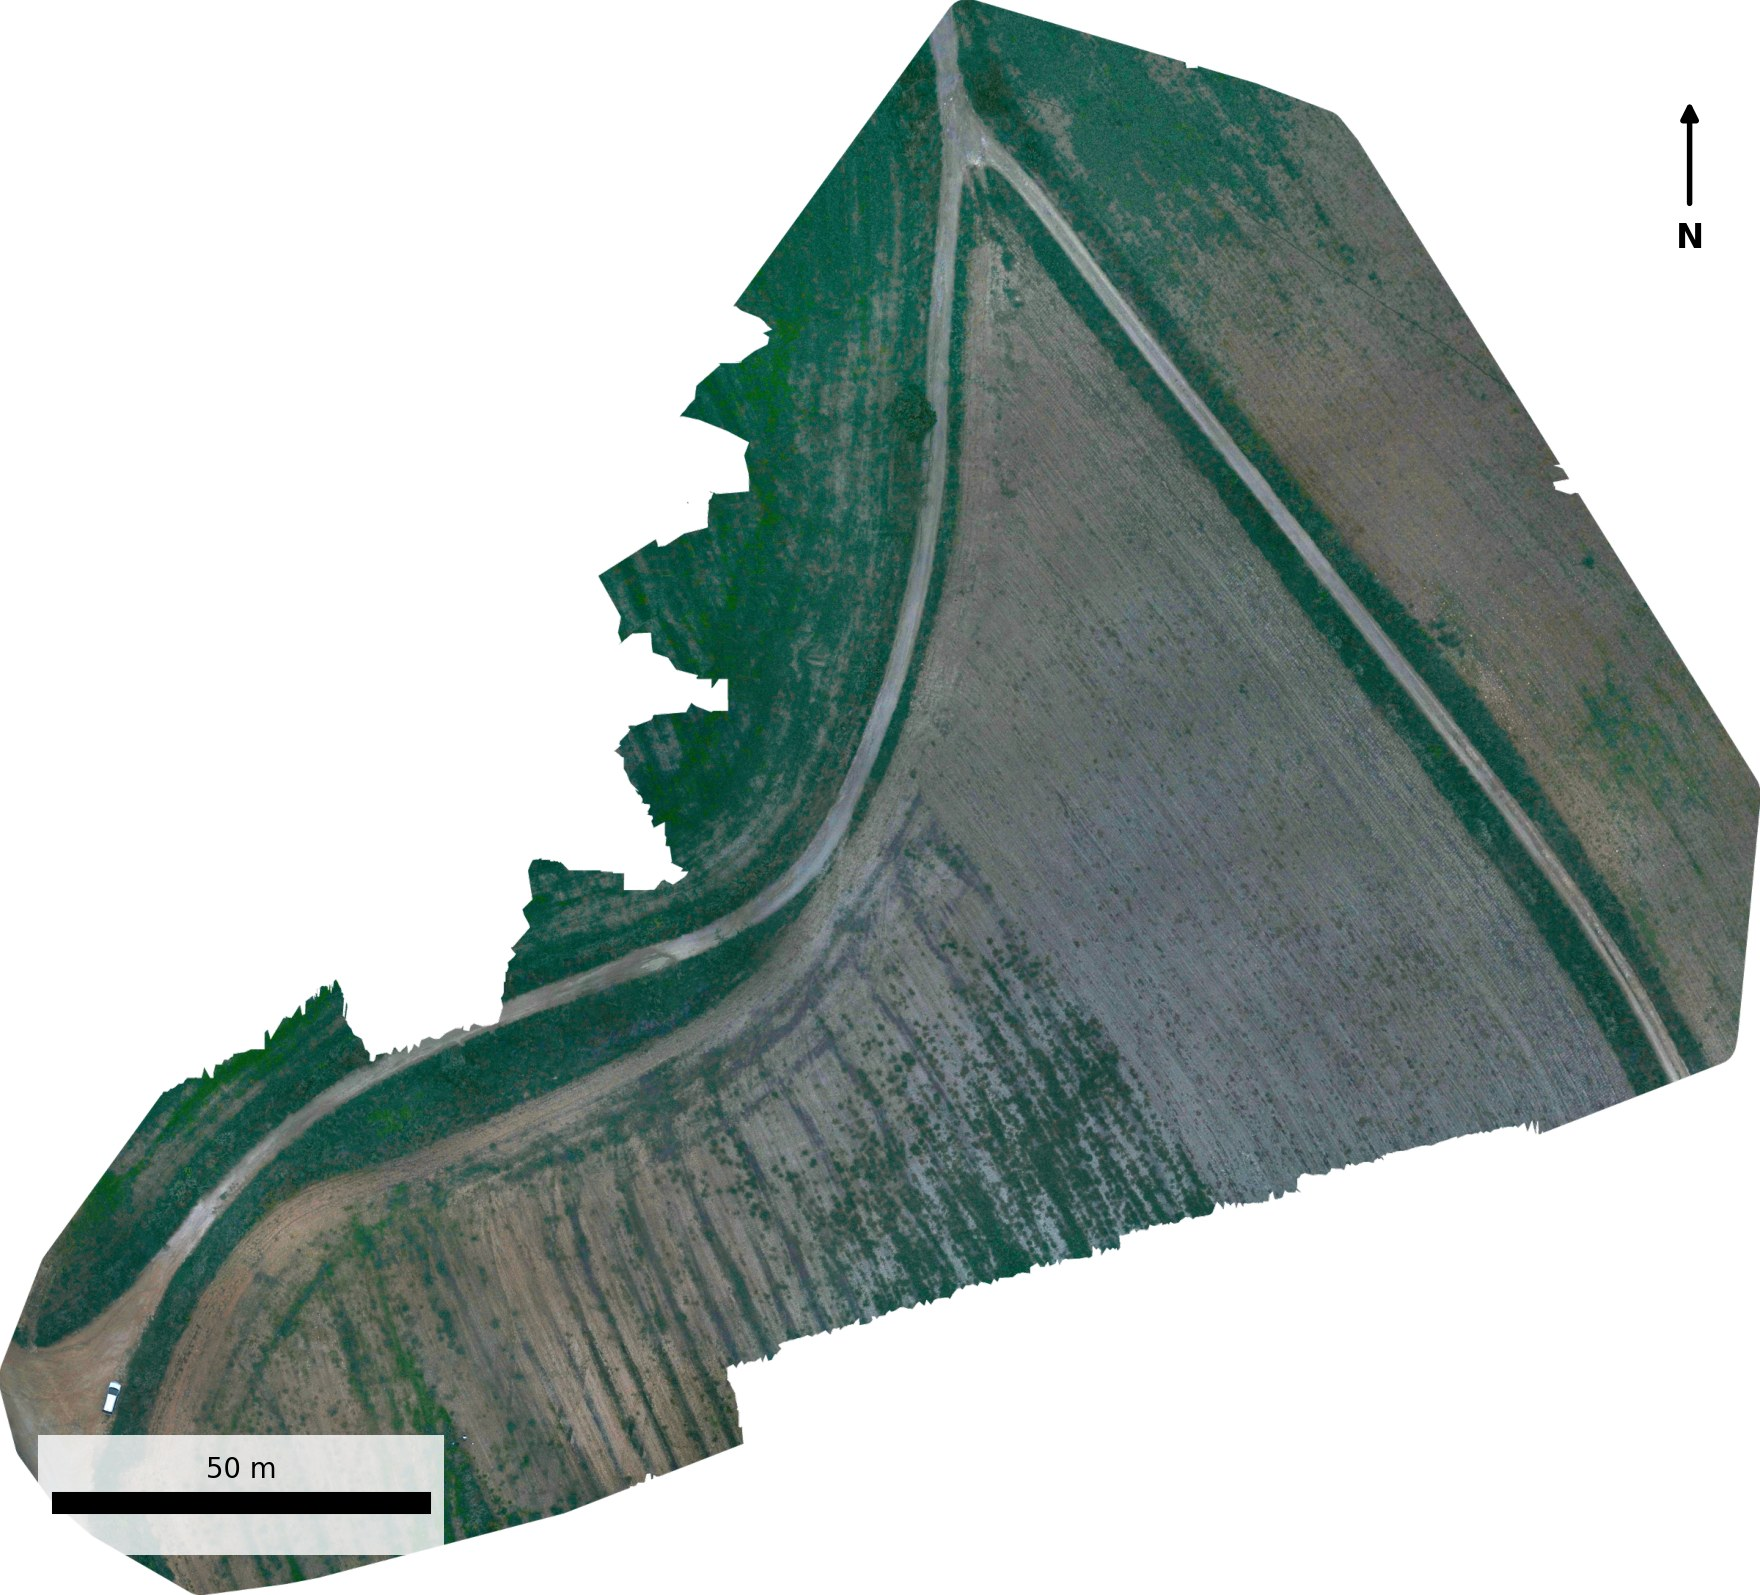
\includegraphics[width=0.85\textwidth]{img/vol6_ortofoto.jpg}
    \caption{Orthophoto of flight 2 of test 6 (3~cm/px). The images were digitally enhanced: only the geometry is valid, not the colour.}
    \label{fig:vol6-ortofoto}
\end{figure}

\begin{figure}[H]
    \centering
    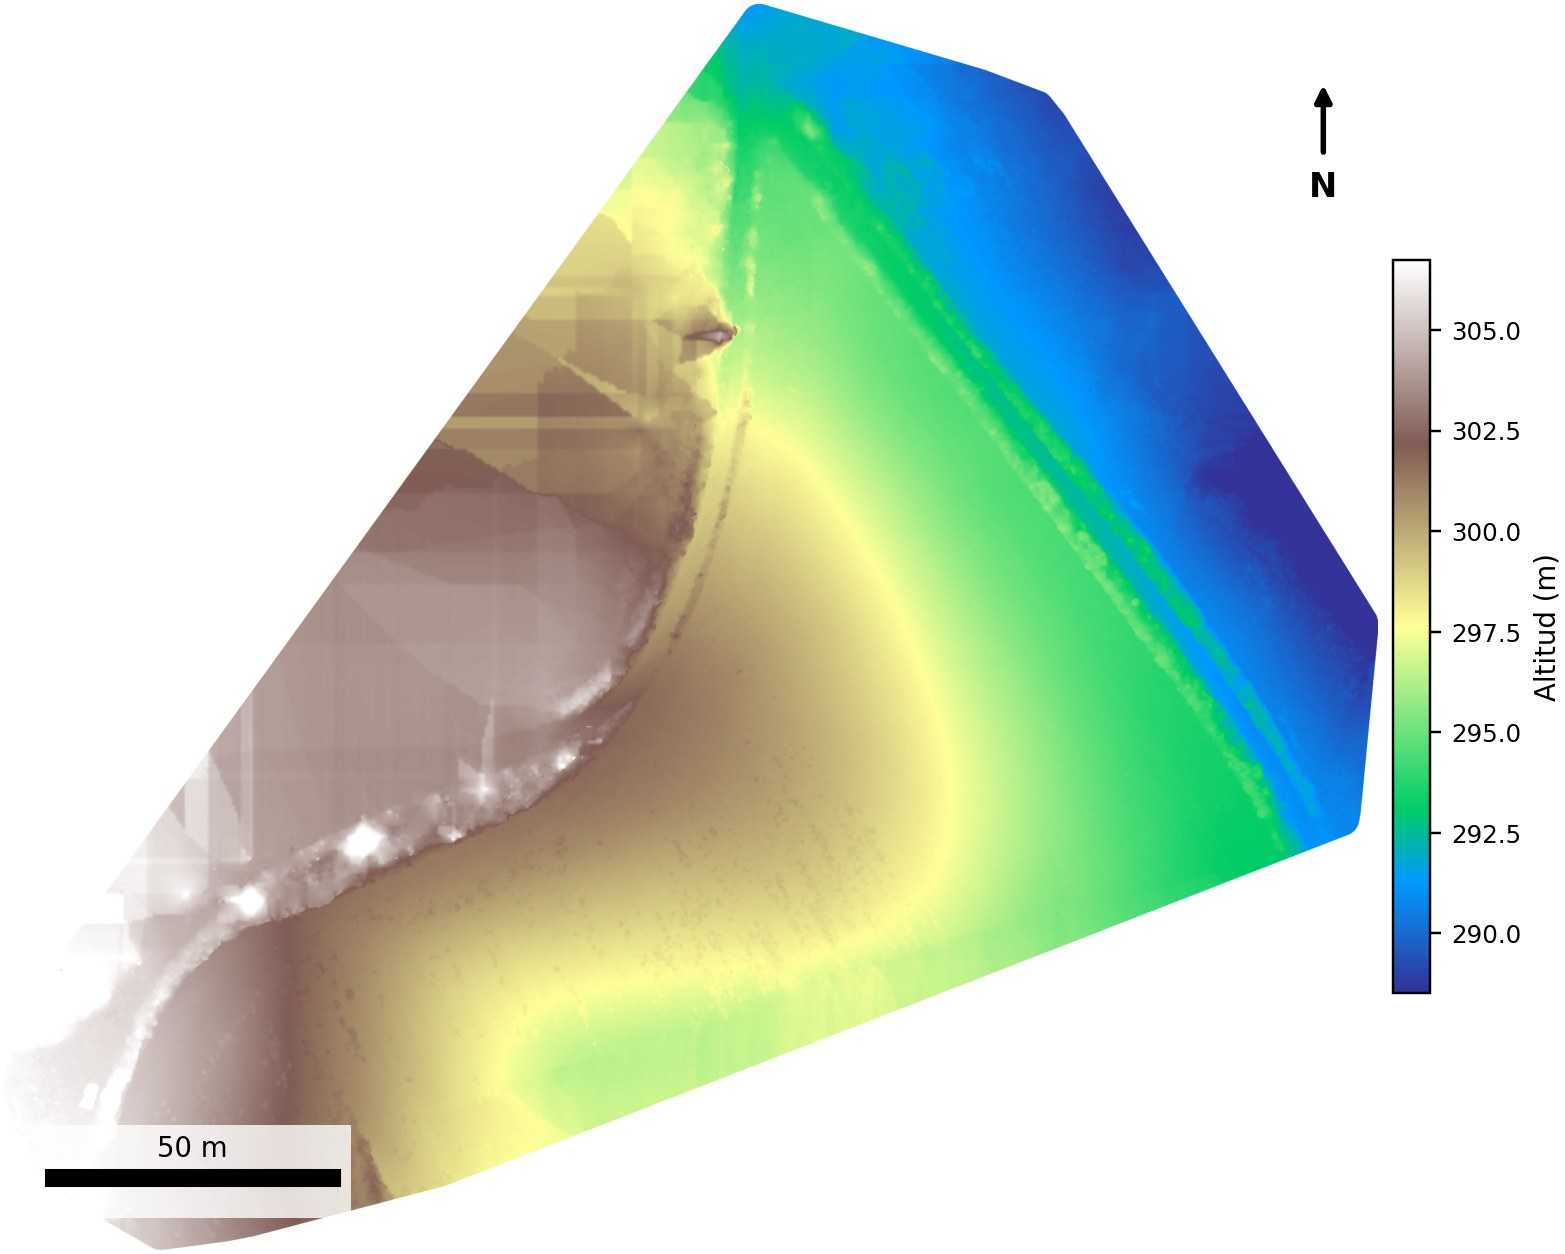
\includegraphics[width=0.85\textwidth]{img/vol6_dsm.jpg}
    \caption{Digital surface model of flight 2 of test 6 (5~cm/px).}
    \label{fig:vol6-dsm}
\end{figure}

\section{Shutter delay}
\label{sec:retard-obturador}

The trigger command of the controller and the real exposure do not coincide: between them lies the delay of the MAP2, of the camera and, possibly, of the GPS/EKF position. Since the drone moves at $\sim$5~m/s, a delay of 0.27~s equals $\sim$1.3~m of displacement, far above the centimetre-level precision sought.

\subsection{Method}

For each photo, the GPS position from the \emph{log} is compared with the camera position reconstructed by the photogrammetric model. If the delay is $\tau$, the GPS $-$ model residual is $-v\tau$: it has the opposite sign on the outbound and return passes and a global offset close to zero, which distinguishes it from a systematic georeferencing error.

\subsection{Results}

\begin{table}[H]
    \centering
    \caption{Estimates of the shutter delay}
    \label{tab:retard}
    \small
    \begin{tabular}{P{5.2cm}P{4.2cm}P{4.6cm}}
        \toprule
        Measurement & Delay & Notes \\
        \midrule
        Flight 5, \texttt{TRIG} positions & $\tau = 0.268 \pm 0.009$~s & ENE 0.277~$\pm$~0.007; WSW 0.267~$\pm$~0.014 \\
        Flight 5 with corrected positions & residual $0.004 \pm 0.007$~s & Horizontal residual median 1.38~m $\rightarrow$ 0.35--0.49~m \\
        Flight 6, \texttt{TRIG}$\rightarrow$\texttt{CAM} & median 0.34~s (0.11--0.40) & Measured directly in the \emph{log} \\
        Flight 6, \texttt{CAM} positions & residual $-0.056 \pm 0.011$~s & The \texttt{CAM} position is $\sim$56~ms ahead of the exposure \\
        Flight 6, \texttt{TRIG}$\rightarrow$exposure & $0.34 - 0.056 \approx 0.28$~s & Agrees with flight 5 by an independent route \\
        Bench, command$\rightarrow$shutter & 0.12--0.19~s & Does not explain all the delay in flight \\
        \bottomrule
    \end{tabular}
\end{table}

Two independent methods --~the photogrammetric residual of flight 5 and the combination of \texttt{TRIG}, \texttt{CAM} and residual of flight 6~-- agree on 0.27--0.28~s. It is an \emph{effective} delay: it adds up that of the shutter and, possibly, that of the GPS/EKF position, and a fixed forward offset of the antenna with respect to the camera is confounded with it (if left as an unknown, the delay comes out at 0.34~$\pm$~0.03~s and the offset at 0.32~$\pm$~0.16~m, and they cannot be separated). The bench delay does not explain the whole in-flight value; it cannot be separated without \emph{feedback}.

\subsection{Consequences for geotagging}

With \emph{feedback} (\texttt{CAM}), the position is that of the real exposure and only a residual delay of $-0.056$~s remains ($\sim$0.3~m at 5~m/s), which can be compensated. Without \emph{feedback} the position must be shifted by $v\cdot\tau$ with $\tau \approx 0.27$~s and wider per-photo precisions. This is the reason why the hot-shoe \emph{feedback} is mandatory for centimetre-level precision (\cref{sec:decisions}).

\section{Balance of the test flights}
\label{sec:balanc-vols}

\textbf{What has worked.}
\begin{itemize}
    \item The complete chain, from planning to the DSM, with RTK Fixed throughout the flight on both receivers and valid GNSS \emph{yaw}.
    \item A geometry of photogrammetric quality: reprojection of 0.90~px, 118 of 118 photos reconstructed and a GSD (0.451~cm/px) consistent with the flight height and the calibrated focal length (\cref{sec:planificacio-vol}).
    \item The hot-shoe \emph{feedback} (110 of 110 in flight 6) and the independent quantification of the shutter delay.
\end{itemize}

\textbf{Limitations.}
\begin{itemize}
    \item There are no control or check points: an absolute precision cannot be stated. The model--GPS figures are internal coherence.
    \item The absolute position depends on the RTK base, which in these flights ran a \emph{survey-in} in every session with the antenna at 122~cm (\cref{subsec:muntatge-base}). The resulting position was not recorded, and the absolute error is of the order of metres, common to the whole flight.
    \item For flight 5 the weather conditions, the in-flight mass and the battery used are not available: the \emph{log} and the photographs are the only record.
    \item Light limits the operation: flights must be made with the sun more than 10--15$^{\circ}$ high (or, with little light, 1/800~s, f/4 and ISO 3200 at the limit).
    \item Endurance is short: the low-battery \emph{failsafes} act at half consumption because of the voltage drop under load (\cref{sec:autonomia}).
    \item The DSM shows streaks at the periphery: the flight plan must be extended one \emph{footprint} beyond the area of interest.
\end{itemize}

\textbf{Next steps.} Repeat the field flight with the sun high, measure ground control and check points to establish absolute precision, re-estimate the delay with \emph{feedback} and improve endurance (\cref{sec:propulsor}). The complete list of pending tasks is in \cref{sec:pendents-proves-vol}.

\pendent{The absolute precision (horizontal and vertical) of the final product remains unmeasured: all the errors in this chapter are internal coherence.}


\backmatter
\printbibliography[title={References}]

\end{document}
